

\documentclass[12pt]{article}
\usepackage[]{geometry}
\usepackage{mathrsfs}
\usepackage{graphicx}
\usepackage[table]{xcolor}
\graphicspath{ {figures/} }
\usepackage{amsmath}
\usepackage{amssymb}
\usepackage{subfloat}
\usepackage[english]{babel}
\usepackage[T1]{fontenc}
\usepackage{amsmath,amsfonts,amssymb}
\usepackage{pdflscape}
\usepackage{natbib}
\usepackage{verbatim}
\usepackage{lipsum}
\usepackage{gensymb}
\usepackage{comment}
\usepackage{bm}
\usepackage{changepage}
\usepackage{lscape}
\usepackage{soul}
\usepackage{float}
\usepackage{rotating}
\usepackage{graphicx}
\usepackage{setspace}
\usepackage[color]{changebar}
\numberwithin{equation}{section}
\usepackage{appendix}
\usepackage{authblk}
\usepackage{hyperref}
\usepackage[most]{tcolorbox}
\usepackage{placeins}
\usepackage{caption}
\usepackage{subfig}
\usepackage{setspace}
\onehalfspacing

\setlength{\parindent}{0pt}
\setlength{\parskip}{1em}
\geometry{vmargin={1in,1in}, hmargin={.75in, .75in}}
\usepackage{fancyhdr}
\renewcommand{\headrulewidth}{0.0pt}
\renewcommand{\footrulewidth}{0.0pt}
\usepackage[labelfont={footnotesize,bf} , textfont=footnotesize]{caption}	
\captionsetup{labelformat=simple, labelsep=period}	
\setlength{\intextsep}{10pt}
\setlength{\abovecaptionskip}{2pt}
\setlength{\belowcaptionskip}{-10pt}

\renewcommand{\textfraction}{0.10}
\renewcommand{\topfraction}{0.85}
\renewcommand{\bottomfraction}{0.85}
\renewcommand{\floatpagefraction}{0.90}
\renewcommand{\baselinestretch}{1.15}

\hypersetup{colorlinks,allcolors=blue}

\title{De-anchored Expectations and Learning at the Zero Lower Bound.\\
(Preliminary and incomplete)}\vspace{10 mm} 
\author{Tolga Ozden\footnote{T.ozden@uva.nl, University of Amsterdam}}
\begin{document}

\maketitle


\bibliographystyle{apalike2}
\begin{abstract}

This paper extends on Ozden \& Wouters (2020) to assess the empirical relevance of heterogeneous expectations, learning and forward guidance at the zero lower bound in the baseline 3-equation New Keynesian model. Structural changes in monetary policy, and the heterogeneity of private sector expectations are both captured in a unified framework of endogenous regime switching. Monetary policy is subject to regime switches between an active Taylor rule during normal times, and a passive rule during the ZLB episodes, while expectations switch between an anchored Rational Expectations (RE) rule and a de-anchored learning rule. The results suggest (i) that endogenous switching models generate a reasonable fit for historical U.S. data, on par with exogenous switching models. (ii) A higher fraction of de-anchored expectations, and a higher intensity of learning can both generate deflationary spirals, leading to prolonged periods of recession. (iii) Projections with the baseline model specifications generate a probability of recovery above 50 from the COVID-induced ZLB episode \% during the next 5 years, while this probability drops significantly below 50 \% if a large proportion of expectations become de-anchored. 


\end{abstract}

\vspace{3 mm}

\noindent
\textit{JEL Classification:} E37; E65; C11; C32 . \\


\vspace{3 mm}

\noindent
\textit{Keywords:} Adaptive Learning; Heterogeneous Expectations; Endogenous-Switching Models; Bayesian Estimation of DSGE Models; Zero Lower Bound. 

\newpage


\section{Introduction}

\section{Literature Review}


categories:\\


 1) heterogeneous expectations papers \\

a new keynesian model with heterogeneous expectations, branch mcgough, 2007
-introduces heterogeneous expectations into a new keynesian model
-aggregation result for a model with nominal rigidities and heterogeneous bounded rationality, i.e. they introduce heterogeneity and bounded rationality at an individual level and obtain the IS/LM curves accordingly. 


 2) Regime switching, endogenous switching papers. Junior Maih stuff goes mainly here, same for Bianchi. Estimation work also in this category. 

 3) Forward guidance literature. Some papers will be overlapping with the heterogeneous papers. 






animal spirits, risk premia and monetary policy and the ZLB, proano and lojak, 2019
-risk-related effects of monetary policy in normal times and the ZLB periods in a stylized model with boundedly rational beliefs
-forward guidance puzzle as discussed in Del Negro 2015 and Mckay 2016: due to excess sensitivity of private consumption to interest rate changes implied by the standard euler consumption equation, as well as to the front-loading character of the new keynesian phillips cure. 
Remedies to the above problem: gabaix, introducing more discounting of the future. goy 2018, introducing heterogeneity (credibility believers and adaptive learners). Hommes and Lustenhouwer: heterogeneity and bounded rationality, they show that self-fulfilling deflationary spirals can occur depending on the central bank's credibility. 
in this work: beliefs are determined by agents' assesment of the severity of ZLB episode, rather than the evolutioary measures used in previous work ("the ZLB policy rate gap")


behavioral heterogeneity and US inflation dynamics hommes 2017
-fundamentalists and random walk believers
-aggregate and survey data
-backward-looking rule typically dominates
-use references for heterogeneity in survey expectations
-parameter estimates: phillips curve slope 0.001, intensity of choice 5.040, discount factor fixed at 0.99 when estimated on inflation data
-average fractions 0.65 vfor backward looking, autocorrelation 0.89
-parameters wehn estimated on average expectation data: 1.995 for intensity of choice, 0.002 for slope (smaller intensity suggests slower switching)
-overall: this paper presents a micro-foundation for structural breaks in the degrees of backward and forward-looking components in the phillips curve. My paper essentially adopts their approach in a New Keynesian model with more forward-looking variables.


central bank credibility and forward guidance in an estimated new keynesian model, cole, 2019
-effectiveness of forward guidance in an estimated New Keynesian model with imperfect central bank credibility. They use a game-theoretic evolutionary framework. 
-they find a relatively high estimate of Fed credibility--this is consistent with my results. They model forward guidance through surprise shocks in the monetary policy equation. However their estimate is still below the full credibility case. This result helps solve the forward guidance puzzle of Del Negro. 
Their estimated measure of credibility seems to be around 70% (100% being full credibility). The consequence of this is a dampening on the power of forward guidance. 


social learning and monetary policy at the effective lower bound
-provides a model of heterogeneous expectations that accounts for the missing disinflation and the subsequent inflation-less recovery. Coordination of expectations on below target paths may result in de-anchored expectations from central bank's target. Announcing to agents to CB's target/forecast inflation may help coordinate expectations at the right level (ergo forward guidance). But CB may lose credibility if its forecasts are not consistent with realizations, e.g. in the face of unexpected shocks. 

coordinating expectations through central bank projections, 2019, fatemeh mokhtarzadeh and peterson
experiment where subjects have to forecast output and inflation
without CB projections, subjects exhibit a wide range of heuristics involving backward-looking components
CB projections nudge expectations in the direction of the REE 
CB credibility is significantly diminished when the CB makes larger forecast errors
findings suggest that CB's should ignore agents' irrationalities when constructing projections, and communicate easy to process information

busetti paper
benchmark case: VAR(1) learning with fixed mean, AR(1) learning that also includes intercept. Standard heuristic switching between the two. 

counterfactuals---sequence of deflationary shocks, what happens under REE and what happens under switching





check references
central bank credibility cole 2019
hommes behavioral heterogeneity 2017
busetti



\section{Model Setup}

Standard NK Model with indexation: 
\begin{equation}
\begin{cases}
	y_t = (1-\iota_y) E_{t-1} y_{t+1} +\iota_y y_{t-1} - \frac{1}{\tau}(r_t - E_{t-1} \pi_{t+1}) + u_{y,t} \\

\pi_t = \beta  ((1-\iota_p) E_{t-1} \pi_{t+1} + \iota_p \pi_{t-1}) + \gamma y_t  + u_{\pi,t}\\
r_t = \rho_r r_{t-1} + (1-\rho_r) (\phi_{\pi} \pi_t + \phi_y y_t) + \phi_{\delta y} (y_t - y_{t-1}) +u_{r,t}
\end{cases}
\end{equation}

AR(1) shocks: 
\begin{equation}
\begin{cases}
u_{y,t} = \rho_y u_{y,t-1} + \varepsilon_{y,t} \\
u_{\pi,t} = \rho_{\pi} u_{\pi,t-1} + \varepsilon_{\pi,t} \\
u_{r,t} = \rho_r u_{r,t-1} + \varepsilon_{r,t} \\

\end{cases}
\end{equation}

1-step ahead expectations (nowcasts) given as a VAR(1) system: 




\section{Estimations}

\subsection{Parameter Estimations, Priors and Posteriors}

\begin{table}[hbt!]
\begin{tabular}{l|lll|ll}
Param. & Dist. & Prior Mean & Prior St. Dev. & Lower B. & Upper B. \\
\hline
\hline
$\bar{\pi}$ & Uniform & 0.5 & 0.29 & 0 & $\infty$ \\
$\bar{r}$ & Uniform & 0.5 & 0.29 & 0 & $\infty$ \\
$\kappa$ & Beta & 0.05 & 0.025 & 0 & 1 \\
$\tau$ & Gamma & 2 & 0.5 & 0 & $\infty$ \\
$\phi_{\pi}$ & Gamma & 1.5 & 0.25 & 1 & $\infty$ \\
$\phi_y$ & Gamma & 0.25 & 0.1 & 0 & $\infty$ \\
$\phi_{\Delta y}$ & Gamma & 0.25 & 0.1 & 0 & $\infty$ \\
$\rho_y$ & Beta & 0.5 & 0.2 & 0 & 1 \\
$\rho_{\pi}$ & Beta & 0.5 & 0.2 & 0 & 1 \\
$\rho_r$ & Beta & 0.5 & 0.2 & 0 & 1 \\
$\eta_y$ & Inv. Gamma & 0.1 & 2 & 0 & $\infty$ \\
$\eta_pi$ & Inv. Gamma & 0.1 & 2 & 0 & $\infty$ \\
$\eta_r$ & Inv. Gamma & 0.1 & 2 & 0 & $\infty$ \\
$\iota_y$ & Beta & 0.25 & 0.1 & 0 & 1 \\
$\iota_{\pi}$ & Beta & 0.25 & 0.1 & 0 & 1 \\
$\bar{r_2}$ & Normal & 0.1 & 0.25 & 0 & $\infty$ \\
$\eta_{r_2}$ & Uniform & 0.5 & 0.29 & 0 & $\infty$ \\
$\frac{\Phi_1}{1000}$ & Gamma & 0.2 & 0.1 & 0 & $\infty$ \\
$\frac{\Phi_2}{1000}$ & Gamma & 0.2 & 0.1 & 0 & $\infty$ \\
$\gamma$ & Gamma & 0.035 & 0.015 & 0 & 1 \\
$\omega$ & Beta & 0.5 & 0.2 & 0 & 1 \\
$\chi$ & Gamma & 5 & 2 & 0 & $\infty$ \\
$1-p_{11}$ & Uniform & 0.5 & 0.29 & 0 & 1 \\
$1-p_{22}$ & Uniform & 0.5 & 0.29 & 0 & 1
\end{tabular}
\end{table}



\begin{sidewaystable}[hbt!]

\resizebox{\textwidth}{!}{\begin{tabular}{l|lll|lll||lll|lll}
% & Rational Models &  &  &  &  &  & Learning Models  &  &  &  \\
 & REE &  &  & RISE &  &  & VAR(1) &  &  & VAR(1) &  \\
 & 1 regime &  &  & 2 regime &  &  & 2 regime &  &  & 4 regime  &  \\
Param. &  Mean & 90 \% HPD & Interval &  Mean & 90 \% HPD & Interval &  Mean & 90 \% HPD & Interval & Mean & 90 \% HPD & Interval \\
$\bar{\pi}$ & 0.624 & 0.473 & 0.768 & 0.704 & 0.519 & 0.882 & 0.43 & 0.26 & 0.601 & 0.448 & 0.364 & 0.537 \\
$\bar{r}$ & 0.633 & 0.198 & 1.023 & 0.793 & 0.252 & 1.312 & 0.182 & 0.01 & 0.389 & 0.27 & 0.056 & 0.489 \\
$\kappa$ & 0.003 & 0.001 & 0.005 & 0.002 & 0.001 & 0.004 & 0.01 & 0.002 & 0.019 & 0.003 & 0.001 & 0.006 \\
$\tau$ & 2.443 & 1.711 & 3.248 & 3.525 & 2.479 & 4.606 & 1.435 & 1.127 & 1.789 & 1.532 & 1.163 & 1.934 \\
$\phi_{\pi}$ & 1.771 & 1.311 & 2.25 & 1.721 & 1.276 & 2.221 & 1.648 & 1.149 & 2.156 & 1.959 & 1.512 & 2.413 \\
$\phi_y$ & 0.146 & 0.058 & 0.245 & 0.161 & 0.068 & 0.271 & 0.203 & 0.084 & 0.326 & 0.116 & 0.055 & 0.179 \\
$\phi_{\Delta y}$ & 0.221 & 0.167 & 0.28 & 0.194 & 0.147 & 0.241 & 0.211 & 0.151 & 0.273 & 0.219 & 0.168 & 0.274 \\
$\rho_y$ & 0.595 & 0.371 & 0.781 & 0.942 & 0.913 & 0.97 & 0.953 & 0.921 & 0.983 & 0.967 & 0.95 & 0.984 \\
$\rho_{\pi}$ & 0.965 & 0.94 & 0.989 & 0.625 & 0.44 & 0.795 & 0.582 & 0.298 & 0.829 & 0.553 & 0.354 & 0.73 \\
$\rho_r$ & 0.922 & 0.893 & 0.952 & 0.919 & 0.884 & 0.951 & 0.936 & 0.903 & 0.967 & 0.89 & 0.854 & 0.927 \\
$\eta_y$ & 0.052 & 0.035 & 0.07 & 0.033 & 0.018 & 0.048 & 0.095 & 0.063 & 0.131 & 0.089 & 0.06 & 0.119 \\
$\eta_pi$ & 0.049 & 0.033 & 0.068 & 0.045 & 0.029 & 0.06 & 0.062 & 0.042 & 0.087 & 0.058 & 0.043 & 0.073 \\
$\eta_r$ & 0.136 & 0.112 & 0.161 & 0.13 & 0.111 & 0.15 & 0.134 & 0.111 & 0.16 & 0.138 & 0.115 & 0.162 \\
$\iota_y$ & 0.274 & 0.199 & 0.348 & 0.243 & 0.169 & 0.317 & 0.113 & 0.059 & 0.174 & 0.322 & 0.244 & 0.401 \\
$\iota_{\pi}$ & 0.293 & 0.173 & 0.418 & 0.273 & 0.165 & 0.391 & 0.213 & 0.059 & 0.399 & 0.344 & 0.242 & 0.441 \\
$\bar{r_2}$ & - & - & - & 0.01 & 0.007 & 0.013 & 0.032 & 0.028 & 0.036 & 0.032 & 0.029 & 0.036 \\
$\eta_{r_2}$ &- & -  & - & 0.032 & 0.029 & 0.036 & 0.01 & 0.007 & 0.013 & 0.01 & 0.007 & 0.013 \\
$\frac{\Phi_1}{1000}$ & - & - & - & - & - & - & 0.177 & 0.067 & 0.312 & 0.167 & 0.065 & 0.309 \\
$\frac{\Phi_2}{1000}$ & - & - & - & - & - & - & 0.147 & 0.045 & 0.271 & 0.134 & 0.047 & 0.246 \\
$\gamma$ & -  & - & - & - & - & - & 0.007 & 0.003 & 0.01 & 0.009 & 0.003 & 0.016 \\
$\omega$ & - & - & - & - & - & - & - & - & - & 0.721 & 0.386 & 0.993 \\
$\chi$ & - & - & - & - & - & - & - & - & - & 2.093 & 0.551 & 3.896 \\
$1-p_{22}$ & - & - & - & 0.207 & 0.127 & 0.304 & - & - & - & - &-  & - \\
$1-p_{11}$ & - & - & - & 0.037 & 0.008 & 0.069 & - & - & - & - & - & - \\
\hline
\hline
 Laplace &  & 46.71 &  &   & 61.09 &  &   & 56.27 &  &  & 53.86 &  \\
 MHM & & 46.9 &  &   & 62.82 &  &  & 63.52 &  &   & 56.81 &  \\
Mode &  & 89.07 &  &   & 122.09 &  &   & 126.01 &  &   & 122.99 & 
\end{tabular}}
\end{sidewaystable}



\begin{sidewaystable}[hbt!]
\resizebox{\textwidth}{!}{\begin{tabular}{l|lll|lll||lll|lll}
% & Rational Models &  &  &  &  &  & Learning Models  &  &  &  \\
 & REE &  &  & RISE &  &  & AR(1)&  &  & AR(1)  &  \\
 & 1 regime &  &  & 2 regime &  &  & 2 regime &  &  & 4 regime  &  \\
Param. & Mean & 90 \% HPD & Interval &  Mean & 90 \% HPD Interval  & &  Mean & 90 \% HPD & Interval &  Mean & 90 \% HPD & Interval \\
$\bar{\pi}$ & 0.624 & 0.473 & 0.768 & 0.704 & 0.519 & 0.882 & 0.599 & 0.329 & 0.857 & 0.516 & 0.428 & 0.609 \\
$\bar{r}$ & 0.633 & 0.198 & 1.023 & 0.793 & 0.252 & 1.312 & 0.588 & 0.001 & 1.077 & 0.28 & 0.005 & 0.543 \\
$\kappa$ & 0.003 & 0.001 & 0.005 & 0.002 & 0.001 & 0.004 & 0.009 & 0.003 & 0.015 & 0.001 & 0.0002 & 0.003 \\
$\tau$ & 2.443 & 1.711 & 3.248 & 3.525 & 2.479 & 4.606 & 2.924 & 1.747 & 4.056 & 2.147 & 1.809 & 2.495 \\
$\phi_{\pi}$ & 1.771 & 1.311 & 2.25 & 1.721 & 1.276 & 2.221 & 1.572 & 1.106 & 2.032 & 1.732 & 1.296 & 2.2 \\
$\phi_y$ & 0.146 & 0.058 & 0.245 & 0.161 & 0.068 & 0.271 & 0.164 & 0.056 & 0.275 & 0.209 & 0.117 & 0.308 \\
$\phi_{\Delta y}$ & 0.221 & 0.167 & 0.28 & 0.194 & 0.147 & 0.241 & 0.14 & 0.103 & 0.177 & 0.2 & 0.162 & 0.237 \\
$\rho_y$ & 0.595  & 0.371  & 0.781 & 0.942 & 0.913 & 0.97 & 0.708 & 0.507 & 0.926 & 0.946 & 0.918 & 0.973 \\
$\rho_{\pi}$ & 0.965 &0.94  &0.989   & 0.625 & 0.44 & 0.795 & 0.419 & 0.218 & 0.641 & 0.487 & 0.277 & 0.717 \\
$\rho_r$ & 0.922 & 0.893 & 0.952 & 0.919 & 0.884 & 0.951 & 0.944 & 0.913 & 0.973 & 0.916 & 0.884 & 0.949 \\
$\eta_y$ & 0.052 & 0.035 & 0.07 & 0.033 & 0.018 & 0.048 & 0.252 & 0.141 & 0.365 & 0.107 & 0.079 & 0.138 \\
$\eta_pi$ & 0.049 & 0.033 & 0.068 & 0.045 & 0.029 & 0.06 & 0.061 & 0.041 & 0.082 & 0.06 & 0.04 & 0.077 \\
$\eta_r$ & 0.136 & 0.112 & 0.161 & 0.13 & 0.111 & 0.15 & 0.119 & 0.104 & 0.136 & 0.134 & 0.113 & 0.154 \\
$\iota_y$ & 0.274 & 0.199 & 0.348 & 0.243 & 0.169 & 0.317 & 0.41 & 0.205 & 0.599 & 0.41 & 0.358 & 0.463 \\
$\iota_{\pi}$ & 0.293 & 0.173 & 0.418 & 0.273 & 0.165 & 0.391 & 0.266 & 0.119 & 0.41 & 0.396 & 0.3 & 0.483 \\
$\bar{r_2}$ & - & - & - & 0.01 & 0.007 & 0.013 & 0.032 & 0.029 & 0.036 & 0.032 & 0.029 & 0.036 \\
$\eta_{r_2}$ & - & - & - & 0.032 & 0.029 & 0.036 & 0.01 & 0.007 & 0.013 & 0.01 & 0.007 & 0.013 \\
$\frac{\Phi_1}{1000}$ & - & - & - & - & - & - & 0.263 & 0.09 & 0.458 & 0.176 & 0.074 & 0.316 \\
$\frac{\Phi_2}{1000}$ & - & - & - & - & - & - & 0.093 & 0.02 & 0.237 & 0.122 & 0.032 & 0.255 \\
$\gamma$ & - & - & - & - & - & - & 0.013 & 0.004 & 0.023 & 0.025 & 0.008 & 0.042 \\
$\omega$ & - & - & - & - & - & - & - & - & - & 0.633 & 0.285 & 0.998 \\
$\chi$ & - & - & - & - & - & - & - & - & -  & 1.476 & 0.378 & 2.821 \\
$1-p_{22}$ & - & - & - & 0.207 & 0.127 & 0.304 & - & - & - & - & - & - \\
$1-p_{11}$ & - & - & - & 0.037 & 0.008 & 0.069 & - & - & - & - & - & -	 \\
\hline
\hline
Laplace &  & 46.71 &  &   & 61.09 &  &  &   & 51.028 &  &   & 50.74 \\
MHM &  & 46.9 &  &   & 62.82 &  &  &   & 53.15 &  &   & 50.15 \\
Mode &  & 89.07 &  &   & 122.09 &  &  &   & 107.42 &  &  & 110.53
\end{tabular}}
\end{sidewaystable}




\FloatBarrier

\subsection{Figures and Tables for 4-regime VAR(1) Model}







\begin{sidewaysfigure}[hbt!]
\centerline{
\subfloat[$\alpha_y$]{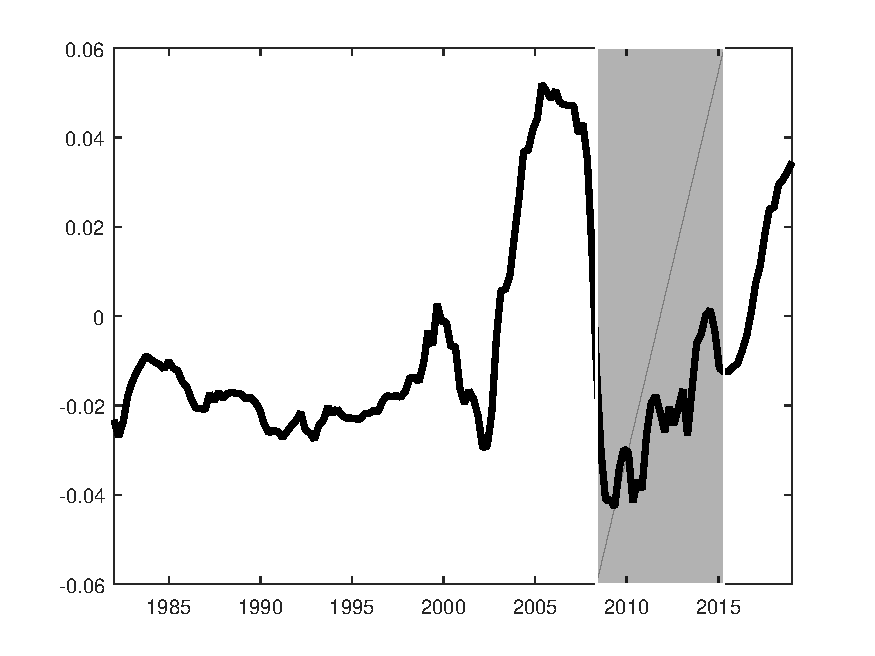
\includegraphics[scale=0.4]{figures/var1_4regime_alpha1.pdf}}
\subfloat[$\beta_{y,\pi}$]{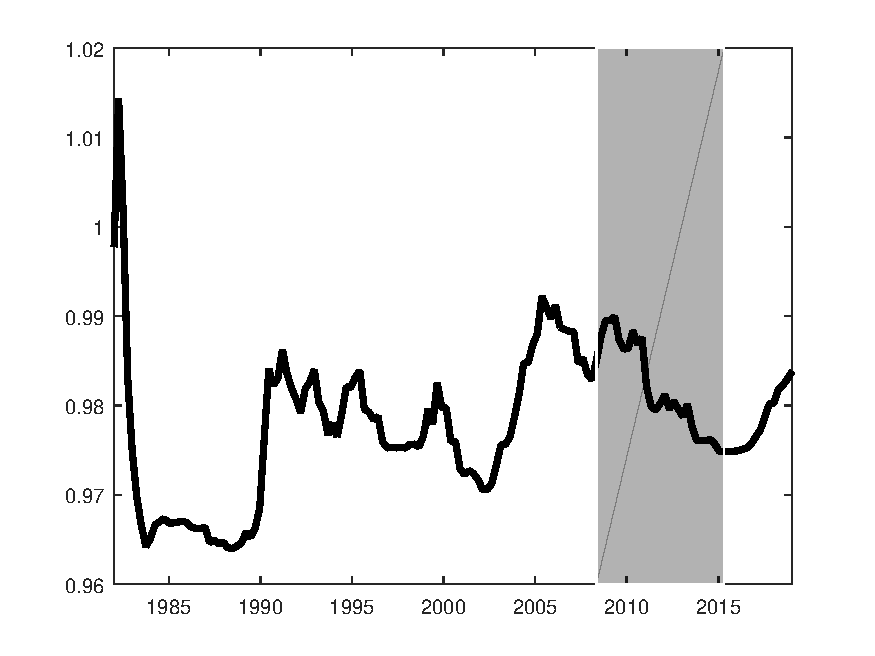
\includegraphics[scale=0.4]{figures/var1_4regime_beta11.pdf}}
\subfloat[$\beta_{y,y}$]{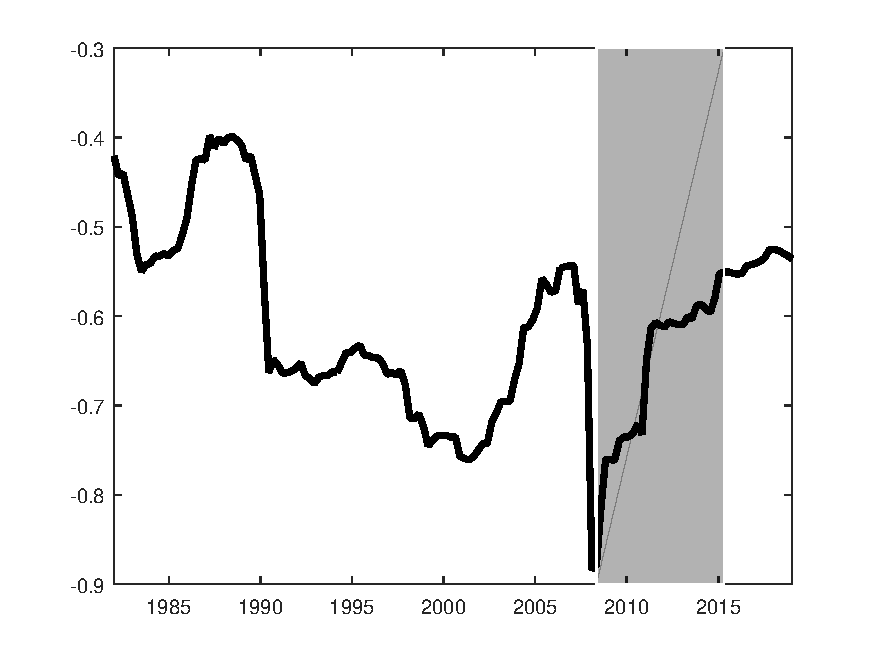
\includegraphics[scale=0.4]{figures/var1_4regime_beta12.pdf}}
\subfloat[$\beta_{y,r}$]{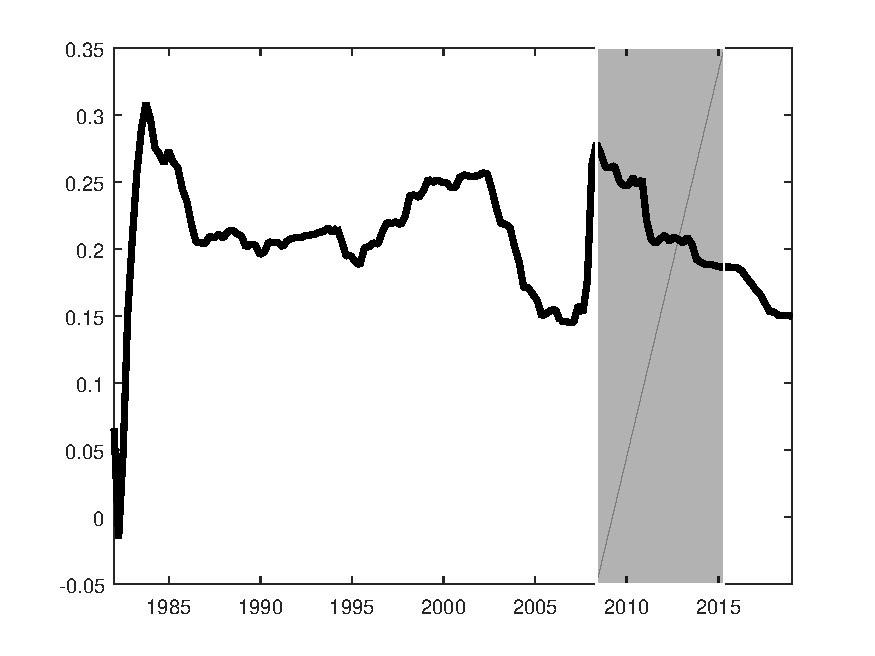
\includegraphics[scale=0.4]{figures/var1_4regime_beta13.pdf}}
} 

\centerline{
\subfloat[$\alpha_{\pi}$]{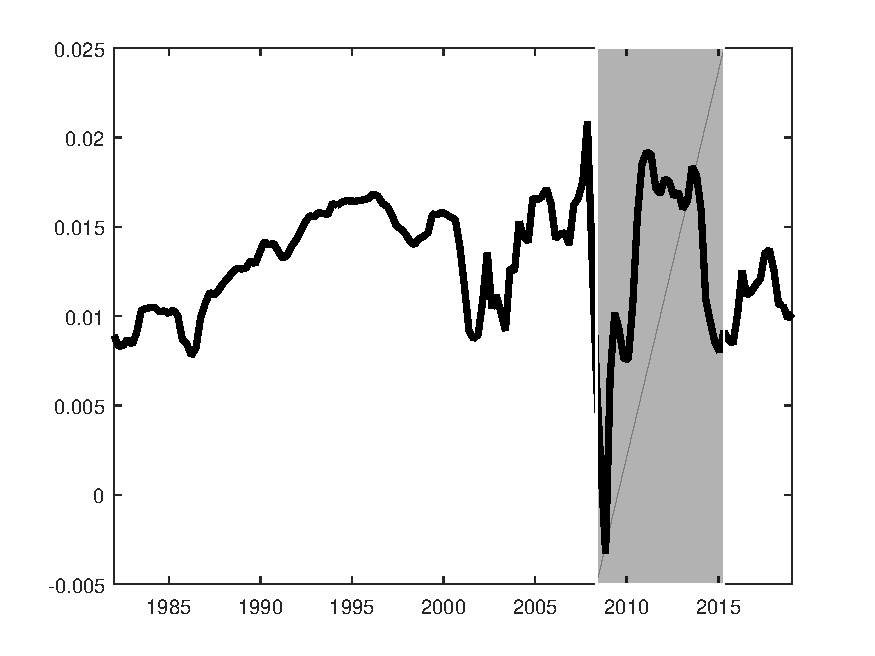
\includegraphics[scale=0.4]{figures/var1_4regime_alpha2.pdf}}
\subfloat[$\beta_{\pi,\pi}$]{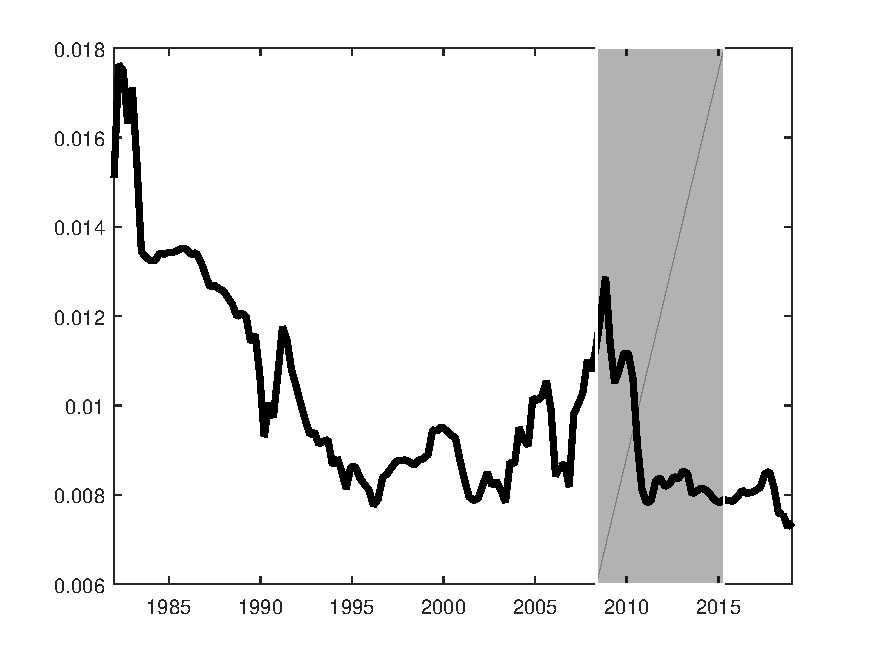
\includegraphics[scale=0.4]{figures/var1_4regime_beta21.pdf}}
\subfloat[$\beta_{\pi,y}$]{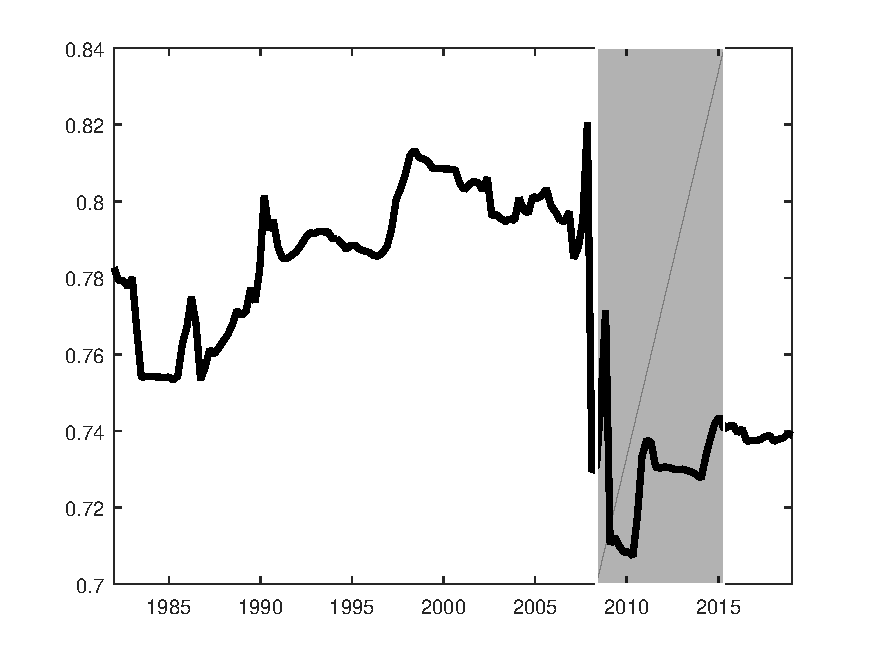
\includegraphics[scale=0.4]{figures/var1_4regime_beta22.pdf}}
\subfloat[$\beta_{\pi,r}$]{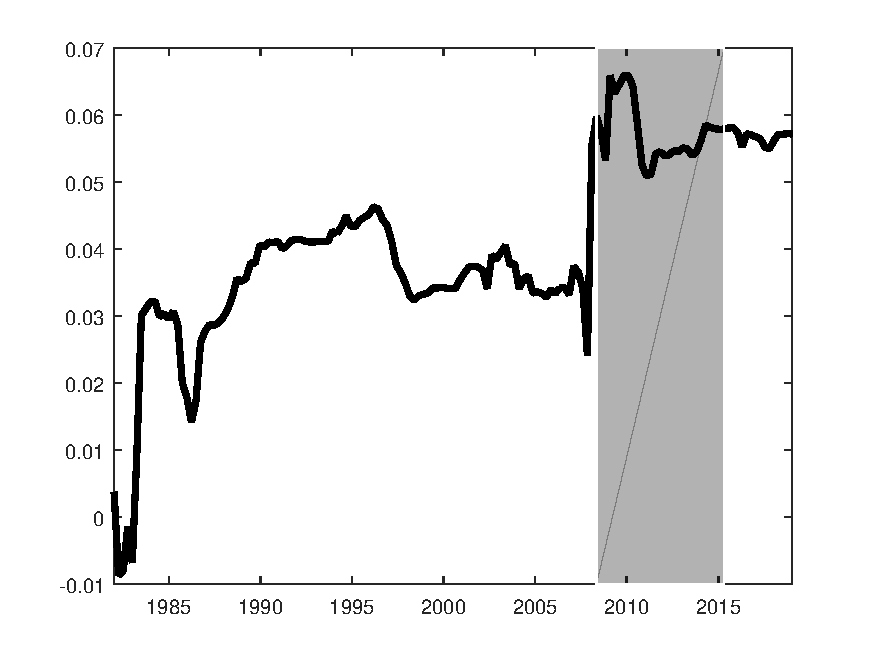
\includegraphics[scale=0.4]{figures/var1_4regime_beta23.pdf}}
} 
\caption{4-regime model, perceived $\alpha$ and $\beta$ coefficients.}
\end{sidewaysfigure}



\begin{figure}[hbt!]
\centerline{
\subfloat[$\alpha_y$]{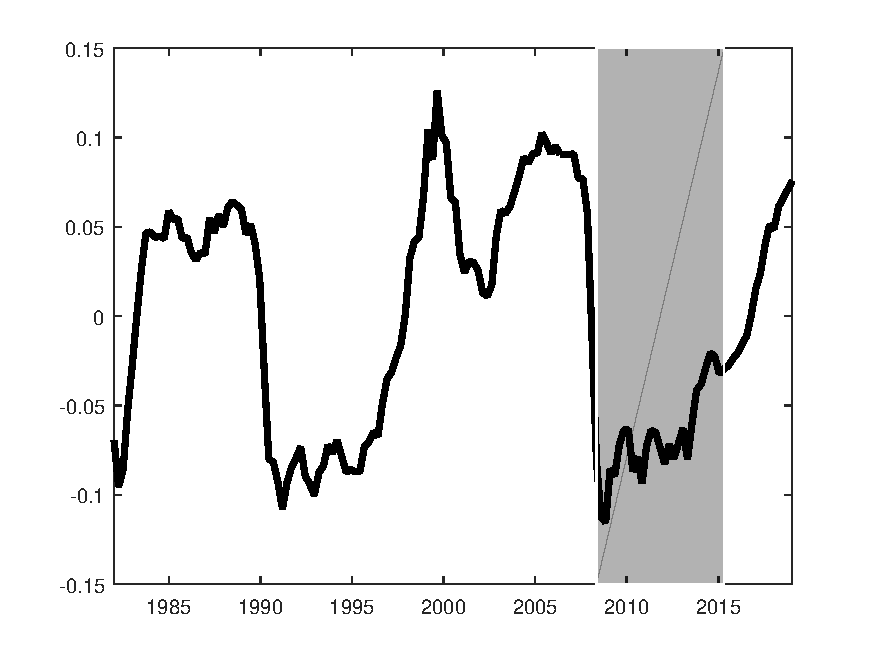
\includegraphics[scale=0.4]{figures/ar1_4regime_alpha1.pdf}}
\subfloat[$\beta_{y,y}$]{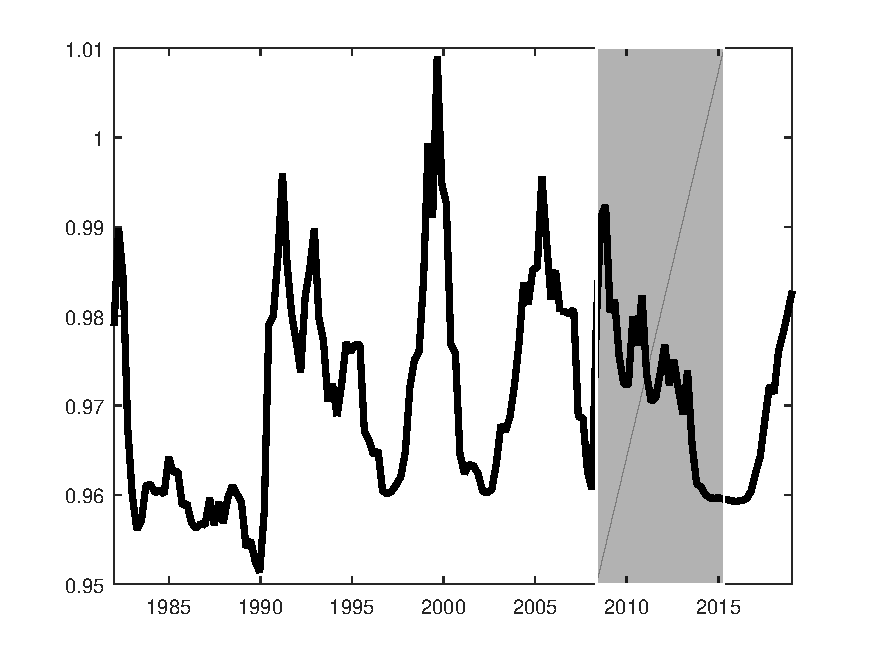
\includegraphics[scale=0.4]{figures/ar1_4regime_beta11.pdf}}
} 

\centerline{
\subfloat[$\alpha_{\pi}$]{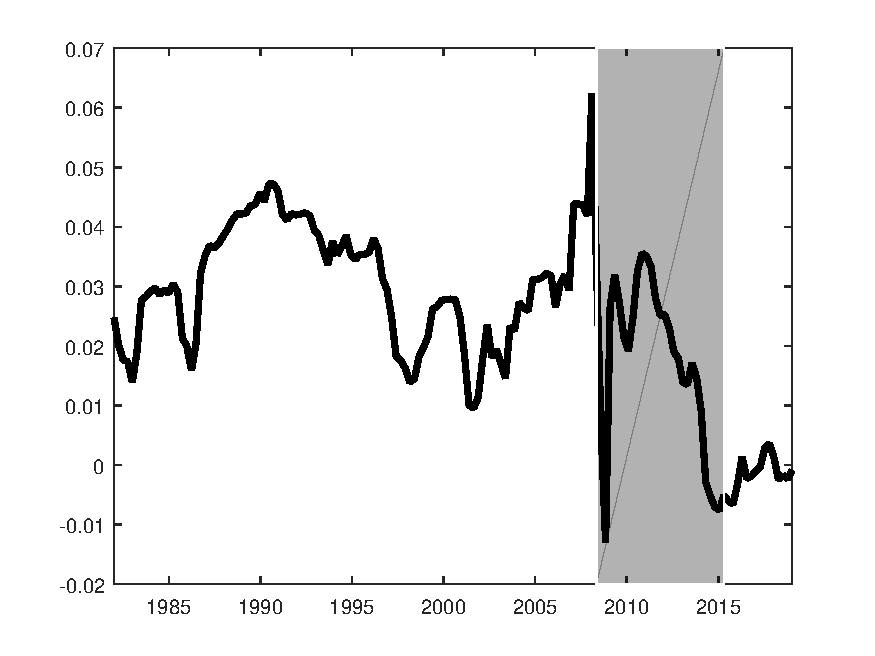
\includegraphics[scale=0.4]{figures/ar1_4regime_alpha2.pdf}}
\subfloat[$\beta_{\pi,y}$]{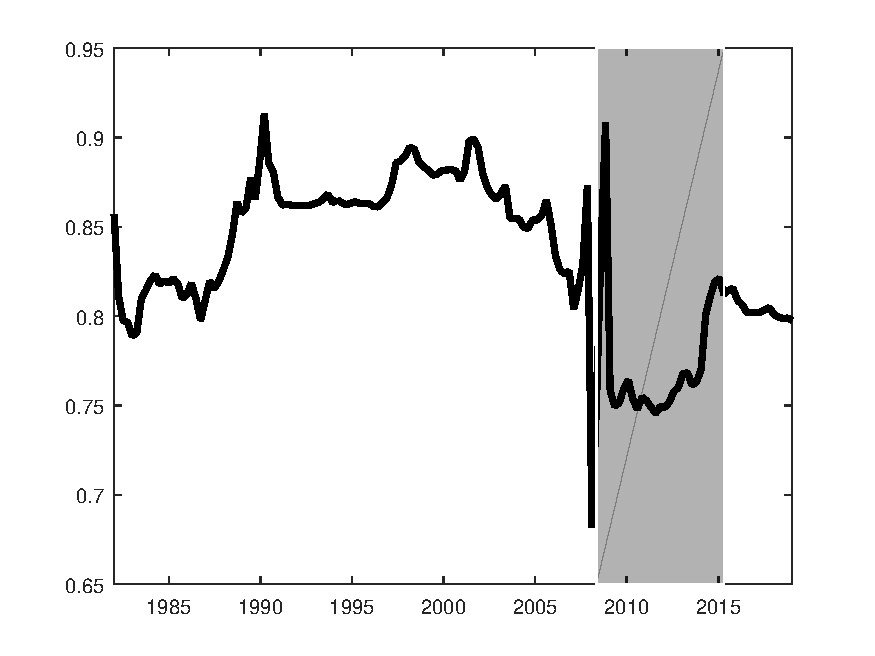
\includegraphics[scale=0.4]{figures/ar1_4regime_beta22.pdf}}
} 
\caption{4-regime model AR(1) model, perceived $\alpha$ and $\beta$ coefficients.}
\end{figure}


\begin{figure}[hbt!]
\centerline{
\subfloat[VAR(1)]{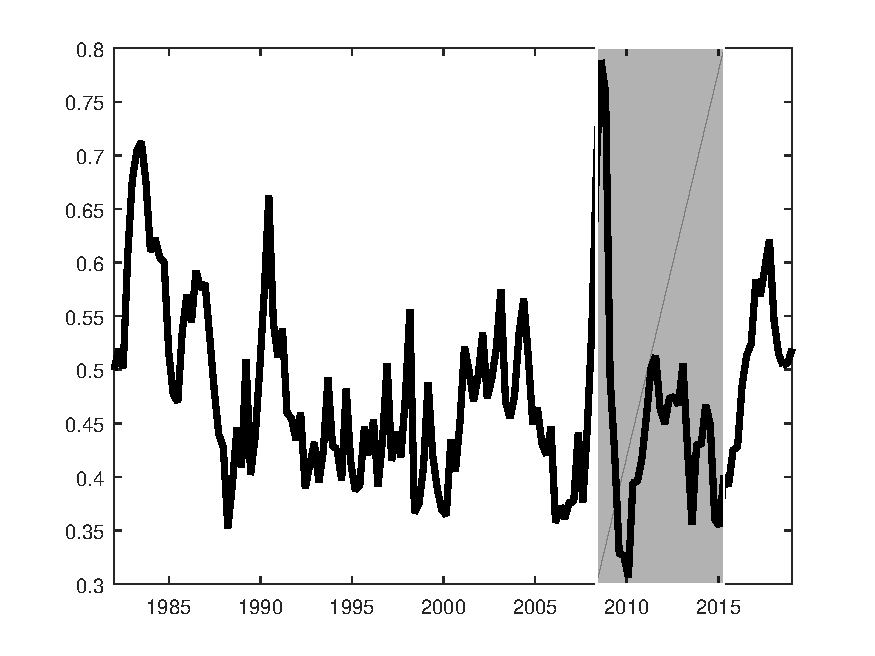
\includegraphics[scale=0.6]{figures/var1_4regime_fractions_ree.pdf}}
\subfloat[AR(1)]{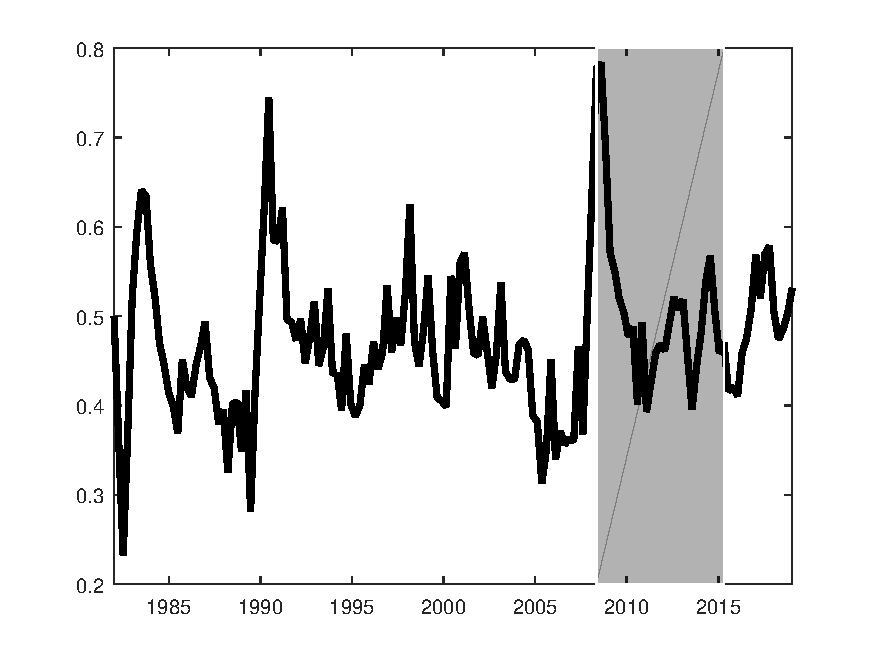
\includegraphics[scale=0.6]{figures/ar1_4regime_fractions_ree.pdf}}
}
\caption{Fraction of agents using the Determinate RE solution.}
\end{figure}


\begin{figure}[hbt!]
\centerline{\subfloat[Regime 1]{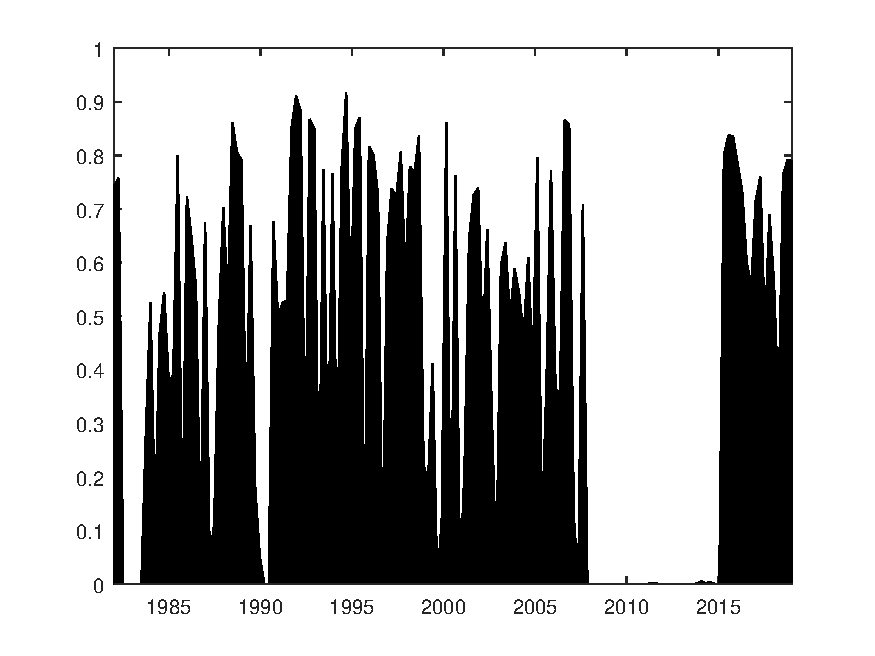
\includegraphics[scale=0.4]{figures/var1_4regime_regime1.pdf}}
\subfloat[Regime 2]{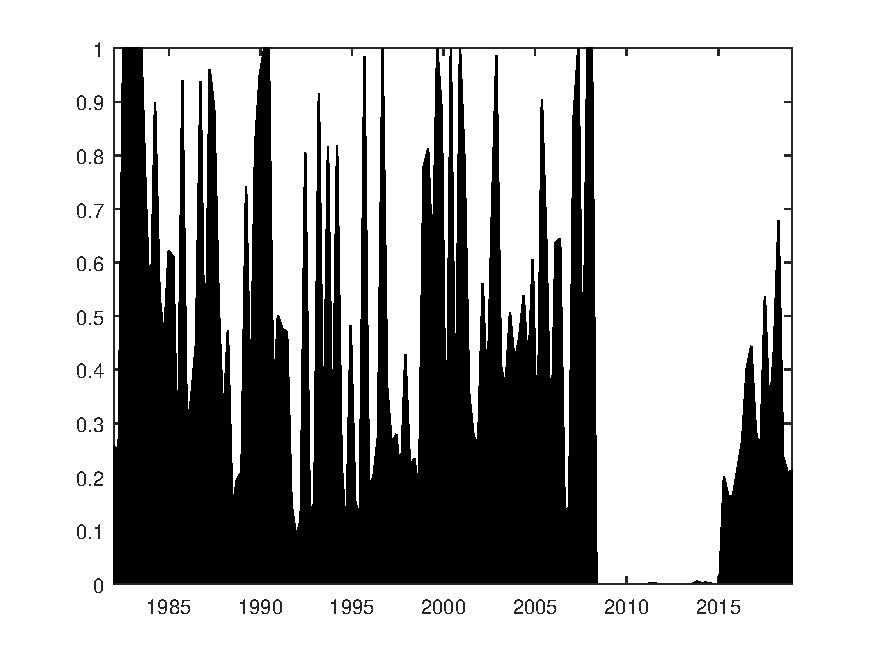
\includegraphics[scale=0.4]{figures/var1_4regime_regime2.pdf}}}

\centerline{\subfloat[Regime 3]{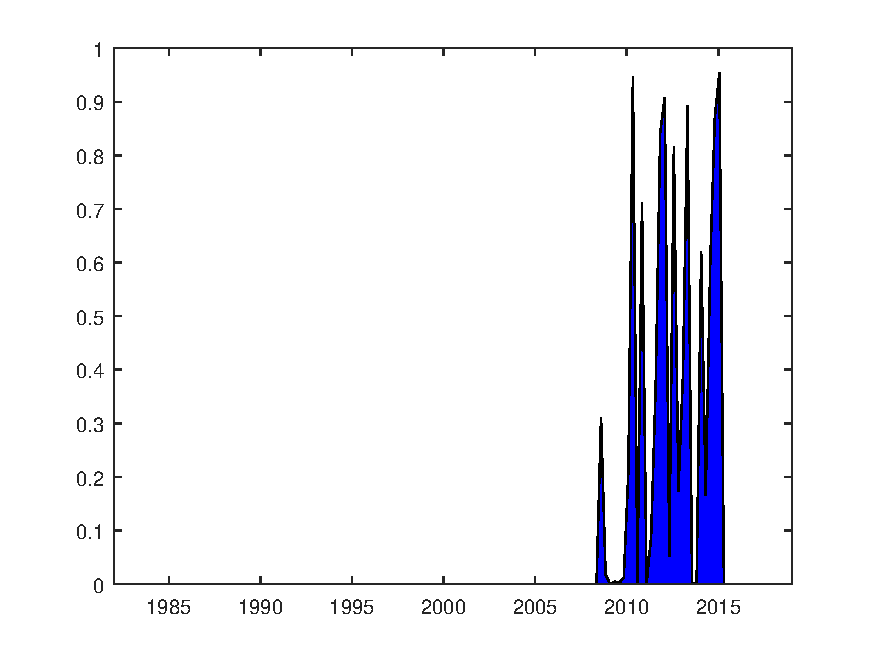
\includegraphics[scale=0.4]{figures/var1_4regime_regime3.pdf}}
\subfloat[Regime 4]{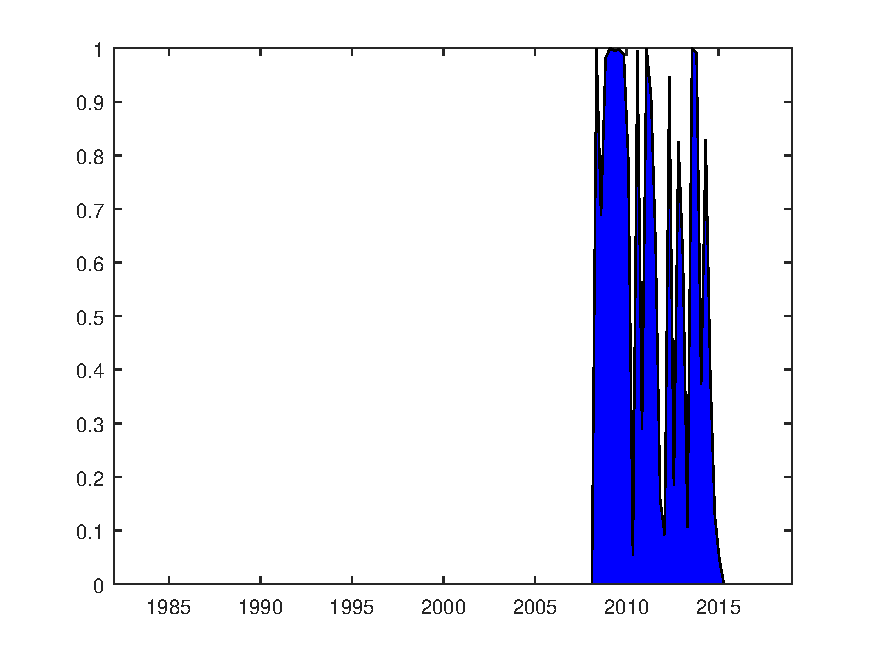
\includegraphics[scale=0.4]{figures/var1_4regime_regime4.pdf}}}
\caption{Estimated regime probabilities, VAR(1). }
\end{figure}


\begin{figure}[hbt!]
\centerline{\subfloat[Regime 1]{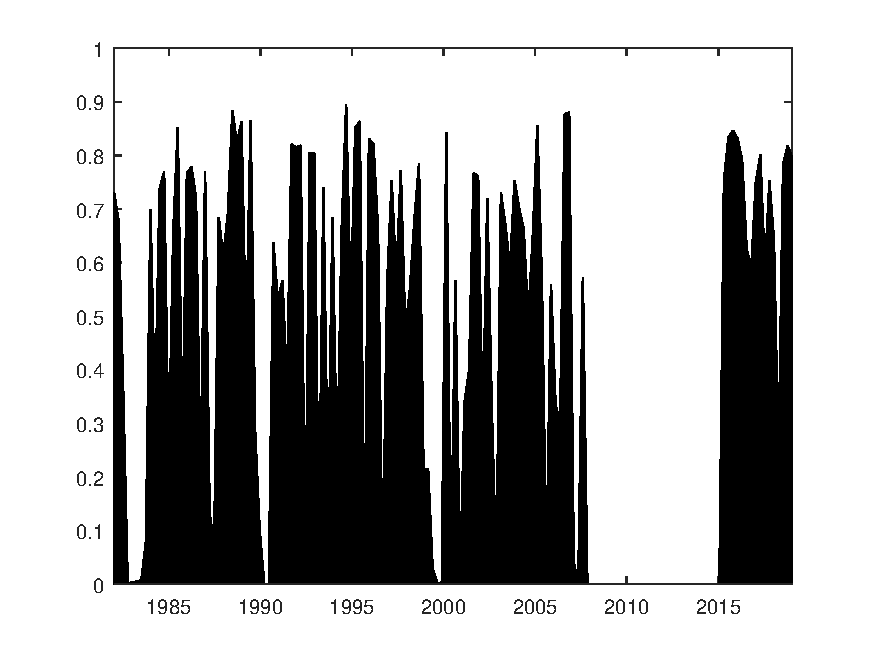
\includegraphics[scale=0.4]{figures/ar1_4regime_regime1.pdf}}
\subfloat[Regime 2]{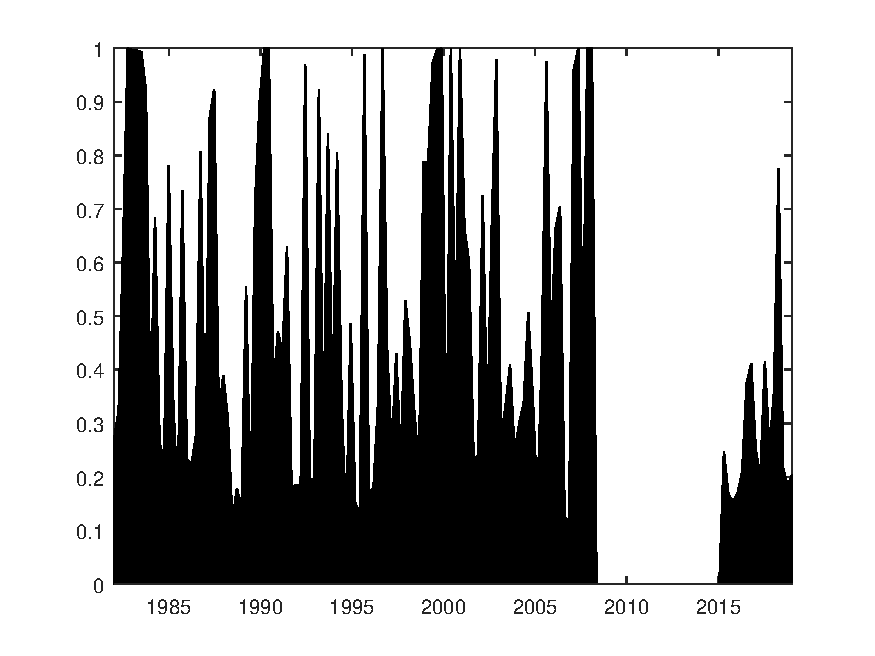
\includegraphics[scale=0.4]{figures/ar1_4regime_regime2.pdf}}}

\centerline{\subfloat[Regime 3]{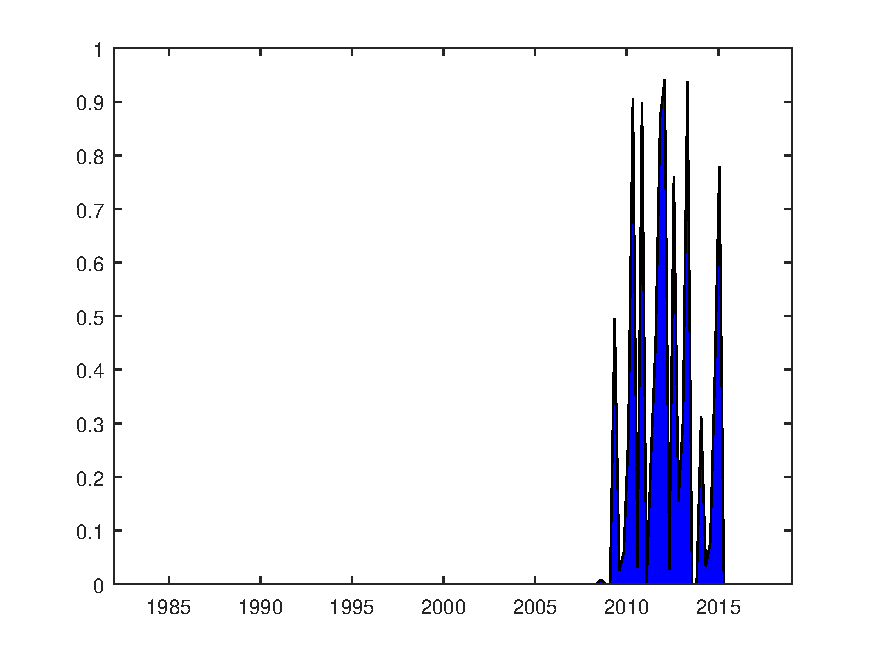
\includegraphics[scale=0.4]{figures/ar1_4regime_regime3.pdf}}
\subfloat[Regime 4]{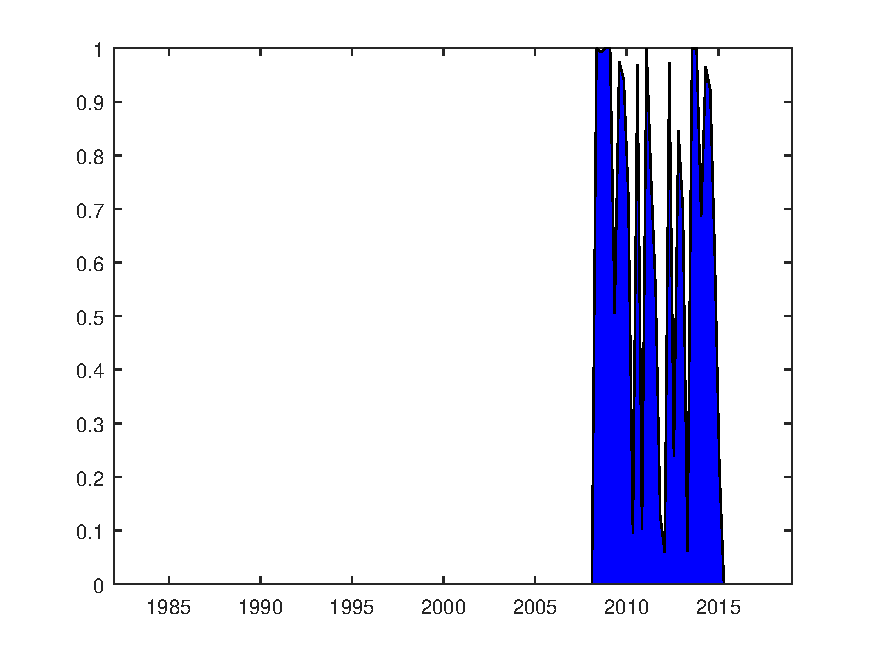
\includegraphics[scale=0.4]{figures/ar1_4regime_regime4.pdf}}}
\caption{Estimated regime probabilities, AR(1). }
\end{figure}



\begin{figure}[hbt!]
\centerline{
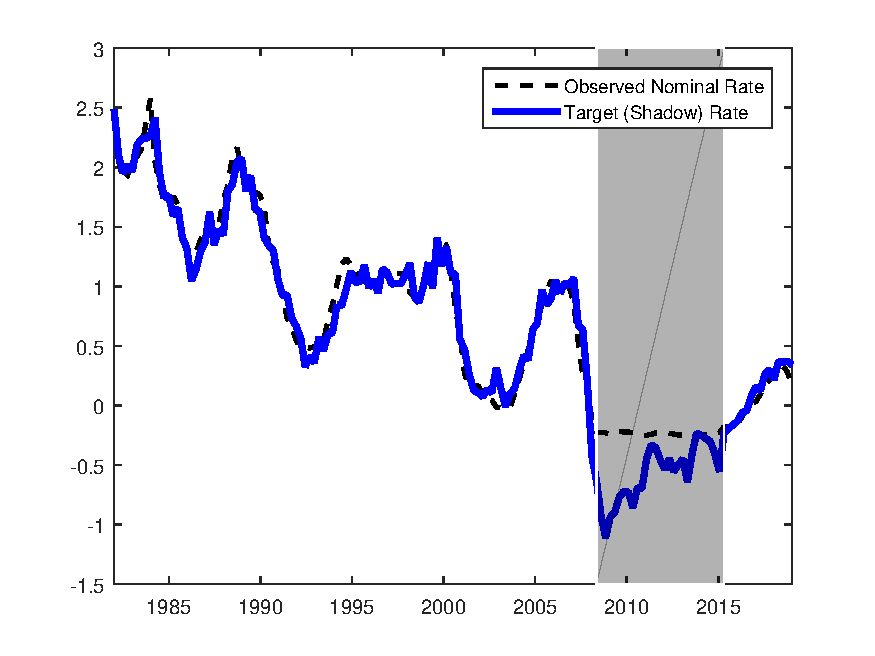
\includegraphics[scale=0.4]{figures/var1_4regime_shadowRate.pdf}
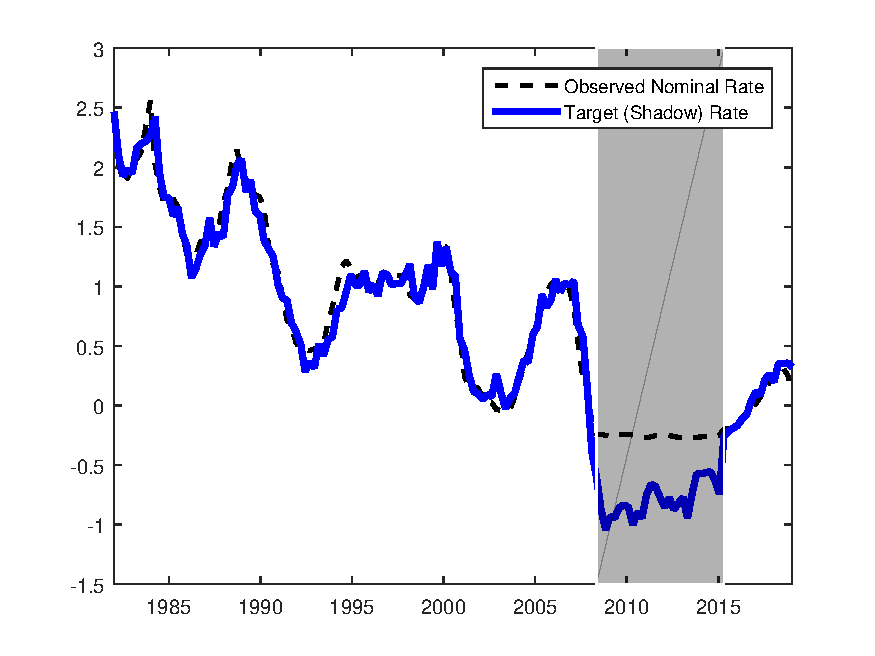
\includegraphics[scale=0.4]{figures/ar1_4regime_shadowRate.pdf}
}
\caption{Shadow rate along with the nominal interest rates in the 4-regime VAR(1) and AR(1) models. }
\end{figure}


\begin{table}[hbt!]
\begin{tabular}{l|l|l|l|l}
Regime Averages &  &  &  \\
\hline
 & Regime 1 & Regime 2 & Regime 3 & Regime 4 \\
Expectations & Learning & REE & Learning & REE \\
 &  &  &  & (Determinate Solution) \\
Monetary Policy & Taylor Rule & Taylor Rule & Passive & Passive \\
\hline
\hline
VAR(1) Learning&  &  &  &  \\
\hline
 Whole Period & 40.40\% & 40.30\% & 6.60\% & 11.90\% \\
 Normal Period & 50\% & 50\% & 0\% & 0\% \\
ZLB Period & 0\% & 0\% & 35.6\% & 64.3\% \\
\hline
\hline
AR(1) Learning&  &  &  &  \\
\hline
Whole Period & 41.40\% & 39.40\% & 5.94\% & 12.60\% \\
Normal Period & 51.2\% & 48.8\% & 0 & 0 \% \\
ZLB Period & 0\% & 0\% & 32\% & 68 \% \\ 
\end{tabular}
\end{table}

--time series of estimated alphas and betas
-estimated regime probabilities
-estimated n1 and n2 
-average p1 p2 p3 and p4 for both ar1 and ar2
-shadow rate together with nominal rate--plot only for VAR1-4regime, mention that its similar for AR1-4regime *(and also 2 regime models)
-impulse responses
--RISE IRFs (plot these similar to the previous paper, rather than as separate figures)
-plot all 4 learning models//both 2 regime and 4 regime 
-which IRFs??--to be decided. Most likely only output gap

\FloatBarrier

\subsection{Conditional Impulse Responses}


\begin{figure}[hbt!]

\subfloat[VAR(1), 4-regime]{
{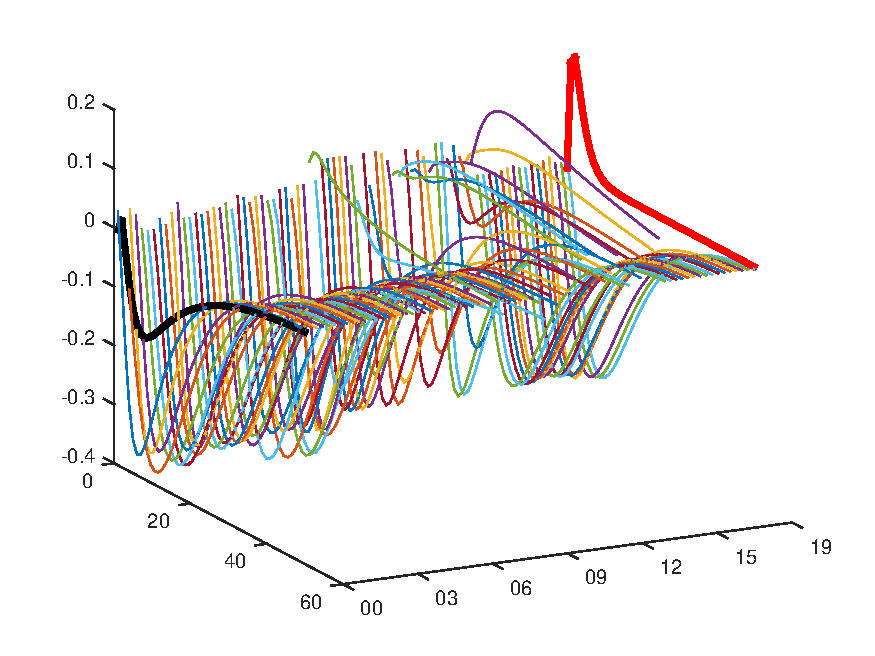
\includegraphics[scale=0.3]{figures/var1_4reg_3d_IRF_y_etaPi}}
{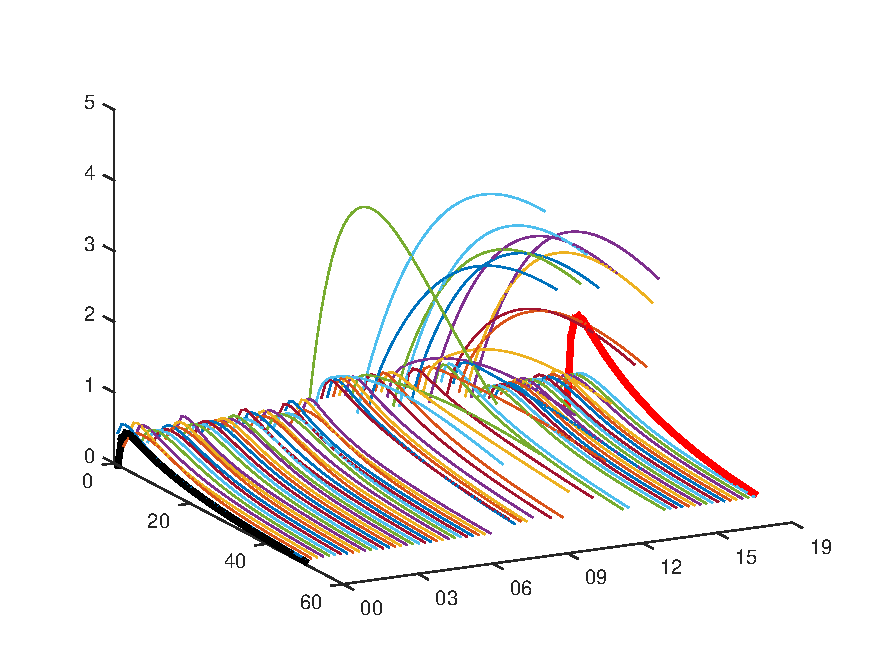
\includegraphics[scale=0.3]{figures/var1_4reg_3d_IRF_y_etaY}}
{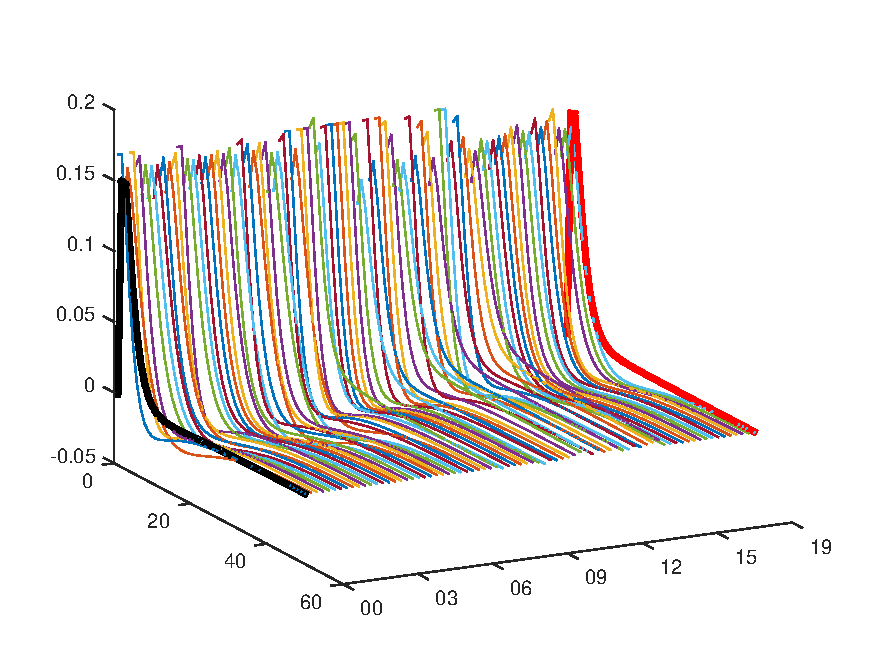
\includegraphics[scale=0.3]{figures/var1_4reg_3d_IRF_pi_etaPi}}
{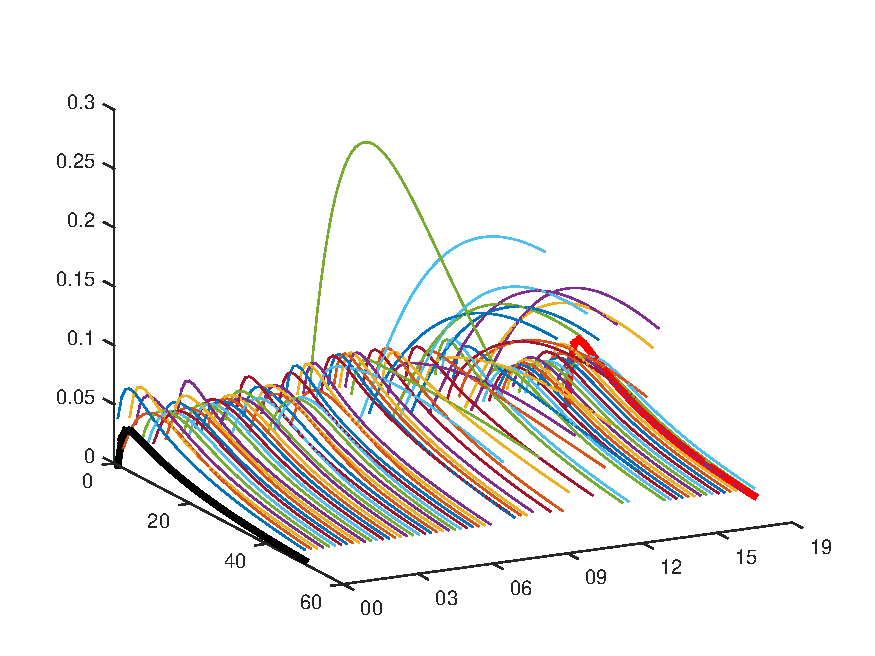
\includegraphics[scale=0.3]{figures/var1_4reg_3d_IRF_pi_etaY}}}

\subfloat[AR(1), 4-regime]{
{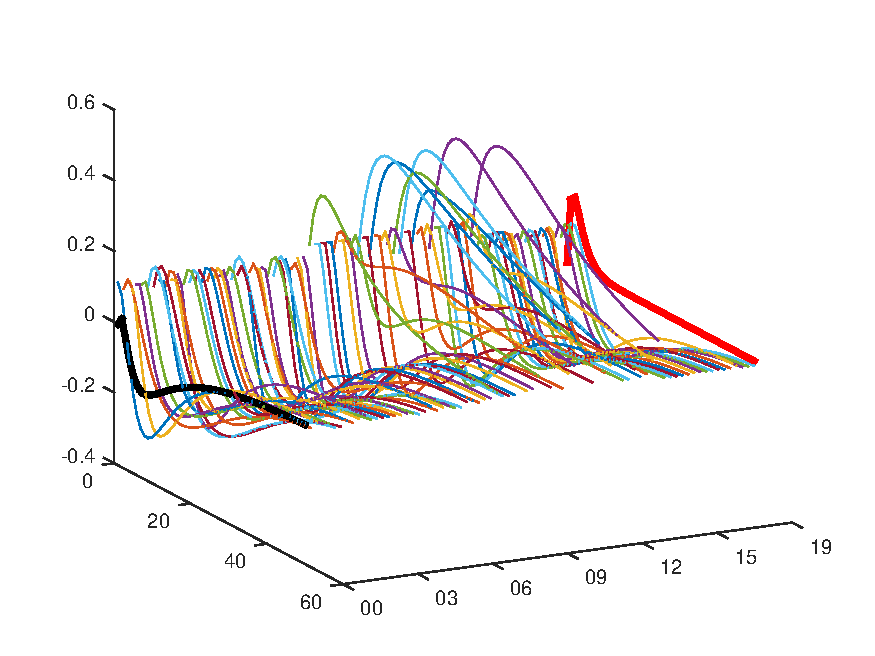
\includegraphics[scale=0.3]{figures/ar1_4reg_3d_IRF_y_etaPi}}
{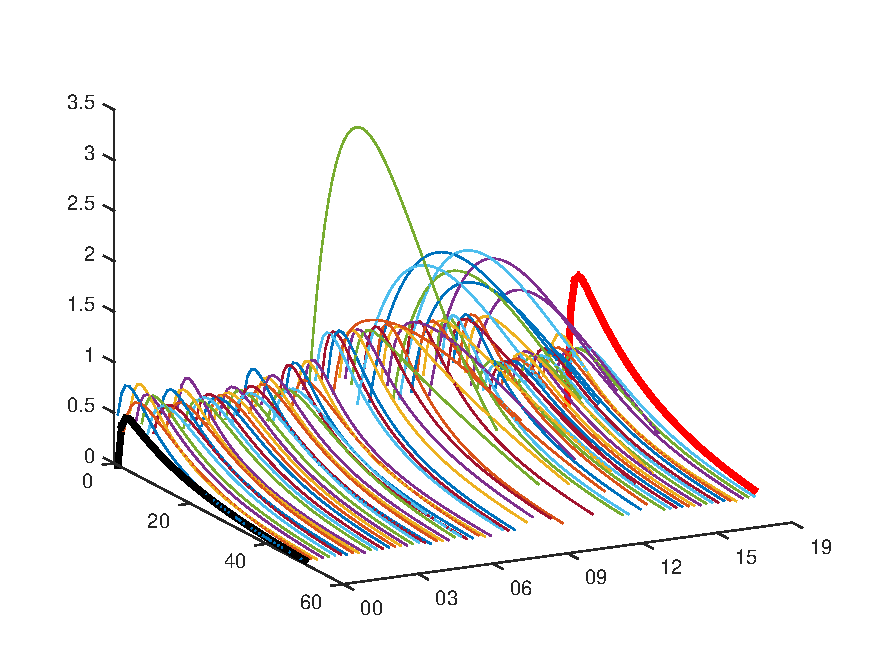
\includegraphics[scale=0.3]{figures/ar1_4reg_3d_IRF_y_etaY}}
{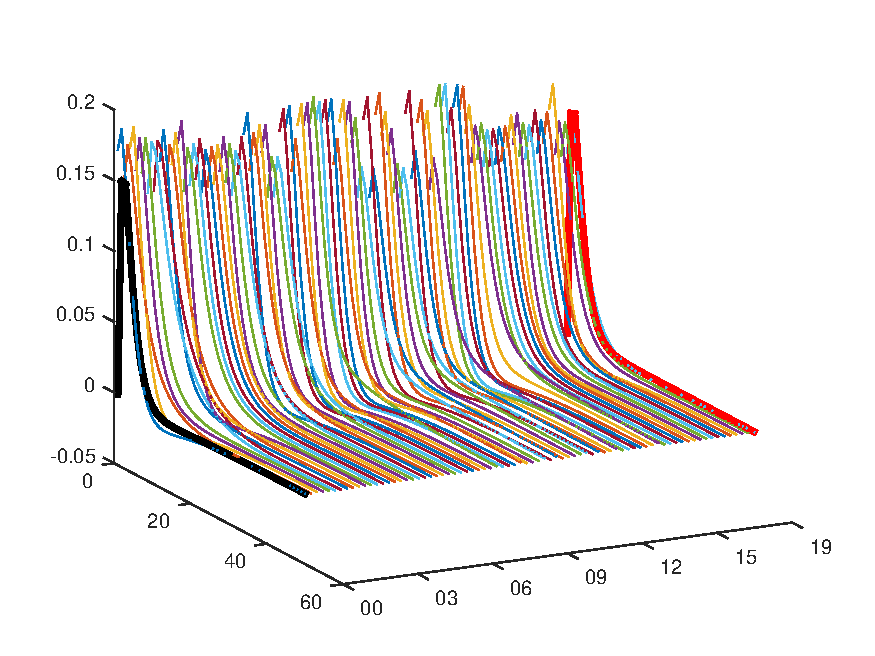
\includegraphics[scale=0.3]{figures/ar1_4reg_3d_IRF_pi_etaPi}}
{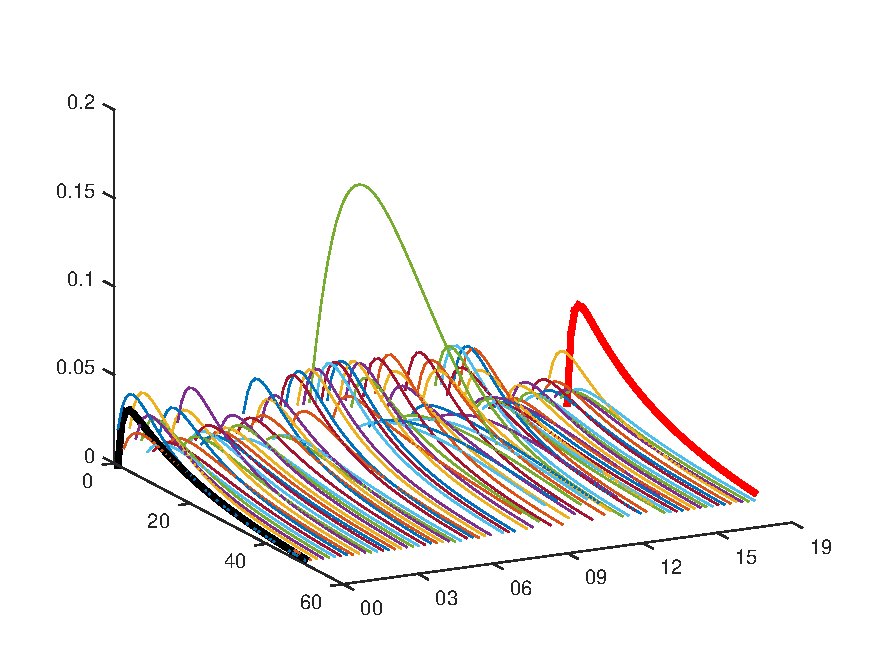
\includegraphics[scale=0.3]{figures/ar1_4reg_3d_IRF_pi_etaY}}}


\subfloat[VAR(1), 2-regime]{
{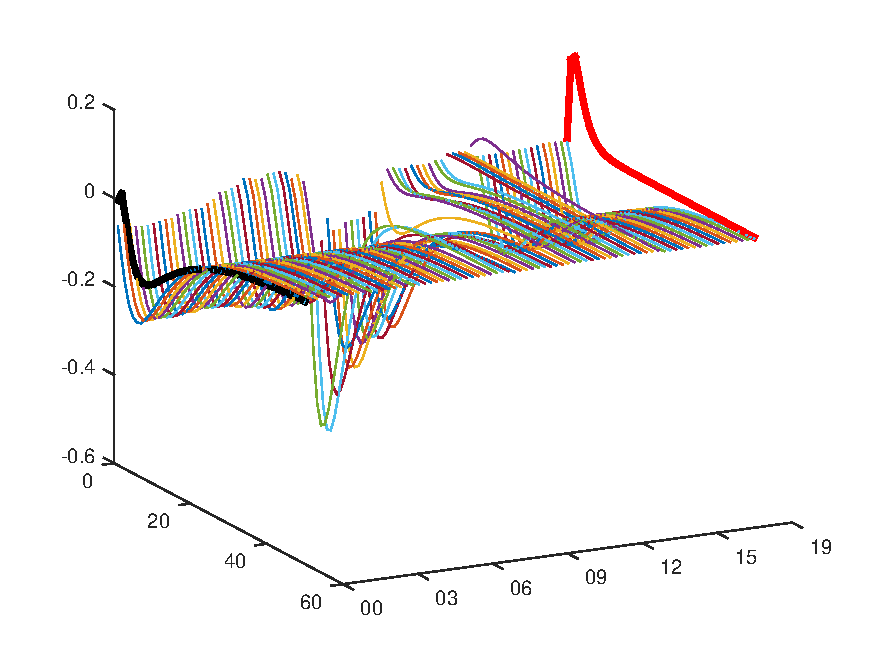
\includegraphics[scale=0.3]{figures/var1_2reg_3d_IRF_y_etaPi}}
{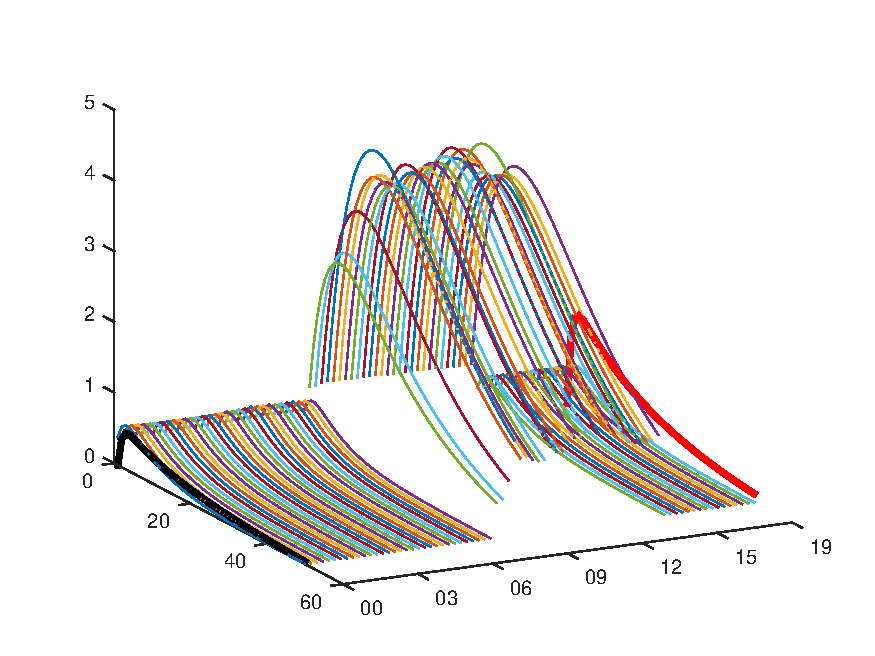
\includegraphics[scale=0.3]{figures/var1_2reg_3d_IRF_y_etaY}}
{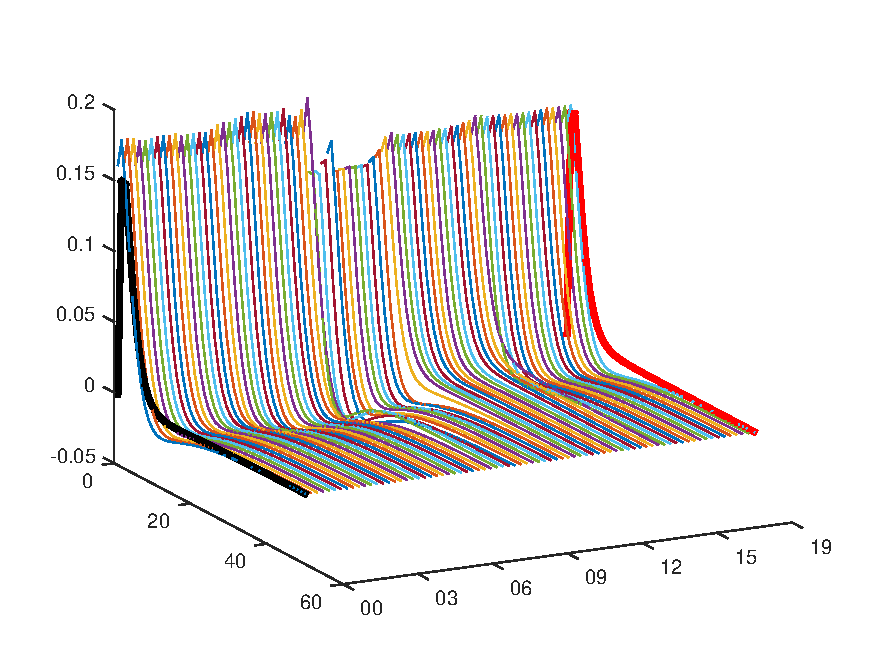
\includegraphics[scale=0.3]{figures/var1_2reg_3d_IRF_pi_etaPi}}
{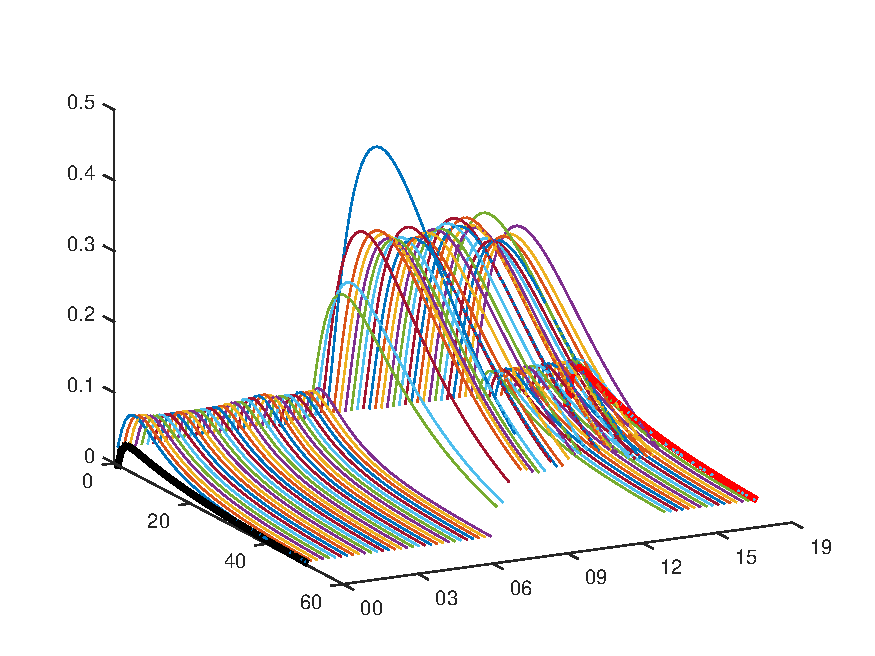
\includegraphics[scale=0.3]{figures/var1_2reg_3d_IRF_pi_etaY}}}


\subfloat[AR(1), 2-regime]{
{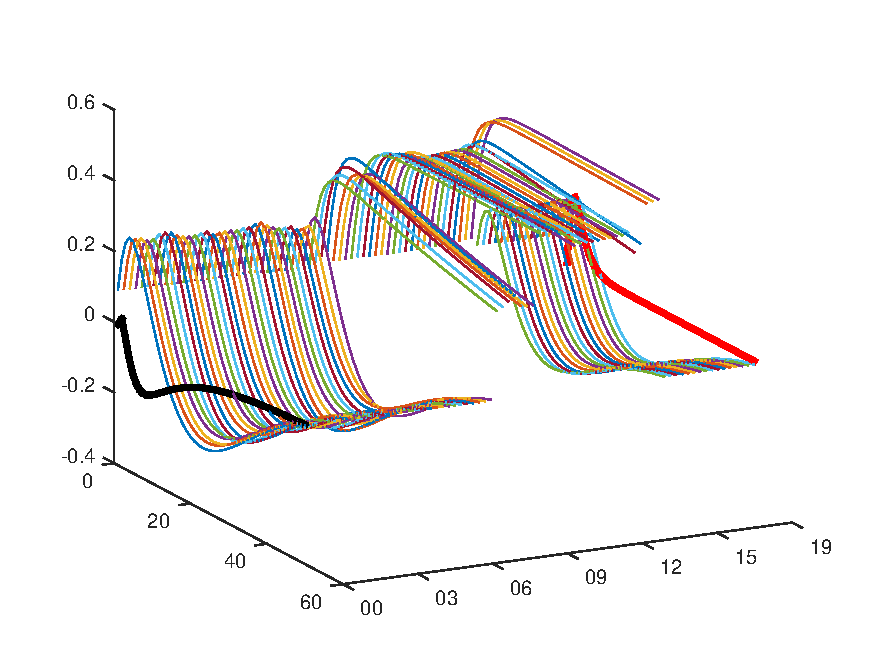
\includegraphics[scale=0.3]{figures/ar1_2reg_3d_IRF_y_etaPi}}
{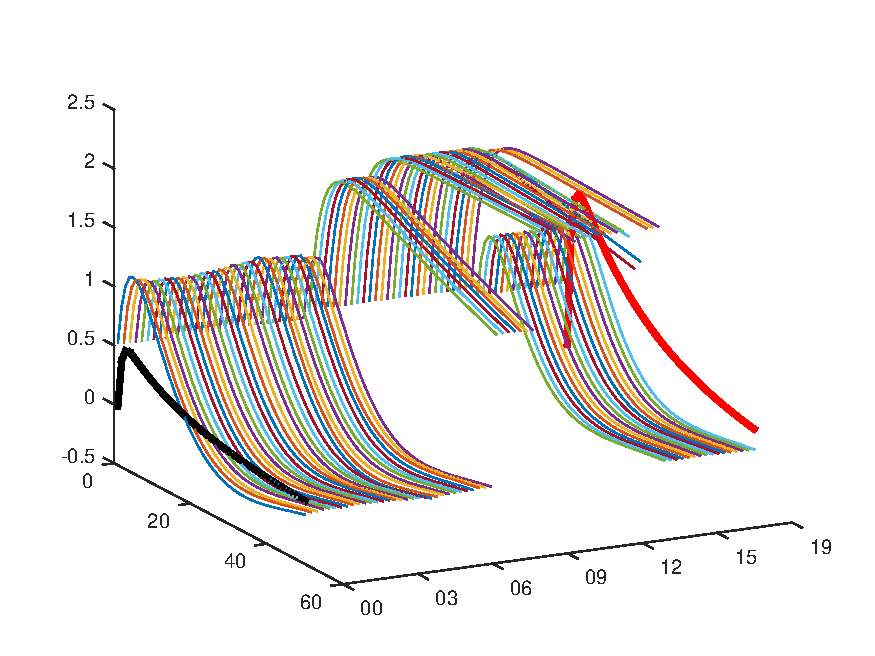
\includegraphics[scale=0.3]{figures/ar1_2reg_3d_IRF_y_etaY}}
{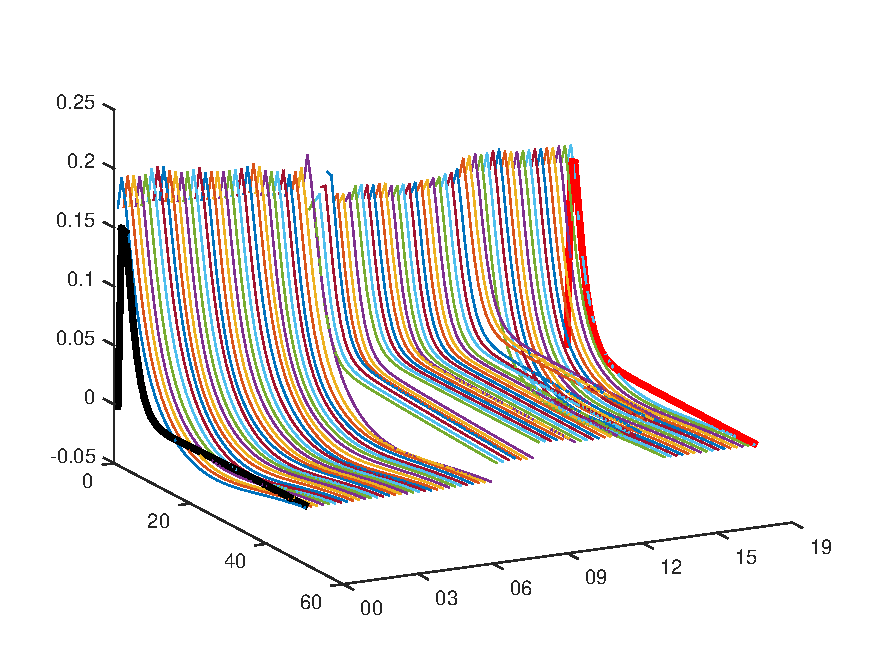
\includegraphics[scale=0.3]{figures/ar1_2reg_3d_IRF_pi_etaPi}}
{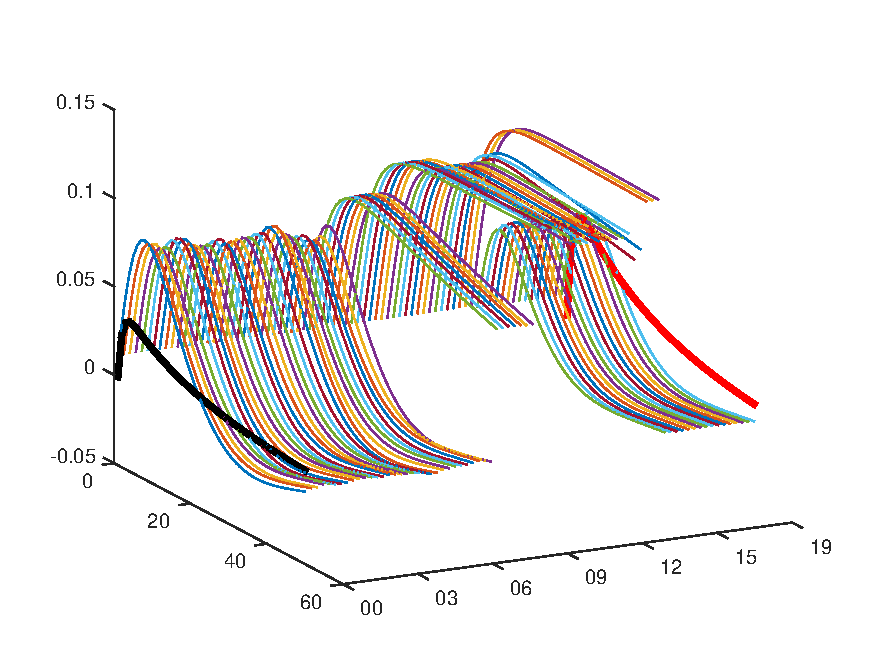
\includegraphics[scale=0.3]{figures/ar1_2reg_3d_IRF_pi_etaY}}}

\caption{Conditional impulse responses for VAR(1) and AR(1) learning models.}
\end{figure}


\begin{figure}[hbt!]

\subfloat[VAR(1), 4-regime]{
{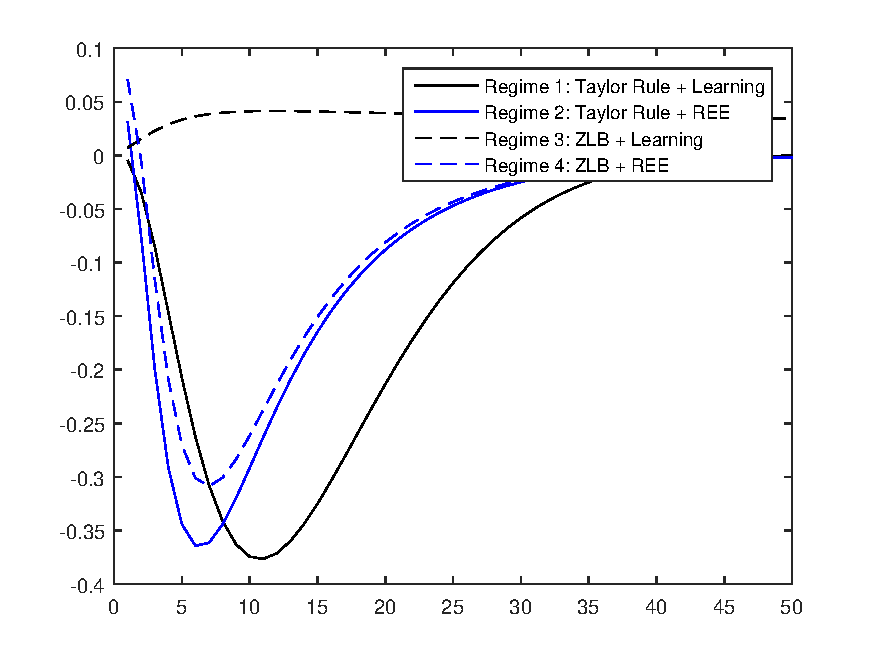
\includegraphics[scale=0.3]{figures/var1_4reg_averageIRF_y_etaPi}}
{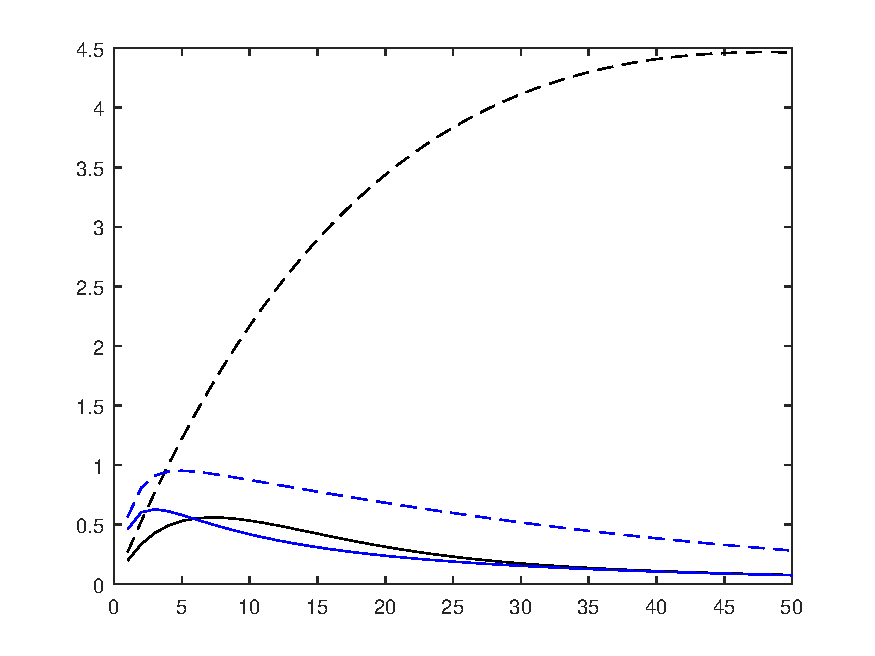
\includegraphics[scale=0.3]{figures/var1_4reg_averageIRF_y_etaY}}
{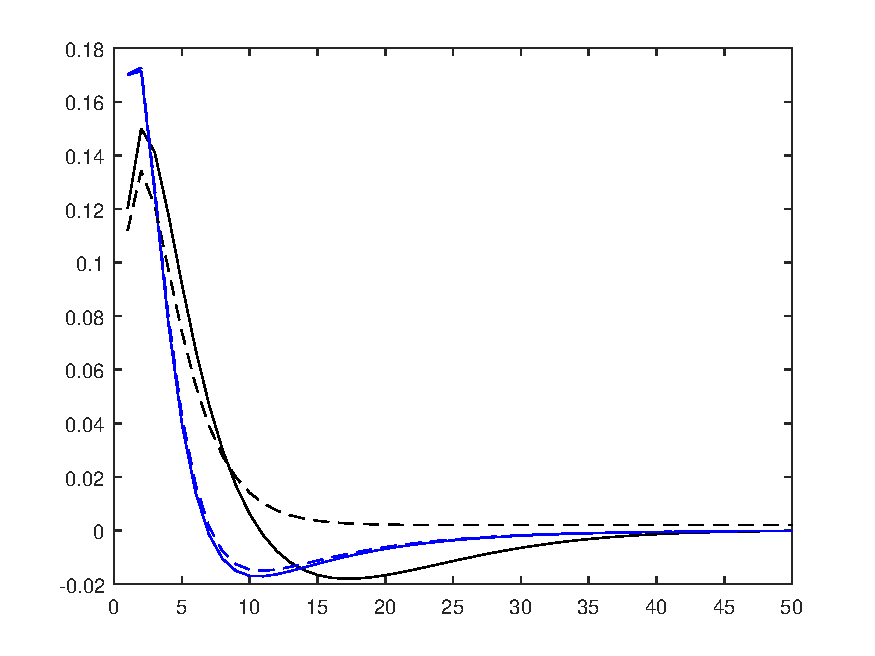
\includegraphics[scale=0.3]{figures/var1_4reg_averageIRF_pi_etaPi}}
{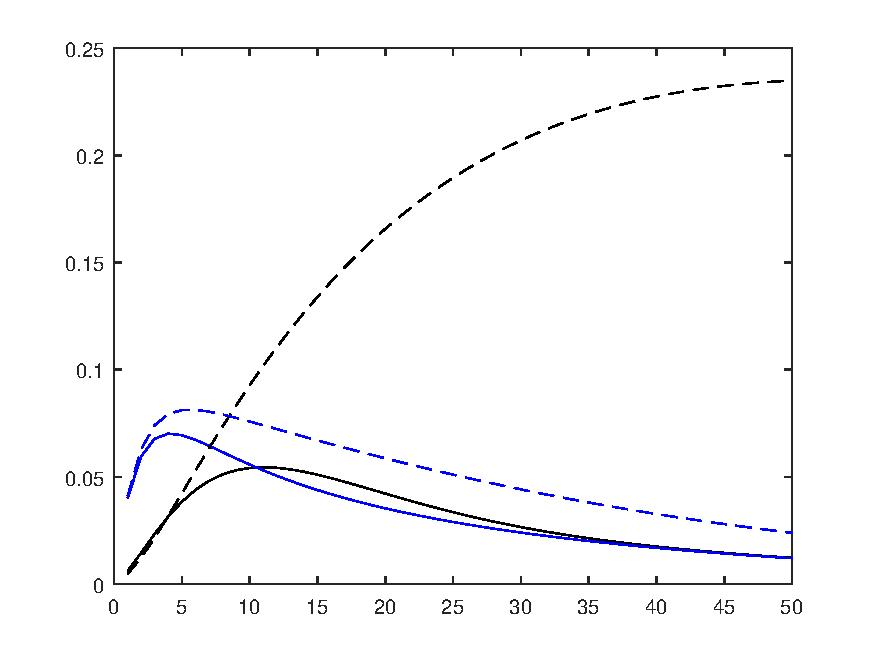
\includegraphics[scale=0.3]{figures/var1_4reg_averageIRF_pi_etaY}}}

\subfloat[AR(1), 4-regime]{
{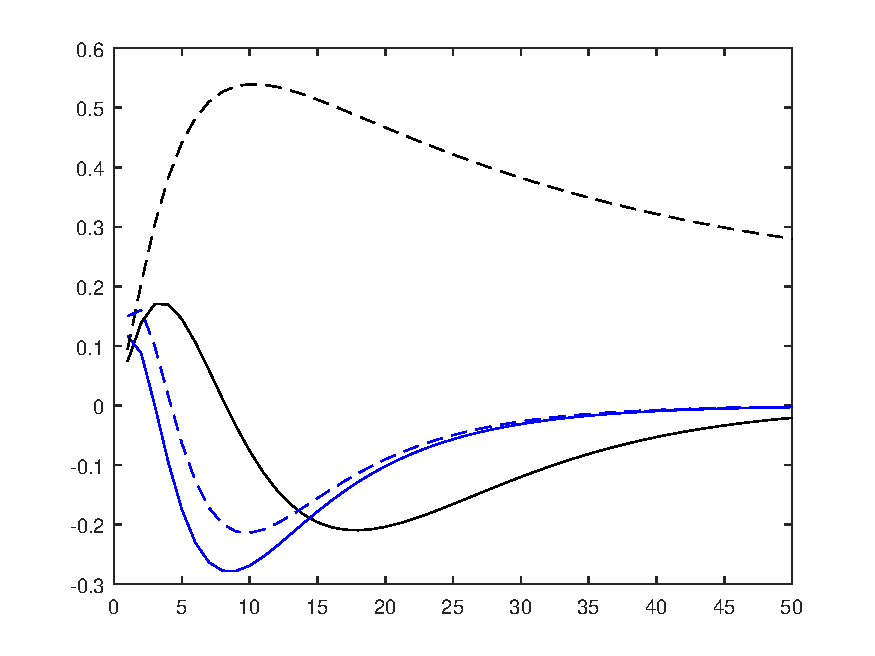
\includegraphics[scale=0.3]{figures/ar1_4reg_averageIRF_y_etaPi}}
{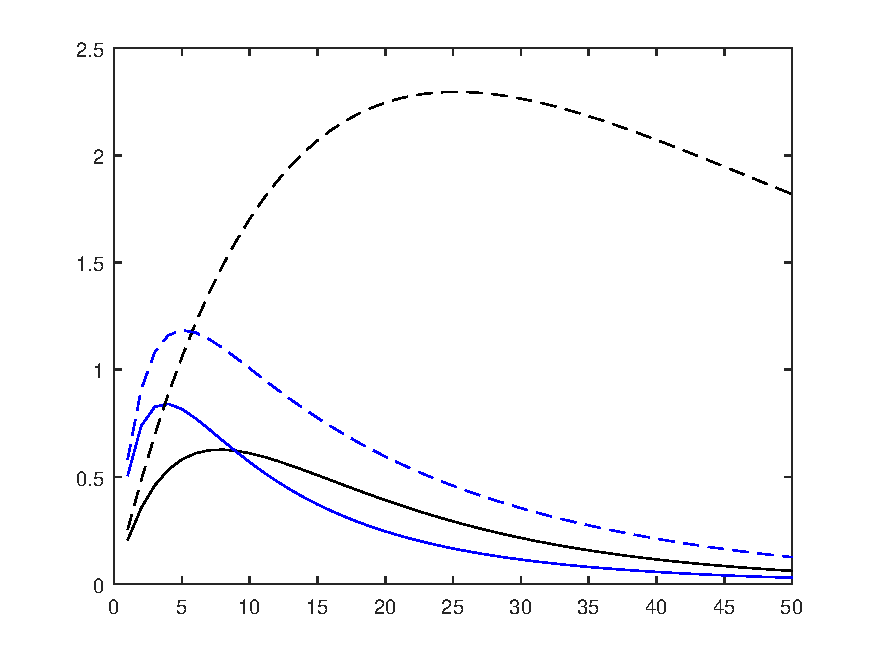
\includegraphics[scale=0.3]{figures/ar1_4reg_averageIRF_y_etaY}}
{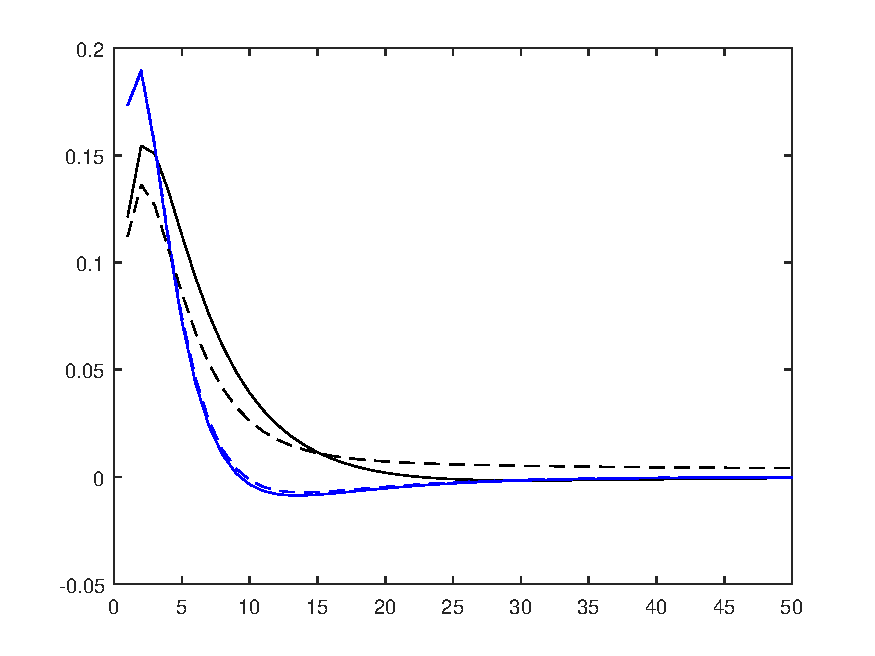
\includegraphics[scale=0.3]{figures/ar1_4reg_averageIRF_pi_etaPi}}
{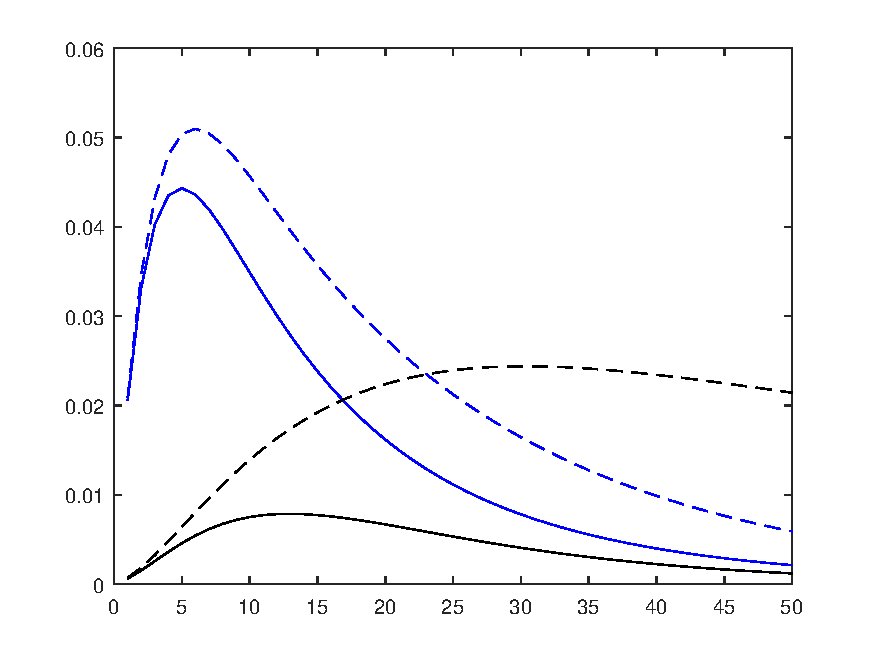
\includegraphics[scale=0.3]{figures/ar1_4reg_averageIRF_pi_etaY}}}

\subfloat[VAR(1), 2-regime]{
{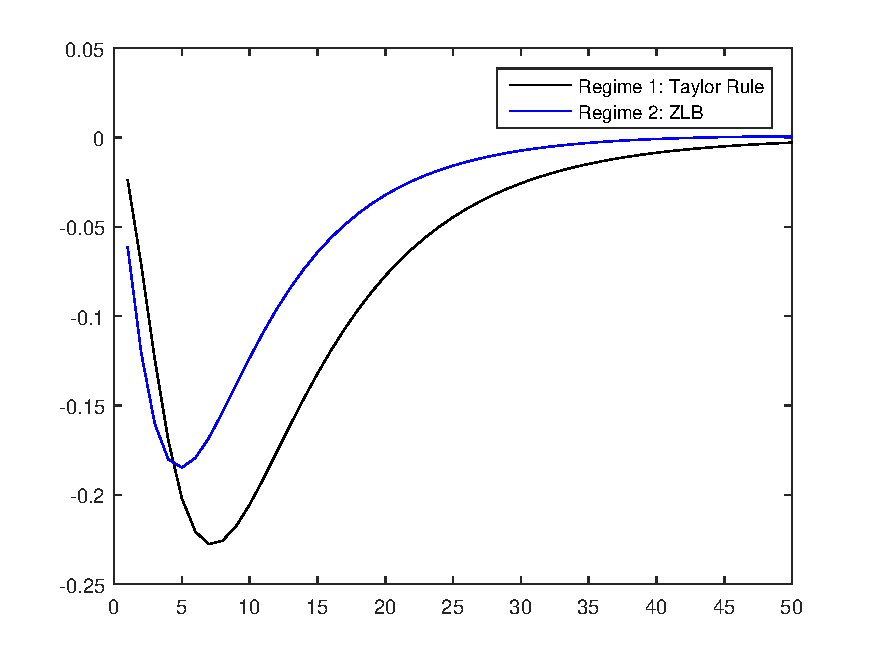
\includegraphics[scale=0.3]{figures/var1_2reg_averageIRF_y_etaPi}}
{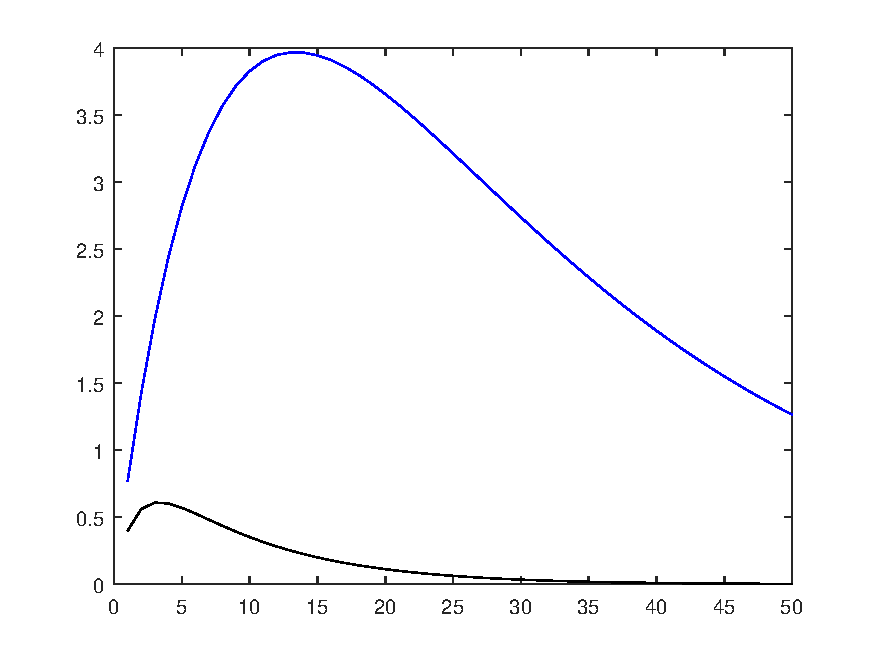
\includegraphics[scale=0.3]{figures/var1_2reg_averageIRF_y_etaY}}
{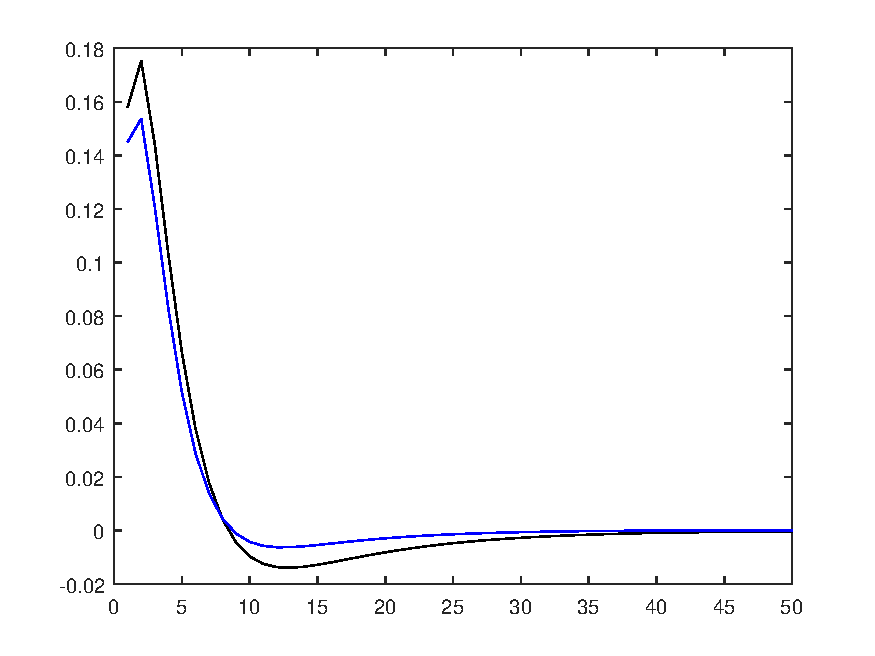
\includegraphics[scale=0.3]{figures/var1_2reg_averageIRF_pi_etaPi}}
{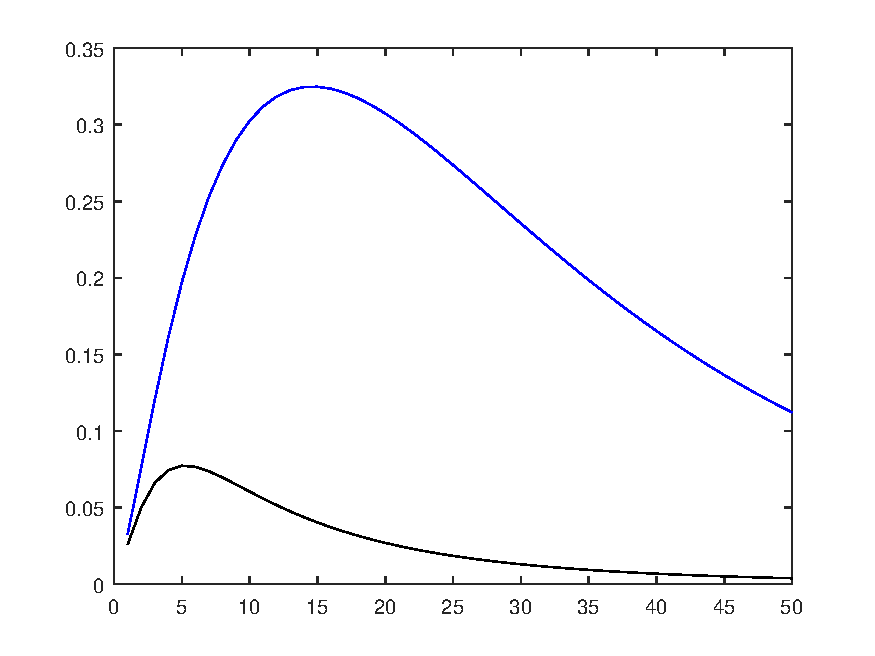
\includegraphics[scale=0.3]{figures/var1_2reg_averageIRF_pi_etaY}}}

\subfloat[AR(1), 2-regime]{
{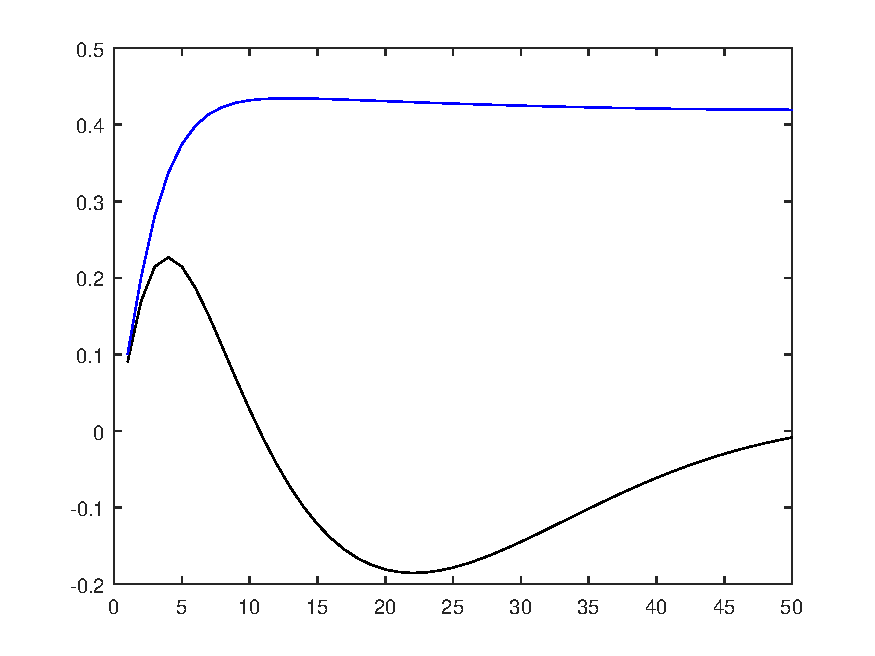
\includegraphics[scale=0.3]{figures/ar1_2reg_averageIRF_y_etaPi}}
{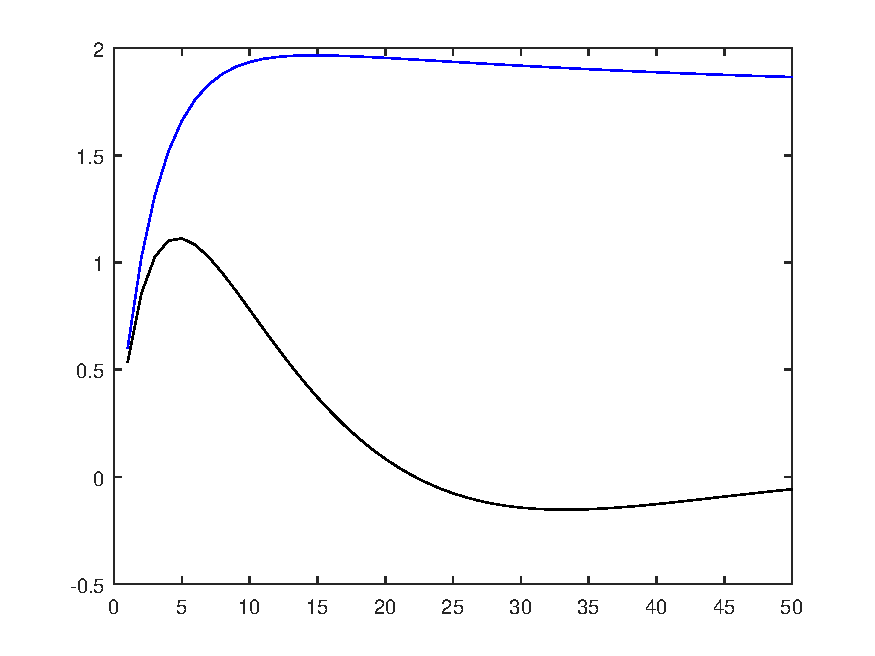
\includegraphics[scale=0.3]{figures/ar1_2reg_averageIRF_y_etaY}}
{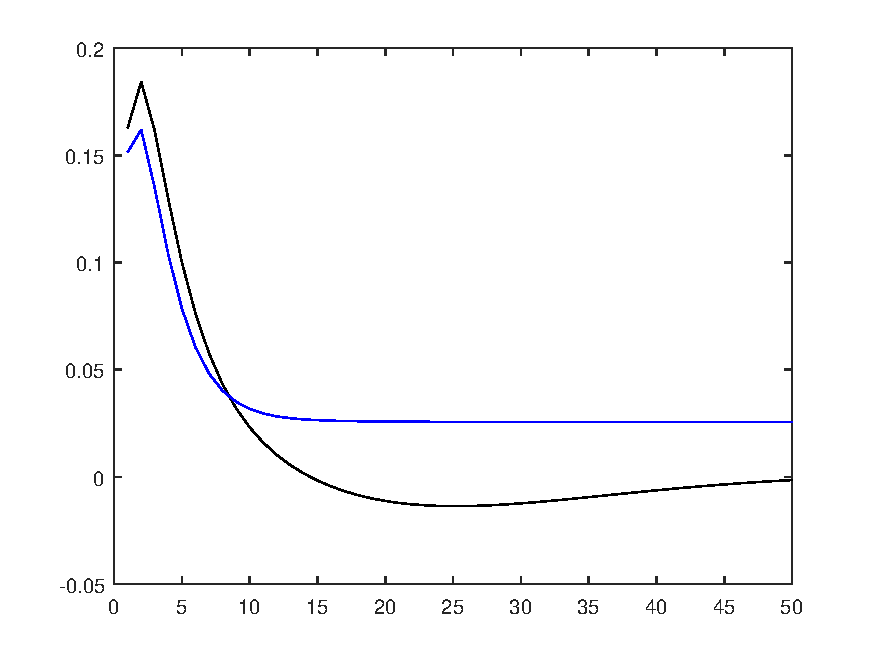
\includegraphics[scale=0.3]{figures/ar1_2reg_averageIRF_pi_etaPi}}
{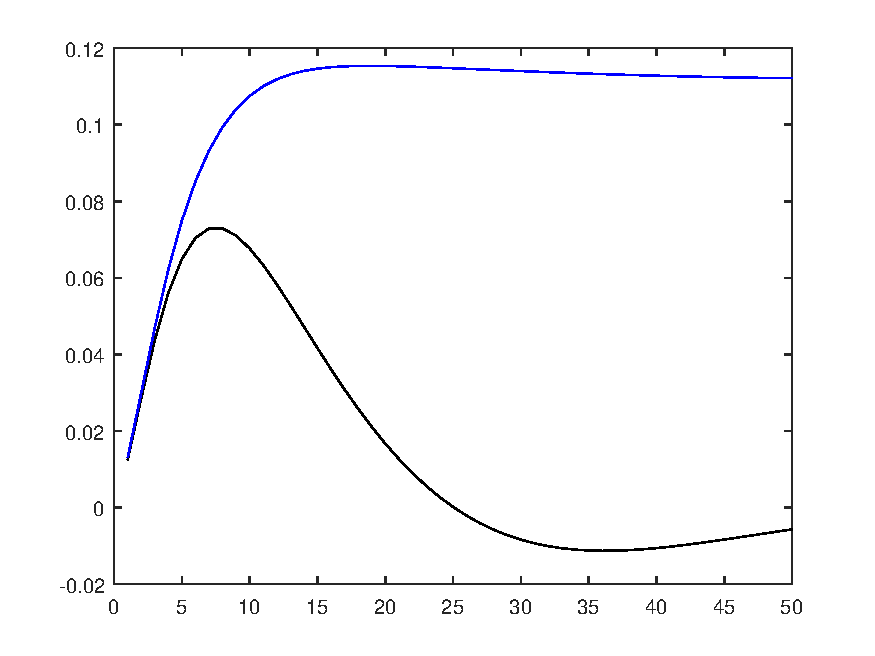
\includegraphics[scale=0.3]{figures/ar1_2reg_averageIRF_pi_etaY}}}

\caption{Average impulse responses for VAR(1) and AR(1) learning models. }
\end{figure}



\FloatBarrier

\section{Counterfactual Experiments and Monte Carlo Simulations}

\subsection{Counterfactual I: Estimated shocks, different fractions}



\begin{figure}[hbt!]

\centerline{
\subfloat[Output gap]{
{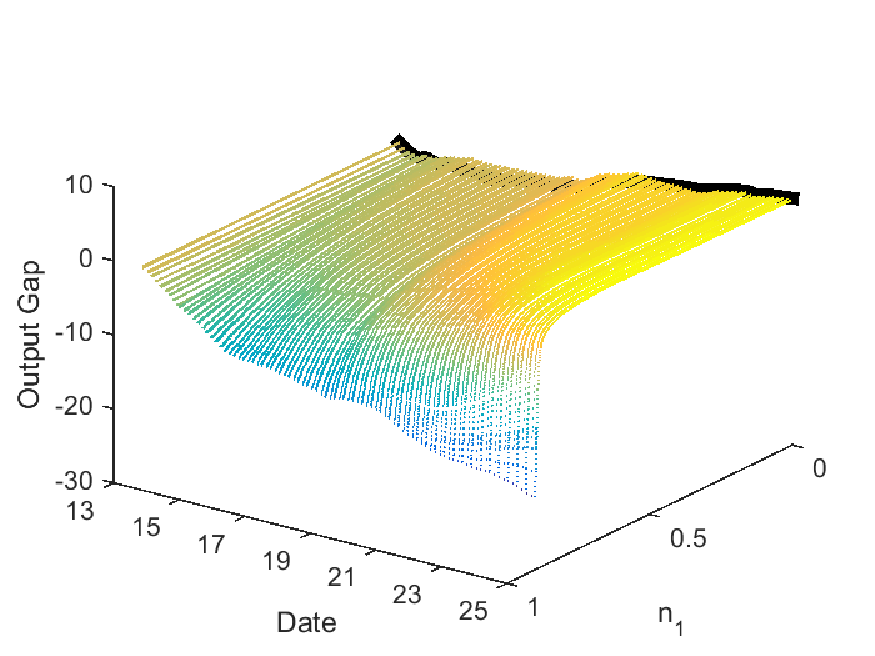
\includegraphics[scale=0.4]{figures/var1_CF1_fixedShocks_gap}}
{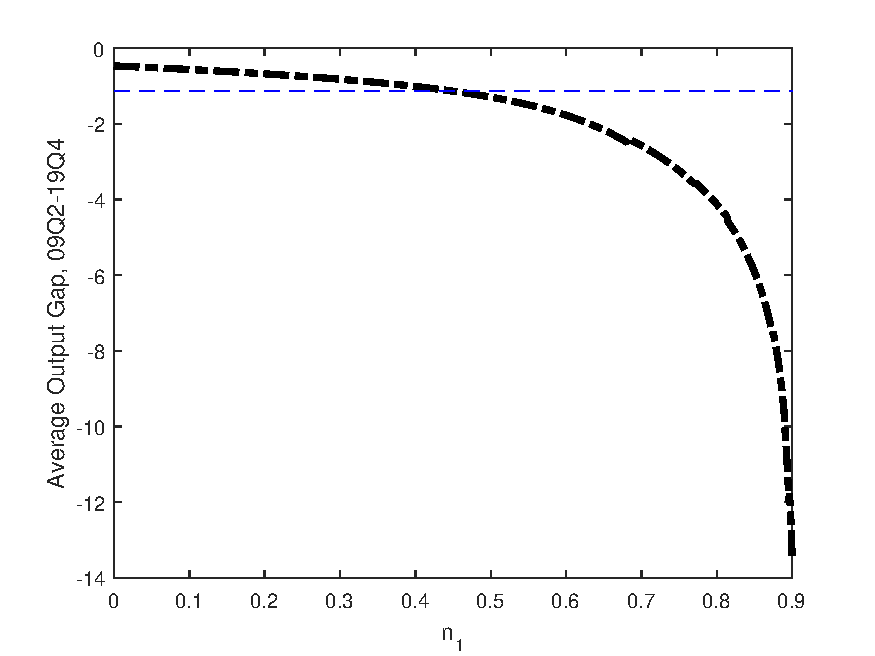
\includegraphics[scale=0.4]{figures/var1_CF1_fixedShocks_gapMean}}}
}

\centerline{
\subfloat[Inflation]{
{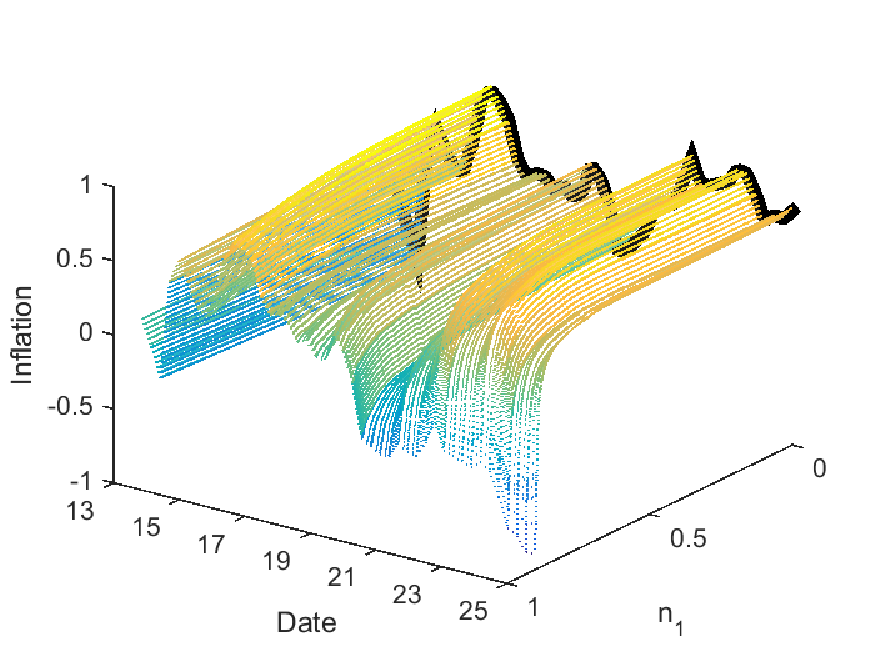
\includegraphics[scale=0.4]{figures/var1_CF1_fixedShocks_pi}}
{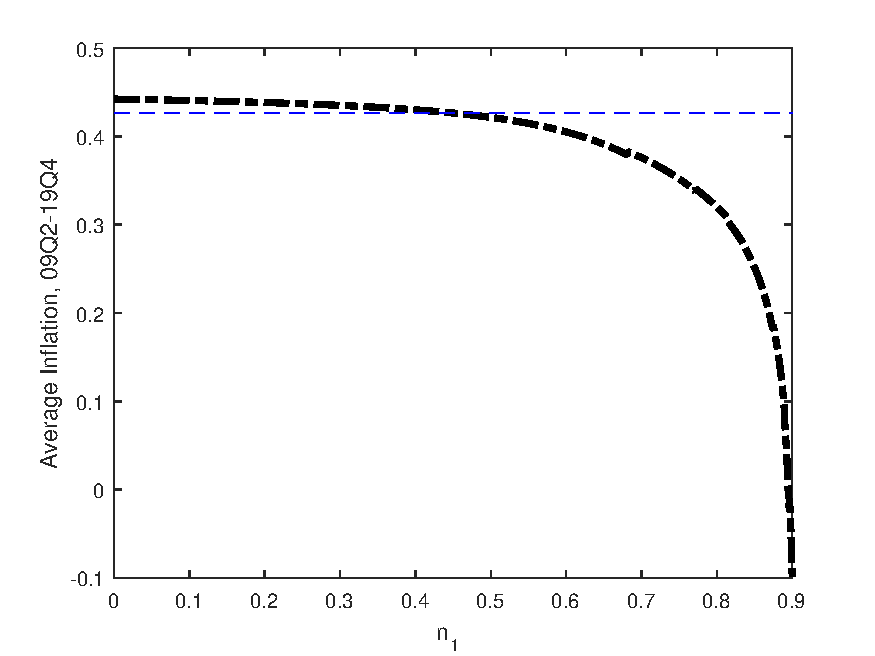
\includegraphics[scale=0.4]{figures/var1_CF1_fixedShocks_piMean}}}
}


\centerline{
\subfloat[Shadow Rate]{
{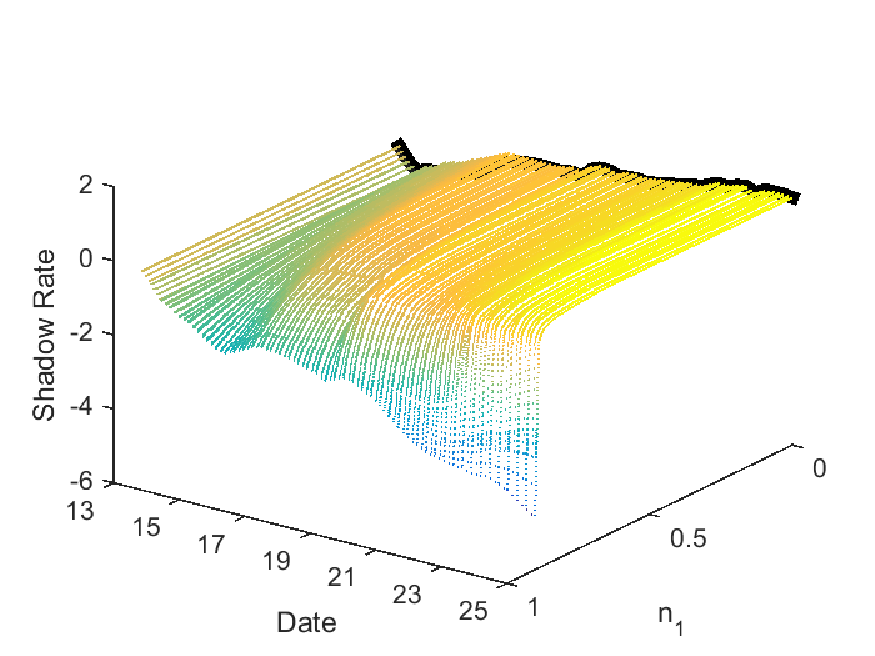
\includegraphics[scale=0.4]{figures/var1_CF1_fixedShocks_SR}}
{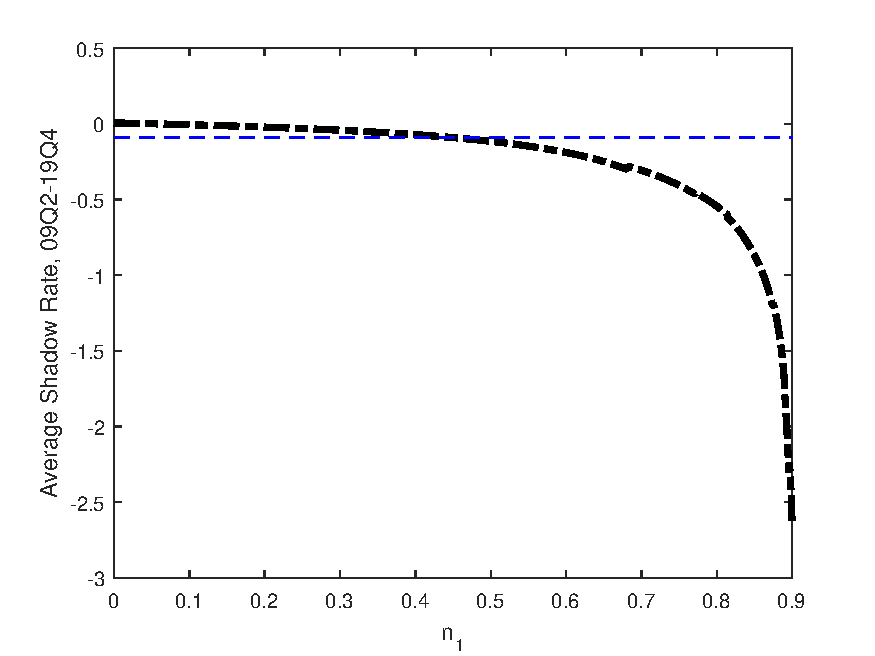
\includegraphics[scale=0.4]{figures/var1_CF1_fixedShocks_SRMean}}}
}


\centerline{
\subfloat[Taylor Rule Probability]{
{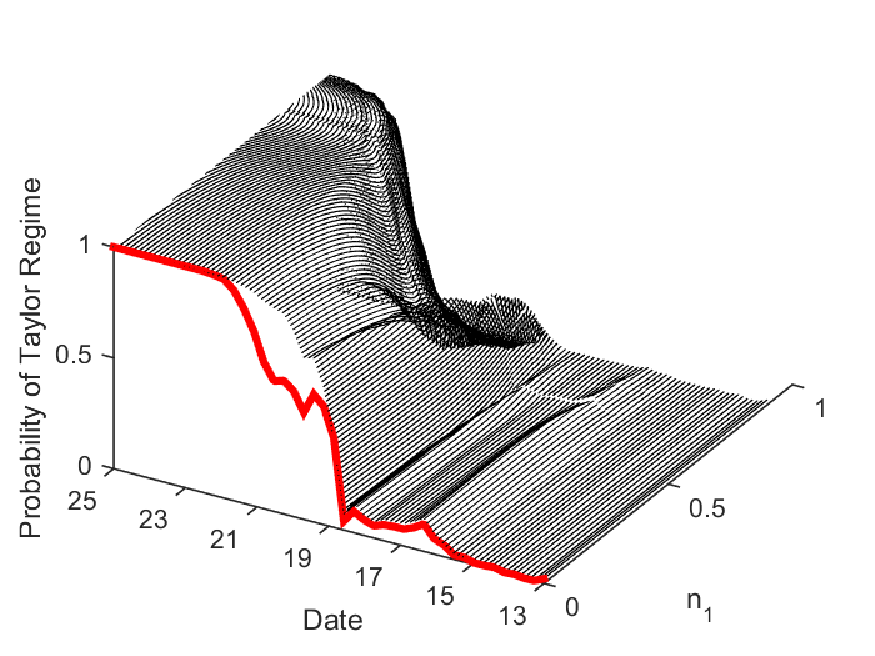
\includegraphics[scale=0.4]{figures/var1_CF1_fixedShocks_probTaylor}}
{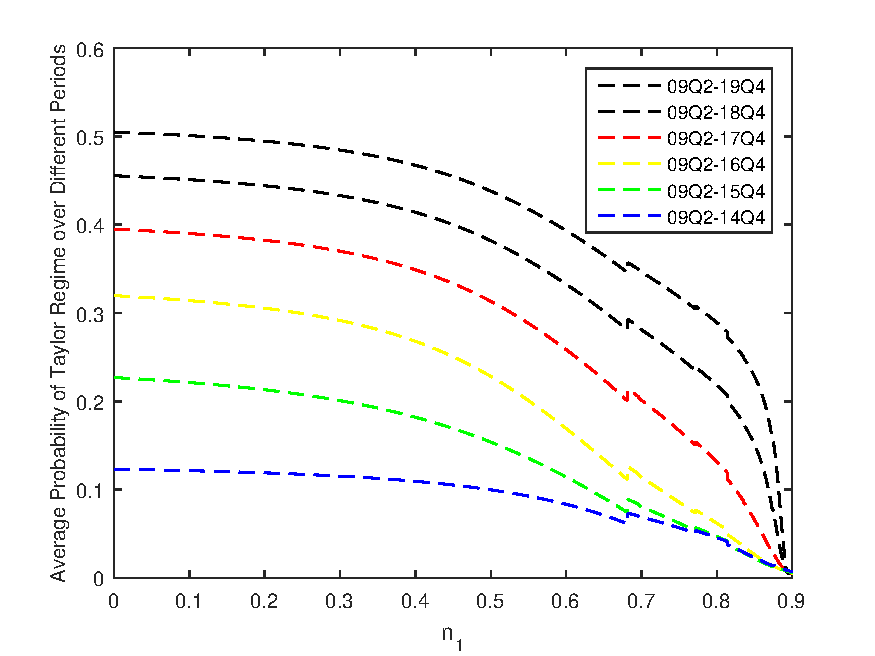
\includegraphics[scale=0.4]{figures/var1_CF1_fixedShocks_probTaylorMean}}}
}

\caption{Period-specific time paths (left)and averages over the counterfactual period (right).}
\end{figure}


\FloatBarrier

\subsection{Counterfactual II: Estimated shocks, different fractions and gain values (only averages)}
\begin{figure}[h]
\centerline{
\subfloat[Output Gap]{{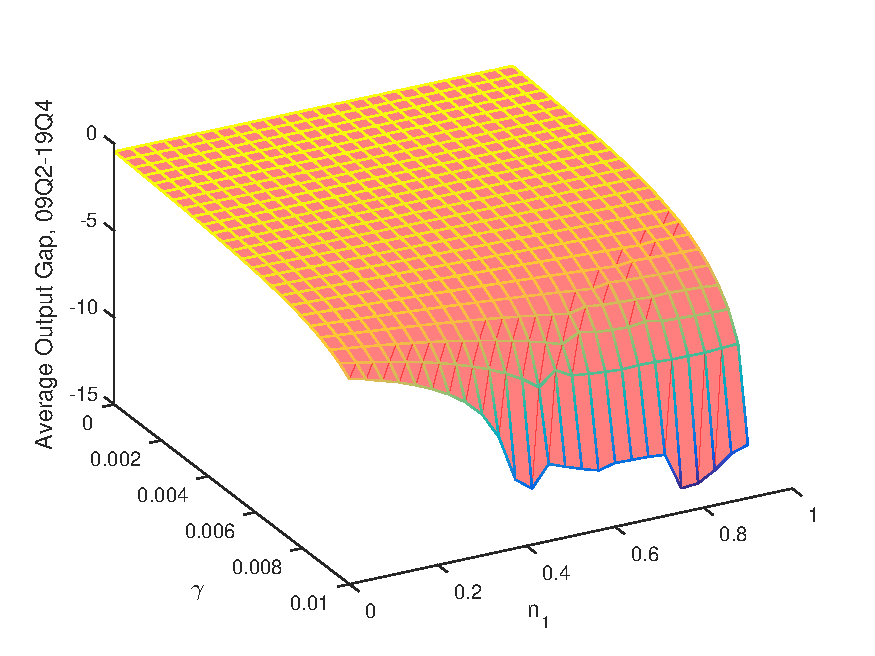
\includegraphics[scale=0.35]{figures/var1_CF2_fixedShocks_gap}}}
\subfloat[Inflation]{{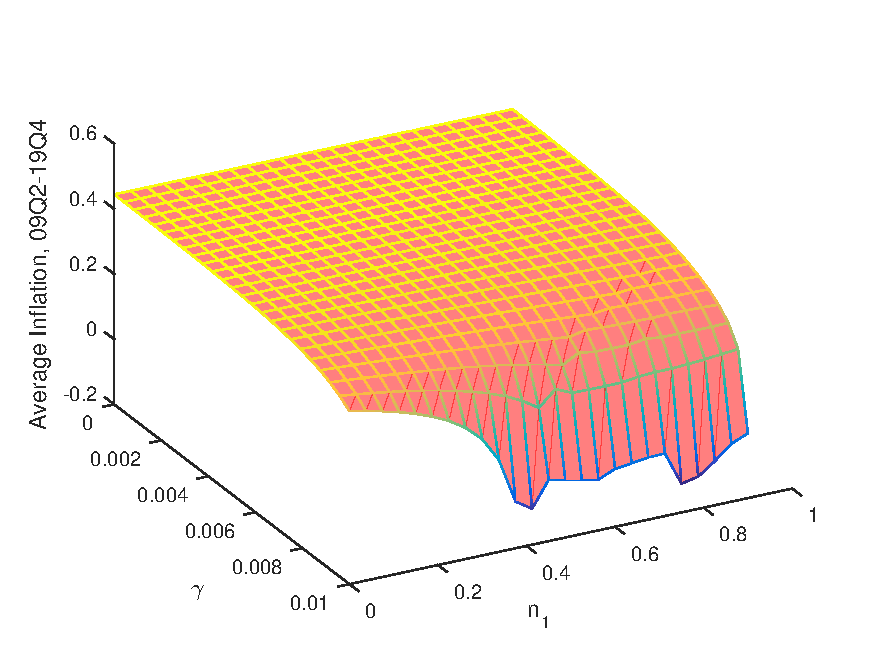
\includegraphics[scale=0.35]{figures/var1_CF2_fixedShocks_pi}}}
\subfloat[Shadow Rate]{{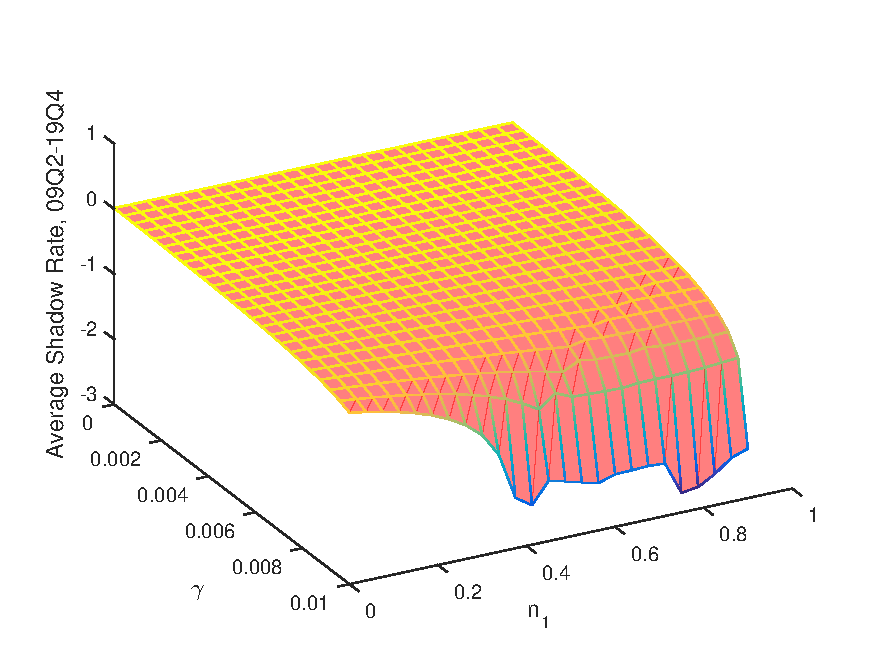
\includegraphics[scale=0.35]{figures/var1_CF2_fixedShocks_SR}}}
}
\end{figure}

\FloatBarrier

\subsection{Counterfactual III: Randomized Shocks, post 2019Q4 period}

\begin{figure}[hbt!]
\centerline{
\subfloat[Output Gap]{{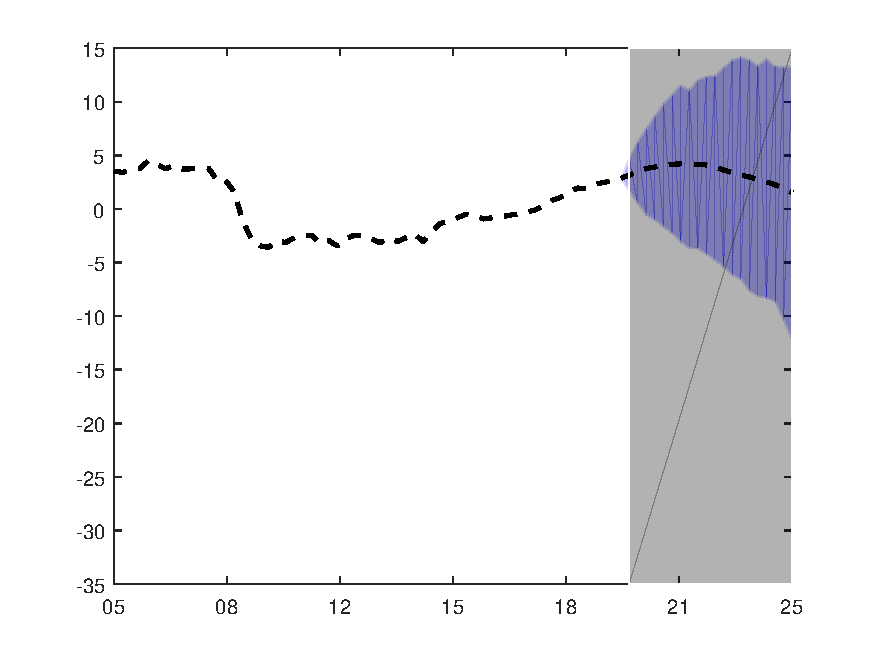
\includegraphics[scale=0.55]{figures/var1_CF3_randomShocks1_normalReg_gap}}}
\subfloat[Inflation]{{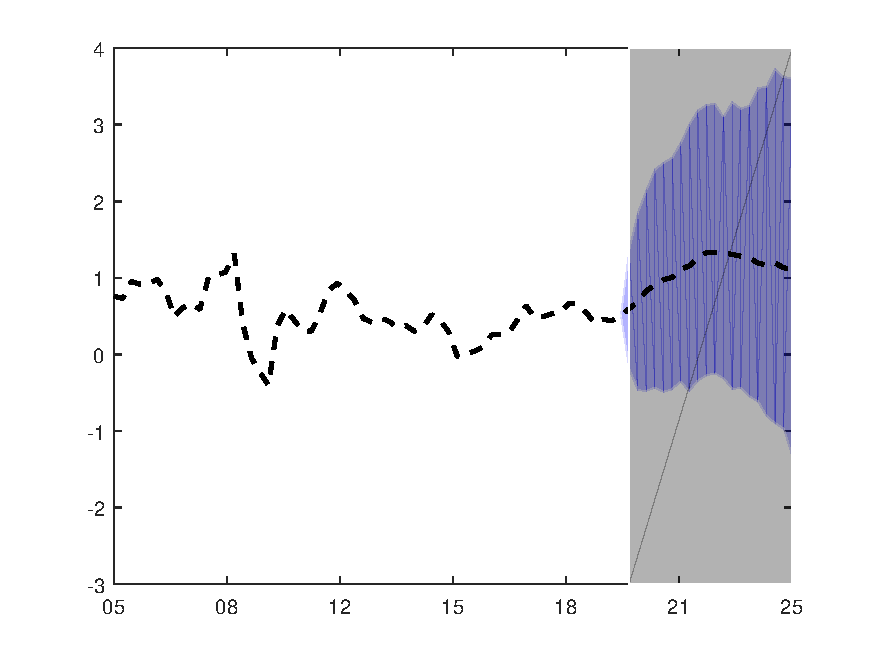
\includegraphics[scale=0.55]{figures/var1_CF3_randomShocks1_normalReg_pi}}}
}

\centerline{
\subfloat[Nominal Rate]{{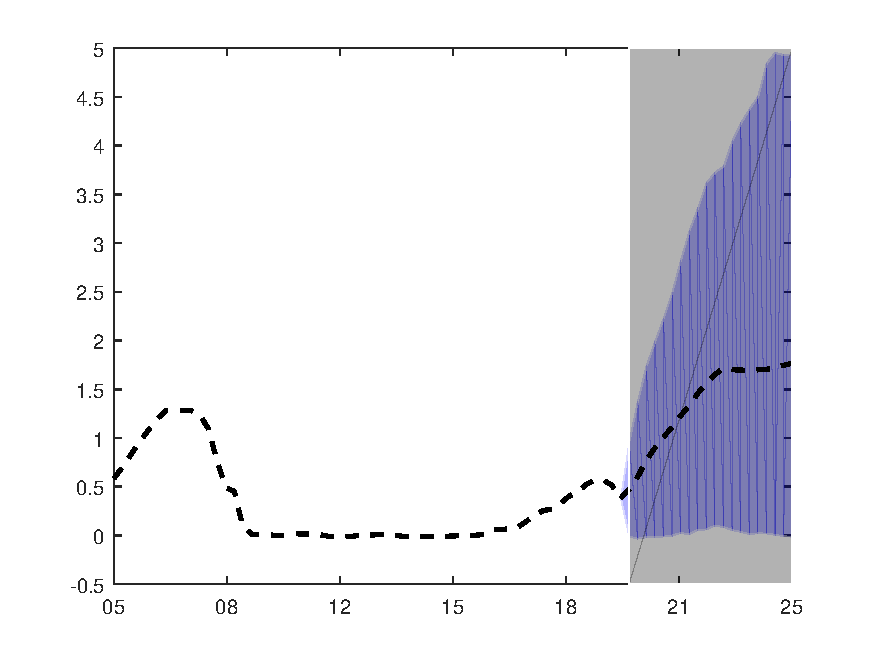
\includegraphics[scale=0.55]{figures/var1_CF3_randomShocks1_normalReg_intRate}}}
\subfloat[Shadow Rate]{{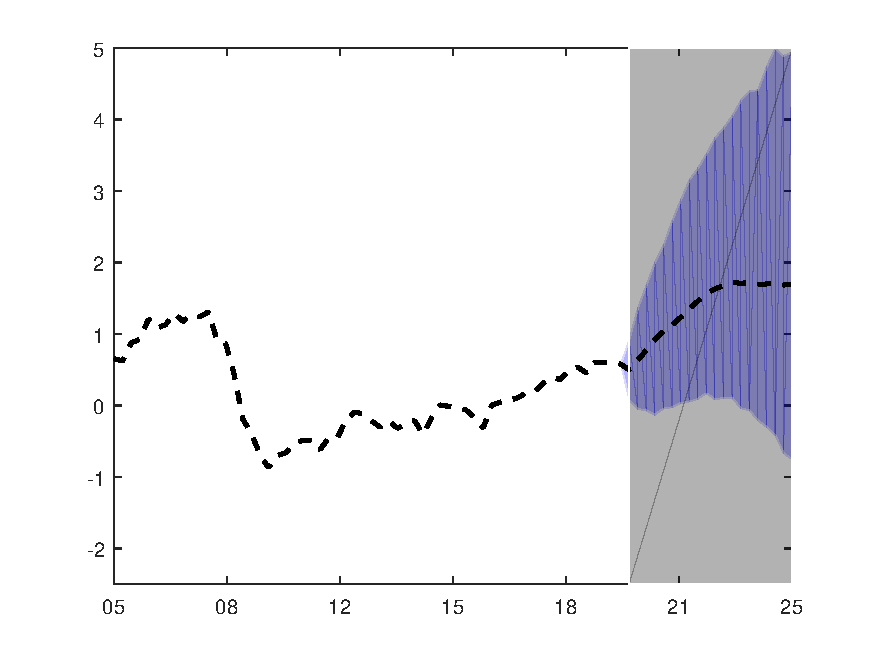
\includegraphics[scale=0.55]{figures/var1_CF3_randomShocks1_normalReg_SR}}}
}

\centerline{
\subfloat[Fraction of de-anchored expectations]{{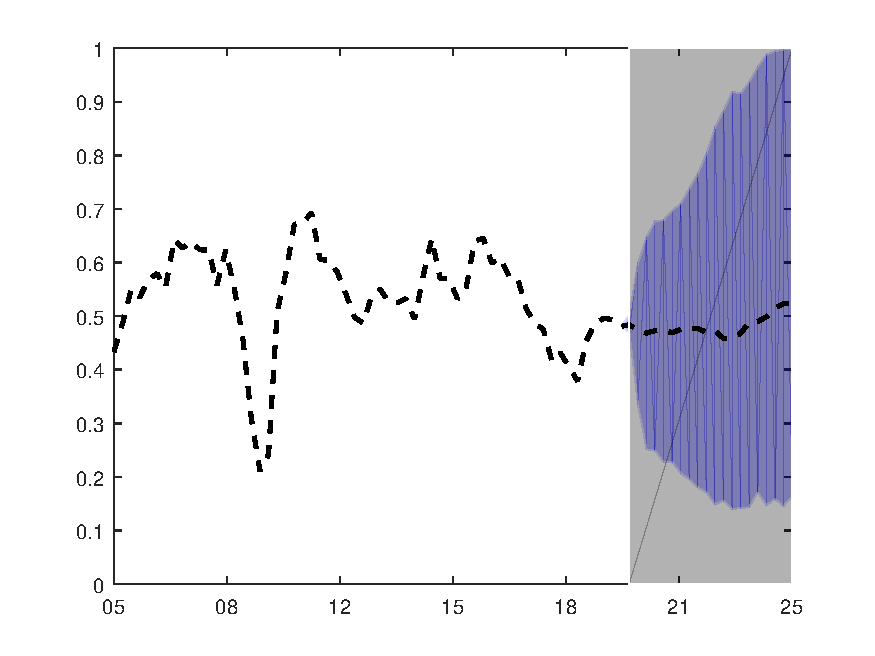
\includegraphics[scale=0.55]{figures/var1_CF3_randomShocks1_normalReg_n1}}}
\subfloat[Taylor Rule Probability]{{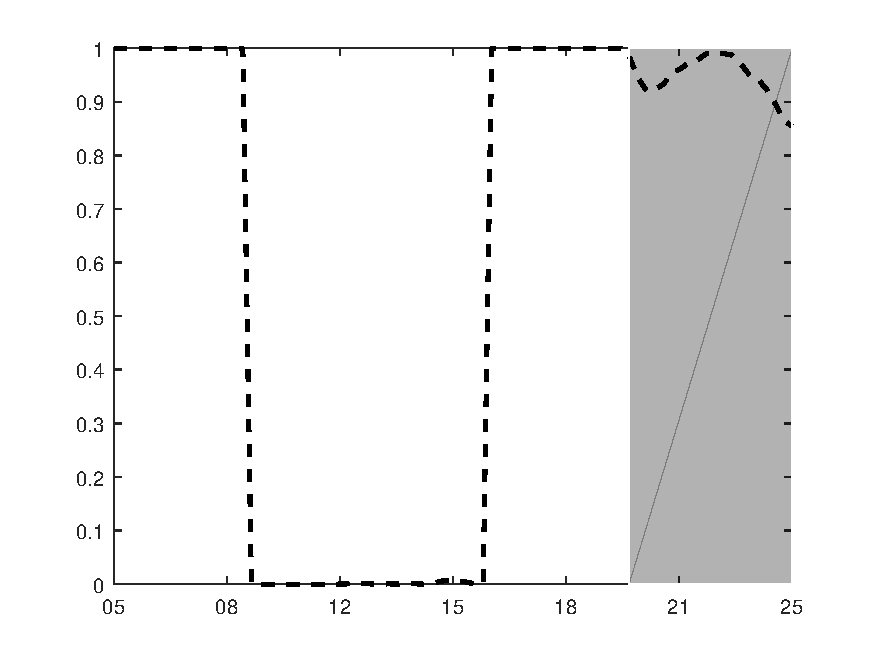
\includegraphics[scale=0.55]{figures/var1_CF3_randomShocks1_normalReg_regimeProb}}}
}

\caption{Counterfactuals with randomized shocks after 2019Q4. Simulations where the average probability of Taylor rule remains above 50\%. }
\end{figure}


\begin{figure}[hbt!]
\centerline{
\subfloat[Output Gap]{{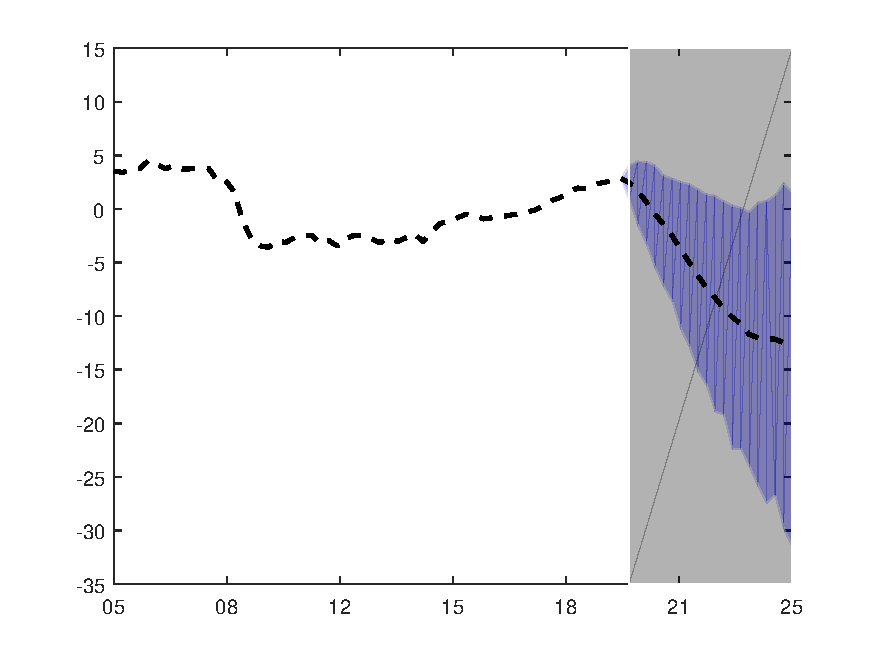
\includegraphics[scale=0.55]{figures/var1_CF3_randomShocks1_zlbReg_gap}}}
\subfloat[Inflation]{{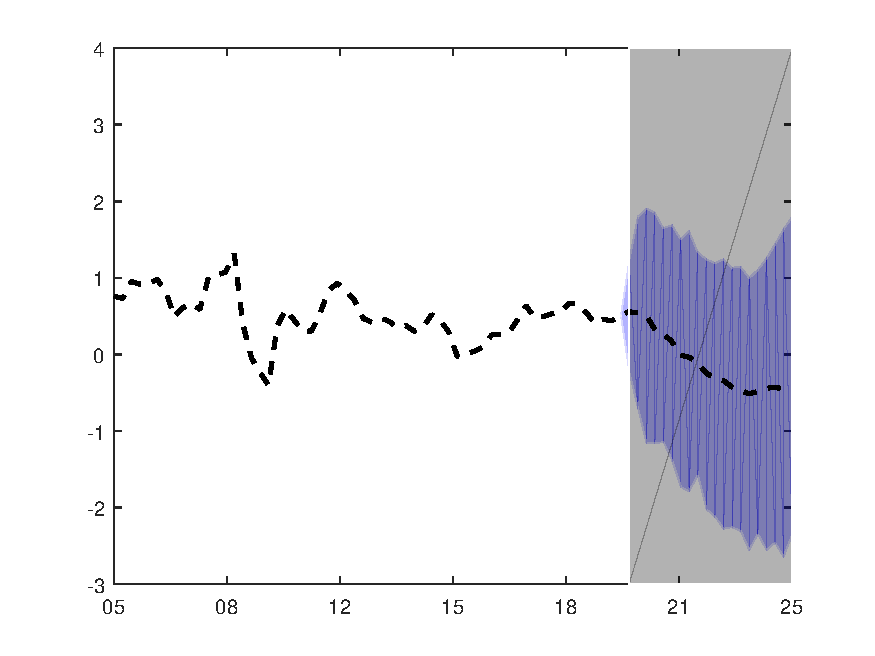
\includegraphics[scale=0.55]{figures/var1_CF3_randomShocks1_zlbReg_pi}}}
}

\centerline{
\subfloat[Nominal Rate]{{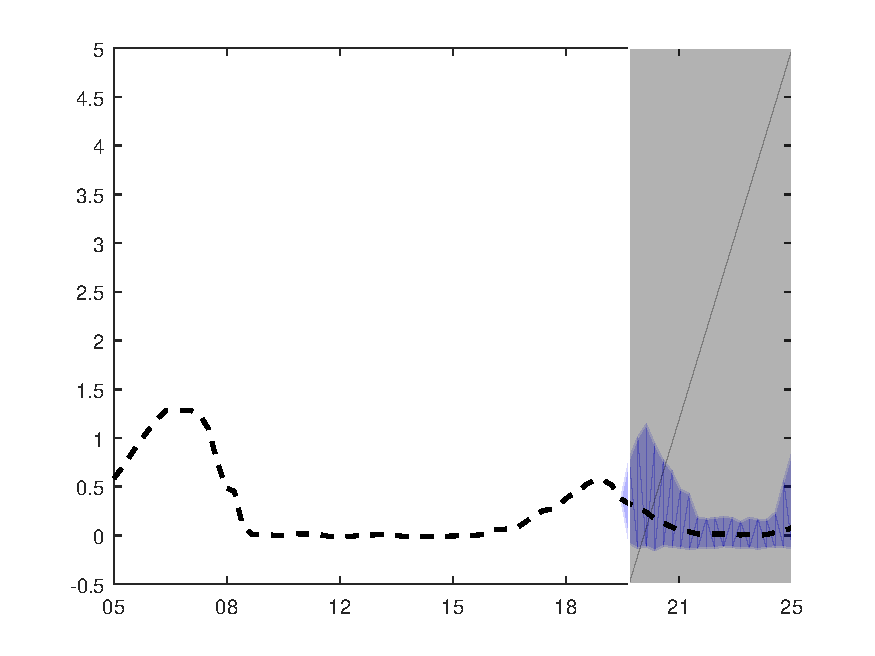
\includegraphics[scale=0.55]{figures/var1_CF3_randomShocks1_zlbReg_intRate}}}
\subfloat[Shadow Rate]{{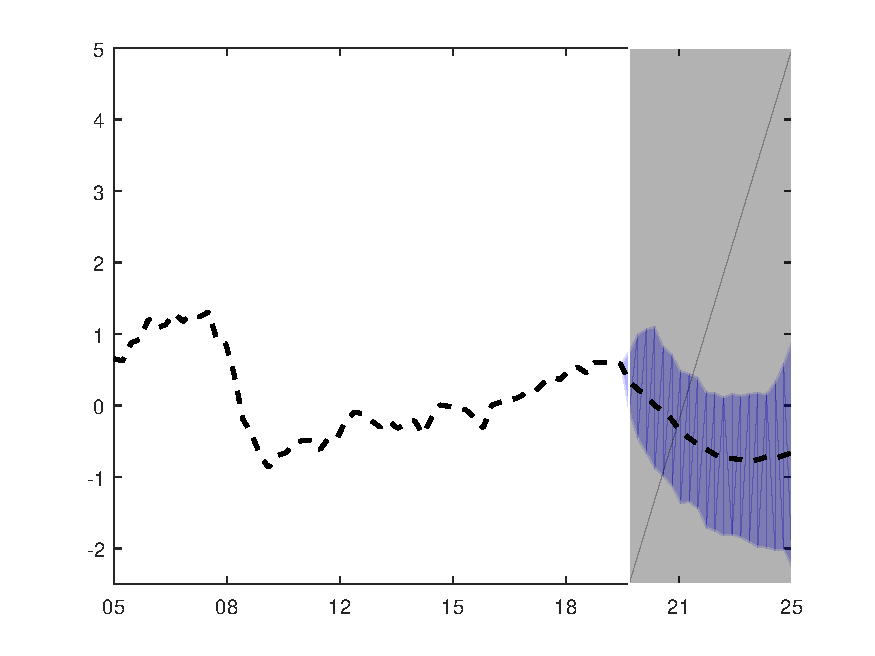
\includegraphics[scale=0.55]{figures/var1_CF3_randomShocks1_zlbReg_SR}}}
}

\centerline{
\subfloat[Fraction of de-anchored expectations]{{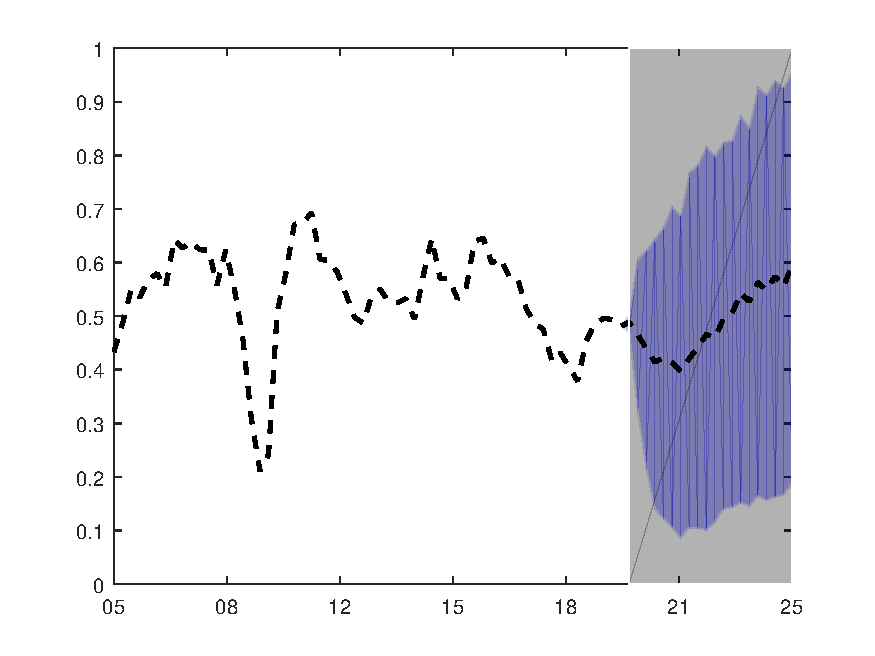
\includegraphics[scale=0.55]{figures/var1_CF3_randomShocks1_zlbReg_n1}}}
\subfloat[Taylor Rule Probability]{{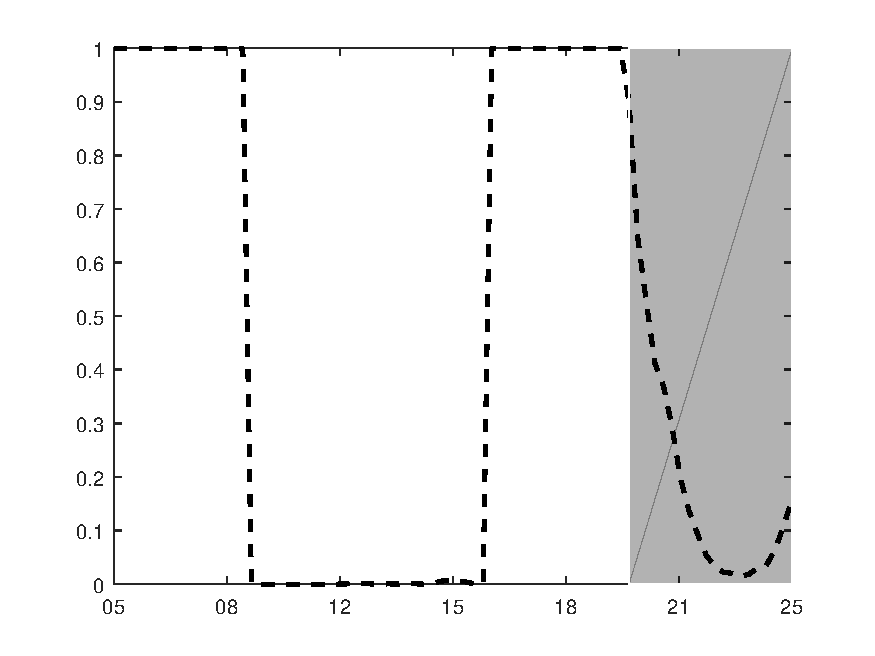
\includegraphics[scale=0.55]{figures/var1_CF3_randomShocks1_zlbReg_regimeProb}}}
}

\caption{Counterfactuals with randomized shocks after 2019Q4. Simulations where the average probability of Taylor rule remains below 50\%. }
\end{figure}


\FloatBarrier

\subsection{Counterfactual IV: post 2019Q4 period with large supply and demand shocks.}


\begin{figure}[hbt!]
\centerline{
\subfloat[Demand Shock]{{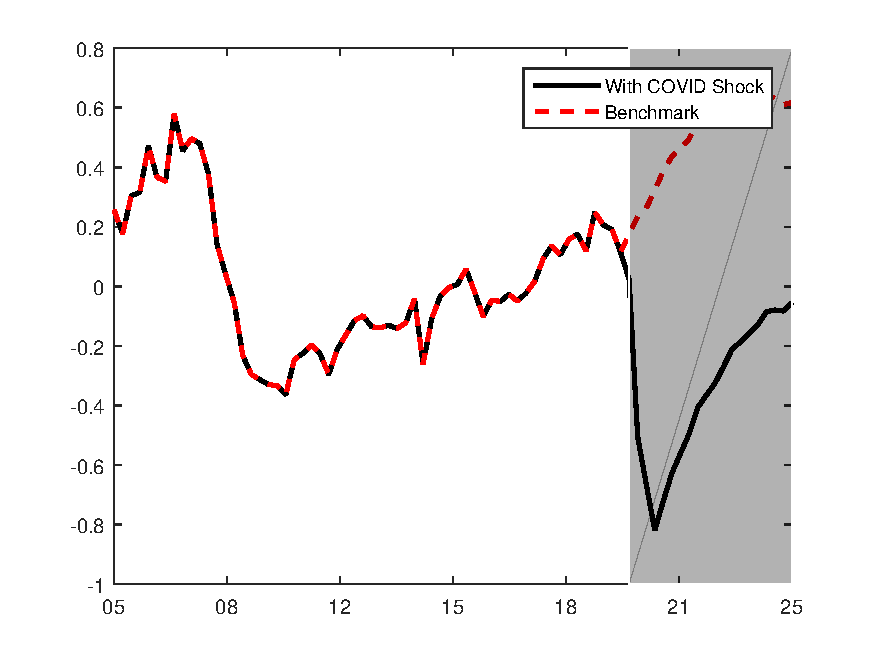
\includegraphics[scale=0.4]{figures/var1_CF4_covidShock_ar1_gap}}}
\subfloat[Supply Shock]{{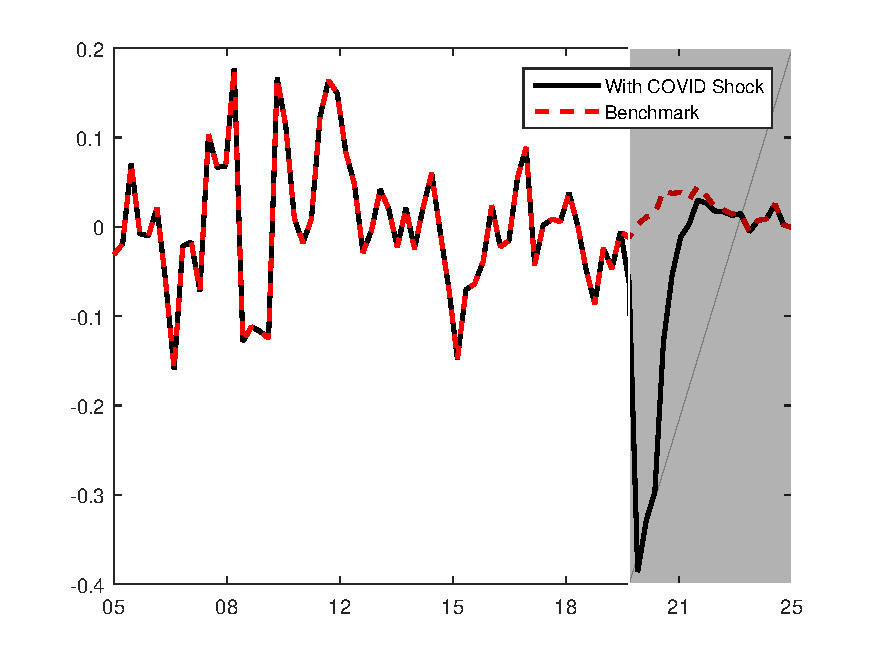
\includegraphics[scale=0.4]{figures/var1_CF4_covidShock_ar1_pi}}}
}

\centerline{
\subfloat[Output Gap]{{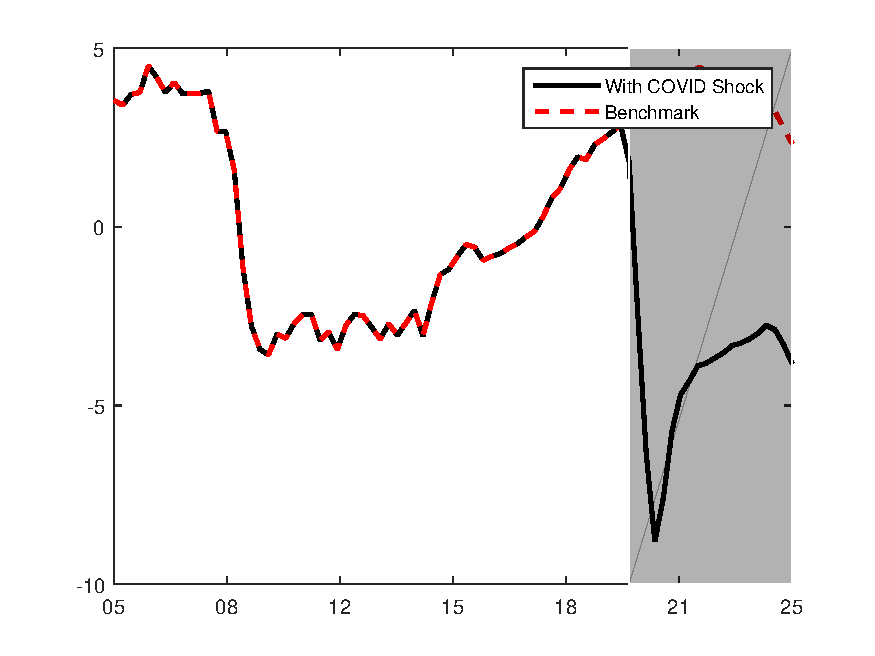
\includegraphics[scale=0.4]{figures/var1_CF4_covidShock_gap}}}
\subfloat[Inflation]{{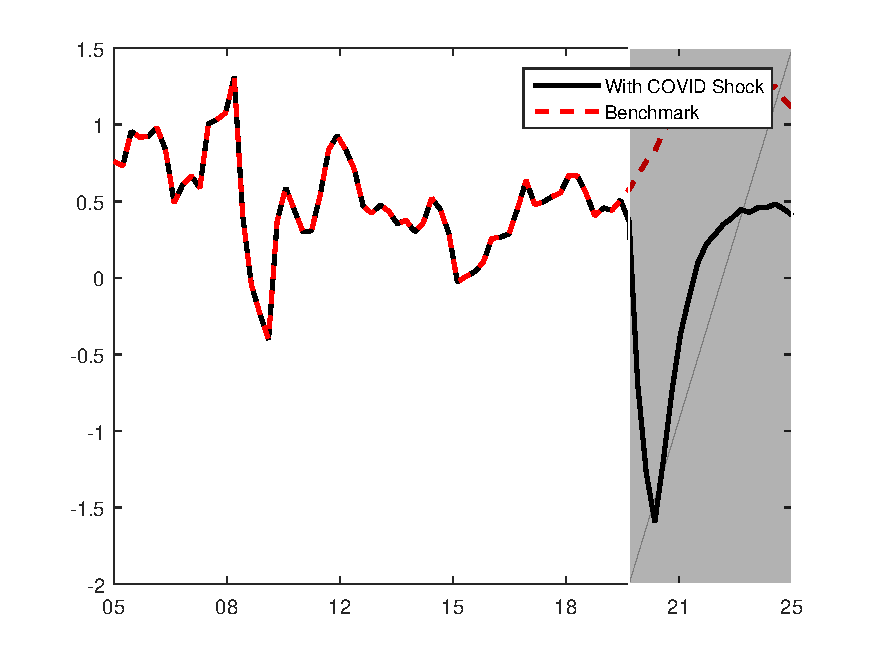
\includegraphics[scale=0.4]{figures/var1_CF4_covidShock_pi}}}
}

\centerline{
\subfloat[Nominal Rate]{{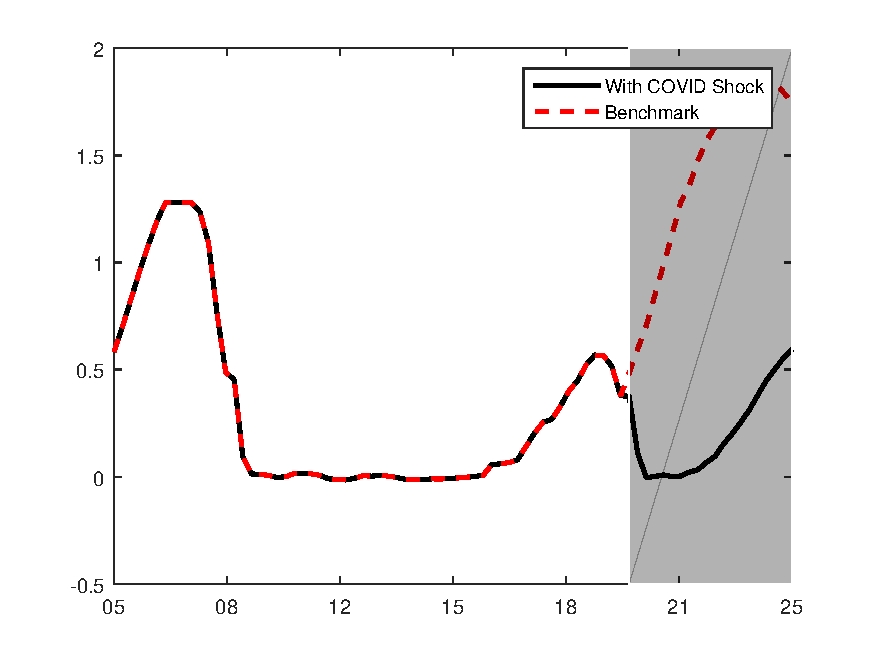
\includegraphics[scale=0.4]{figures/var1_CF4_covidShock_intRate}}}
\subfloat[Shadow Rate]{{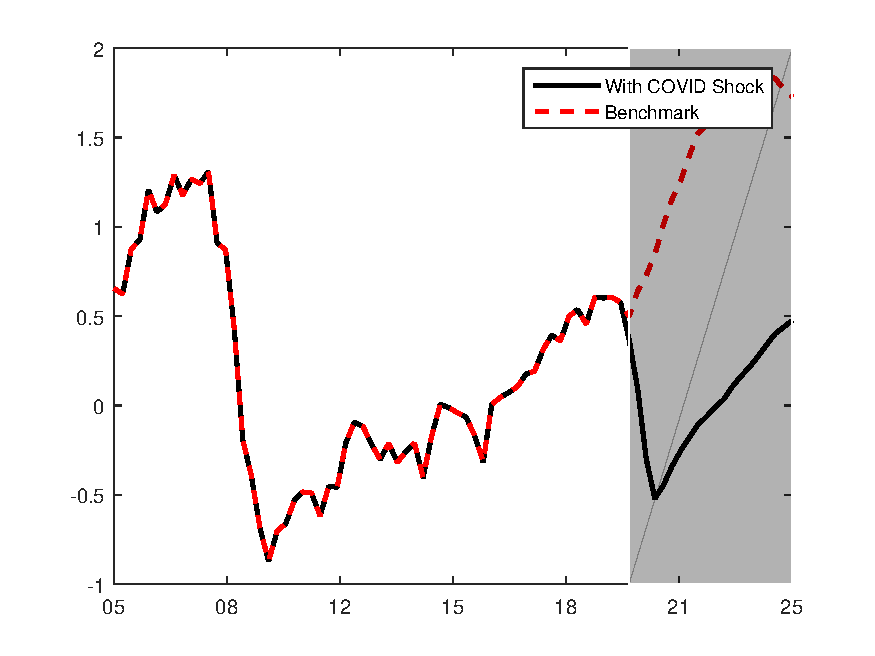
\includegraphics[scale=0.4]{figures/var1_CF4_covidShock_SR}}}
}

\centerline{
\subfloat[Fraction of de-anchored expectations]{{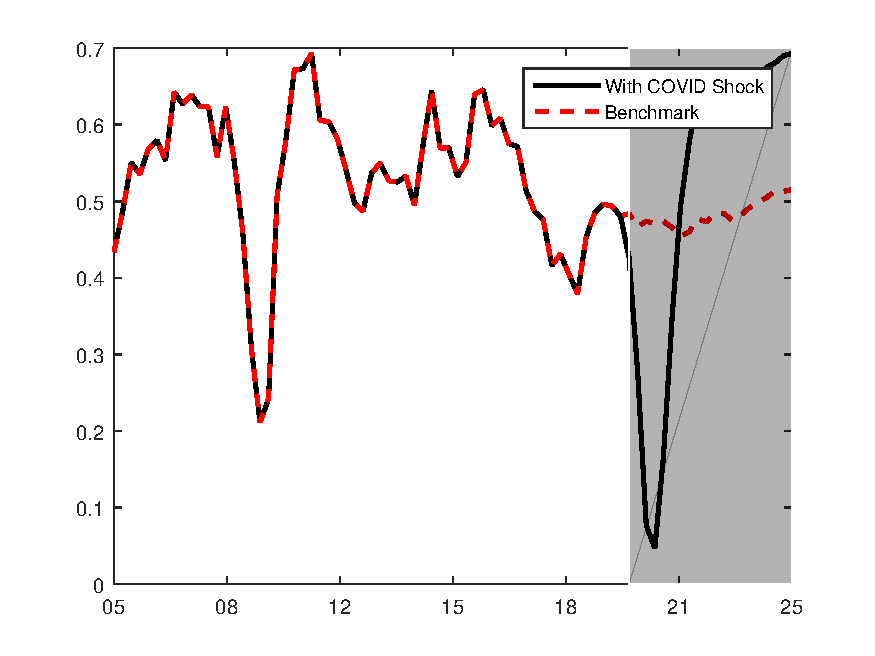
\includegraphics[scale=0.4]{figures/var1_CF4_covidShock_n1}}}
\subfloat[Taylor Rule Probability]{{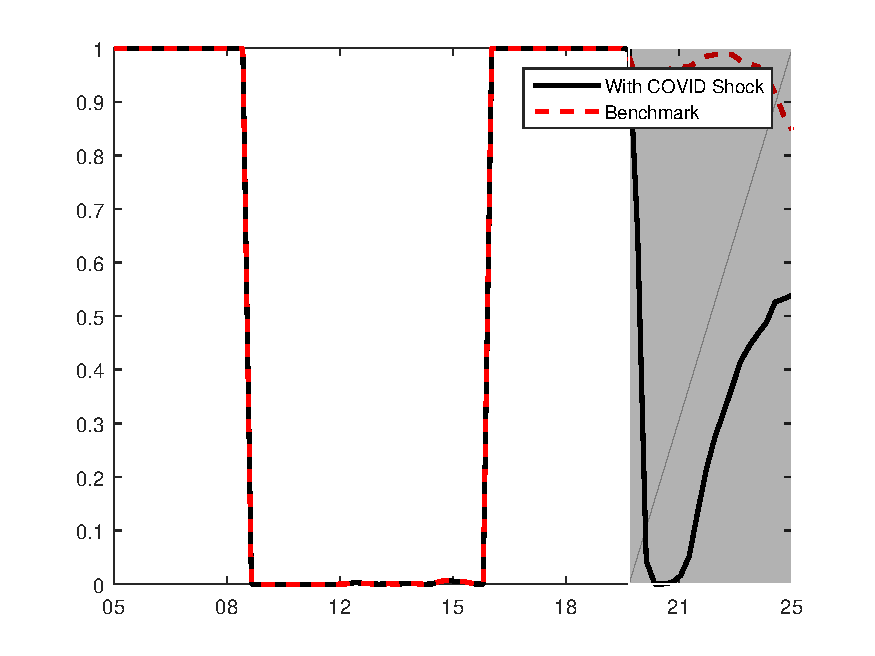
\includegraphics[scale=0.4]{figures/var1_CF4_covidShock_regimeProb}}}
}


\caption{Counterfactuals with randomized shocks after 2019Q4. Simulations where the average probability of Taylor rule remains below 50\%. }
\end{figure}


\FloatBarrier

\subsection{Counterfactual IV: post 2019Q4 period with different fractions of de-anchored expectations.}


\begin{figure}[hbt!]
%\centerline{
%\subfloat[Demand Shock]{{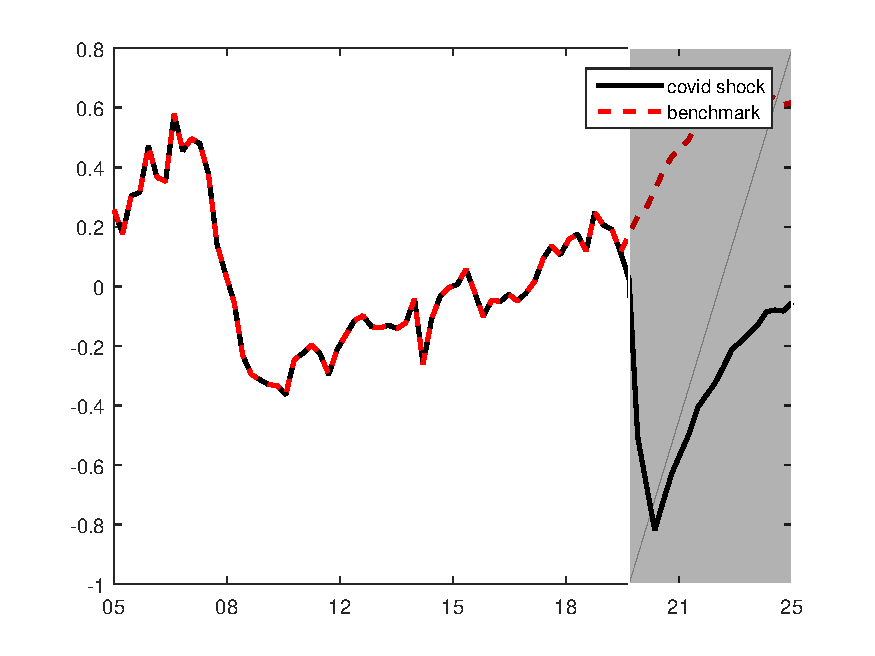
\includegraphics[scale=0.45]{figures/var1_CF5_covidShockFr_ar1_gap}}}
%\subfloat[Supply Shock]{{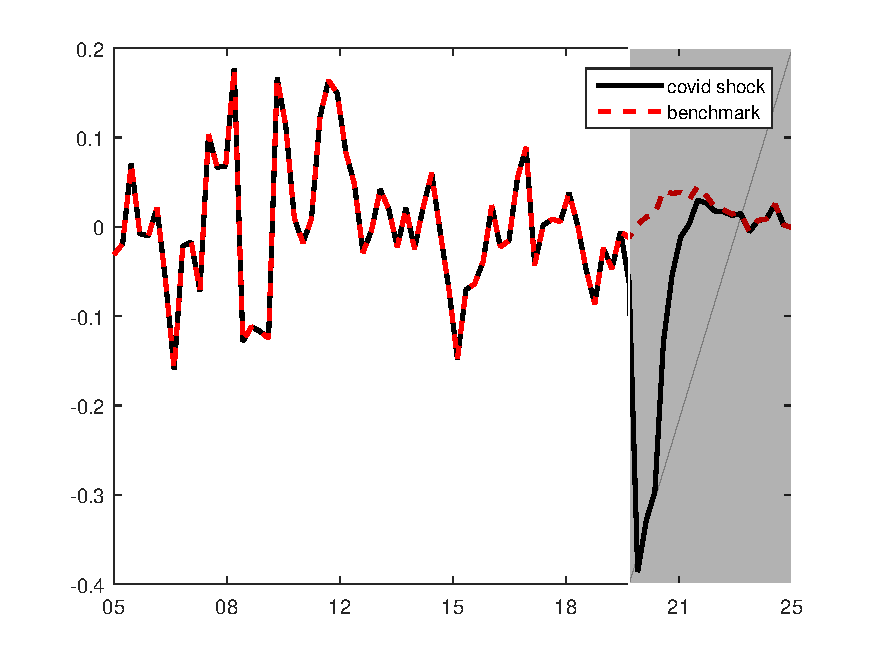
\includegraphics[scale=0.45]{figures/var1_CF5_covidShockFr_ar1_pi}}}
%}

\centerline{
\subfloat[Output Gap]{{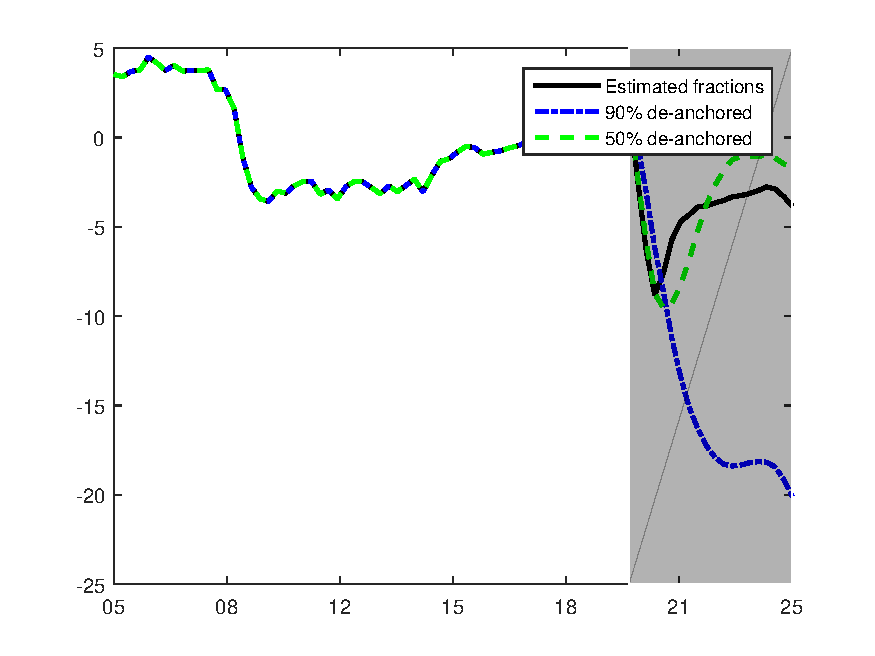
\includegraphics[scale=0.45]{figures/var1_CF5_covidShockFr_gap}}}
\subfloat[Inflation]{{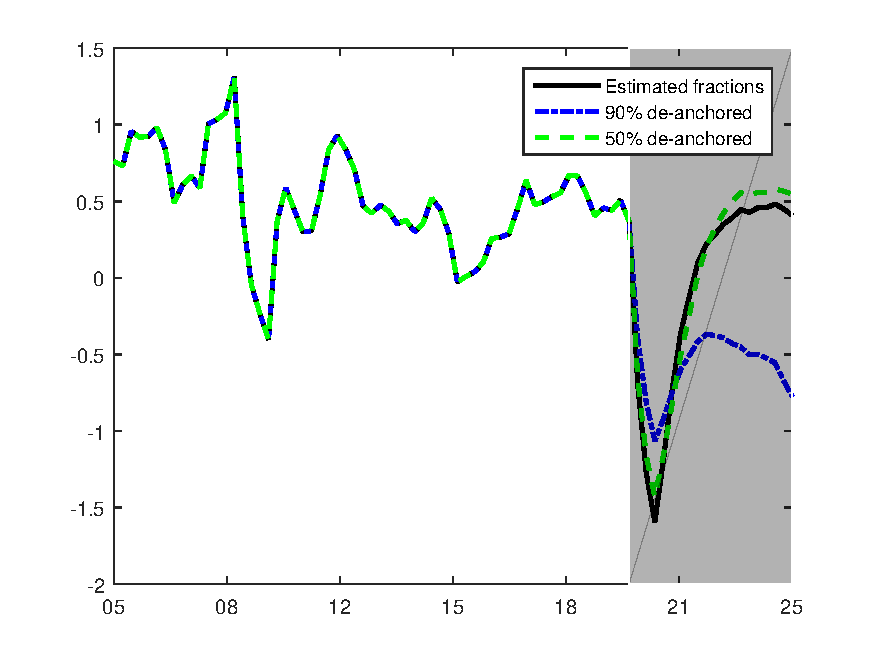
\includegraphics[scale=0.45]{figures/var1_CF5_covidShockFr_pi}}}
}

\centerline{
\subfloat[Nominal Rate]{{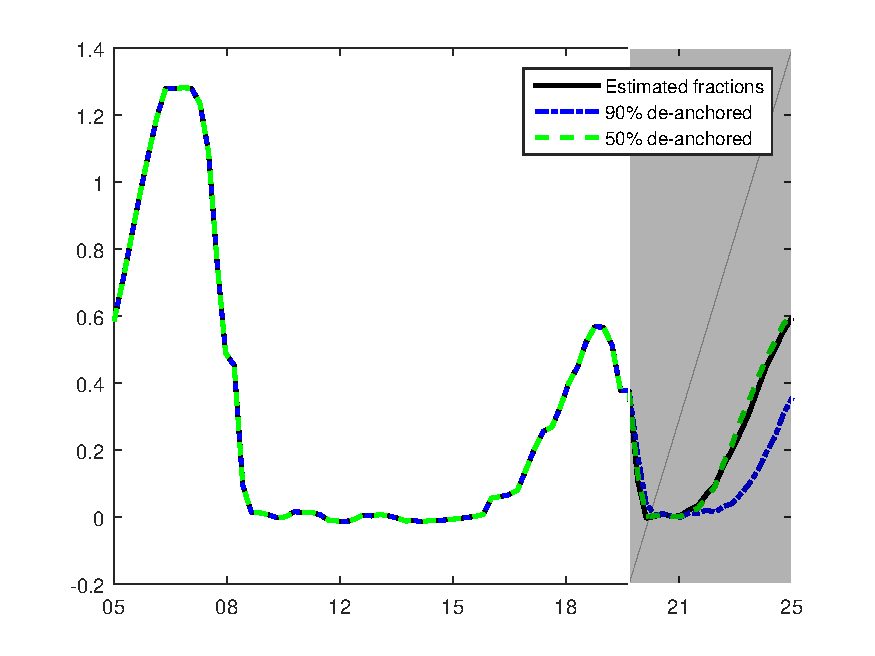
\includegraphics[scale=0.45]{figures/var1_CF5_covidShockFr_intRate}}}
\subfloat[Shadow Rate]{{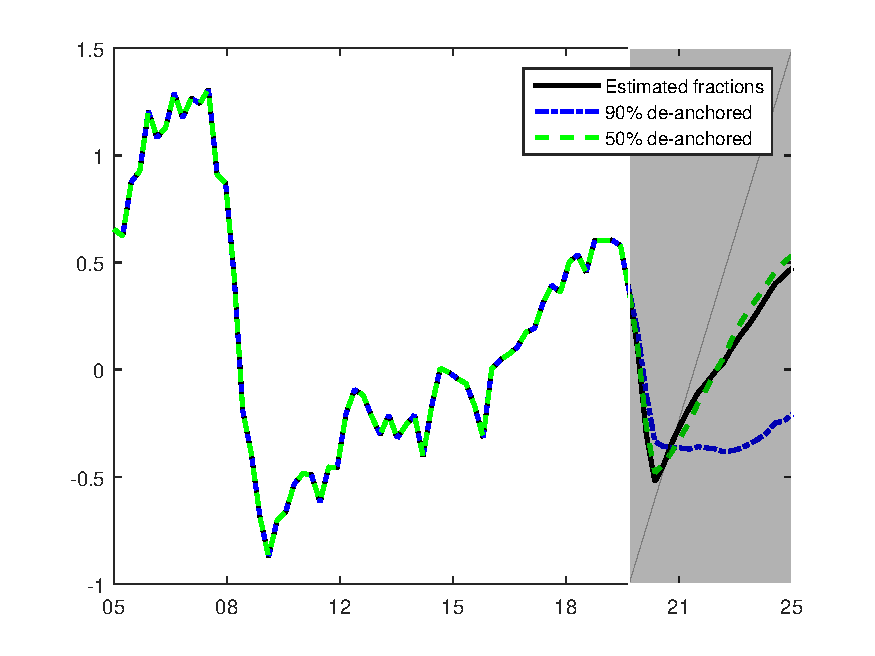
\includegraphics[scale=0.45]{figures/var1_CF5_covidShockFr_SR}}}
}

\centerline{
\subfloat[Fraction of de-anchored expectations]{{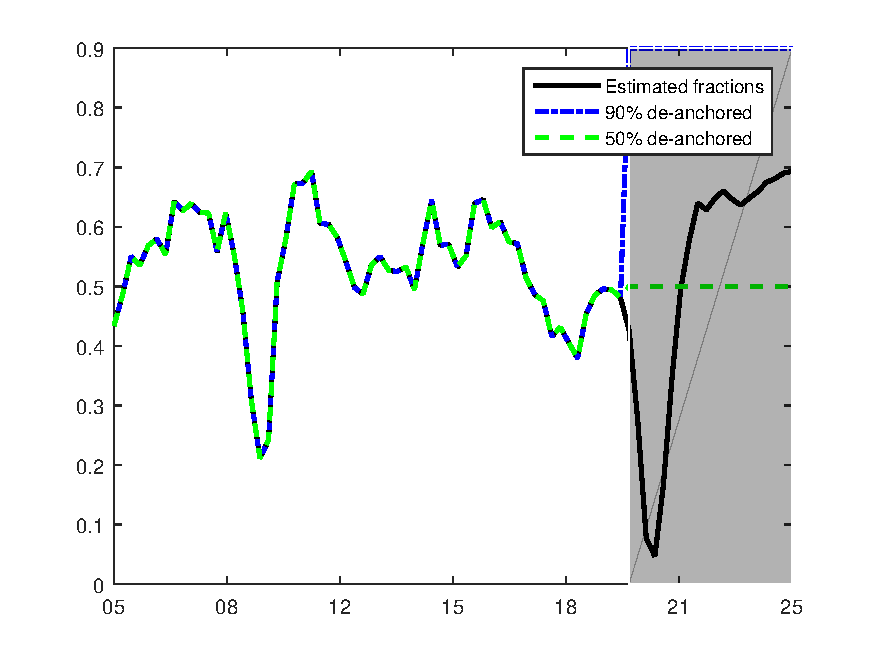
\includegraphics[scale=0.45]{figures/var1_CF5_covidShockFr_n1}}}
\subfloat[Taylor Rule Probability]{{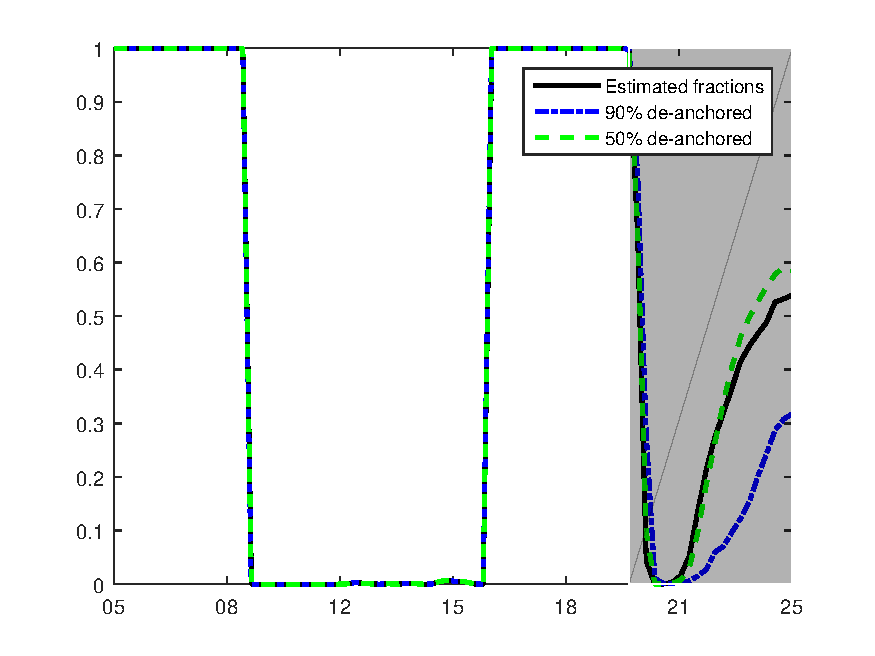
\includegraphics[scale=0.45]{figures/var1_CF5_covidShockFr_regimeProb}}}
}


\caption{Counterfactuals with randomized shocks after 2019Q4. Simulations where the average probability of Taylor rule remains below 50\%. }
\end{figure}


\begin{table}[hbt!]
\begin{tabular}{l|lll|lll}
& VAR(1) & & & AR(1) & & \\
& De-anchoring & & & De-anchoring & & \\
\hline
\hline
Date & Endogenous & 10 \% & 90 \% & Endogenous & 10 \% & 90 \% \\
20Q1 & 99.7\% & 99.7\% & 99.7\% & 99.8\% &99.8\% & 99.8\% \\
20Q2 & 65.2\% & 66.5\% & 76.5\% & 74.4\% &75.1\% &82.2\% \\
20Q3 & 4.3\% & 9.6\% & 27.8\% & 19.8\% & 24.1\% & 39.2\% \\
20Q4 & 0\%  & 0\% &  1\% & 0\% &0\% &7.8\% \\
\hline
\hline
21Q4 & 5.2\% & 2.9\% & 0.5\% & 1.6\% &0.8\% &0.4\% \\
\hline
22Q4 & 31.9\% & 34\% & 7.1\% & 26.1\% &22.4\%& 4.3\% \\
\hline
23Q4 & 46.7\% & 52.6\% & 20.1\% & 45.6\% &43.3\% &14.9\%\\
\hline
24Q4 & 53.9\% & 58.5\% & 31.7\% & 59.4\% &61.1\% &36.5\%\\
\hline
\hline

\end{tabular}
\end{table}


\FloatBarrier

\section{Conclusion}

\FloatBarrier

\section*{Appendix}

\begin{appendix}

\section{Data Descriptions}

-time series names, sources and periods

\section{Posterior Distributions, Diagnostic Checks and Alternative Estimations}

\begin{figure}[hbt!]
\subfloat[REE]{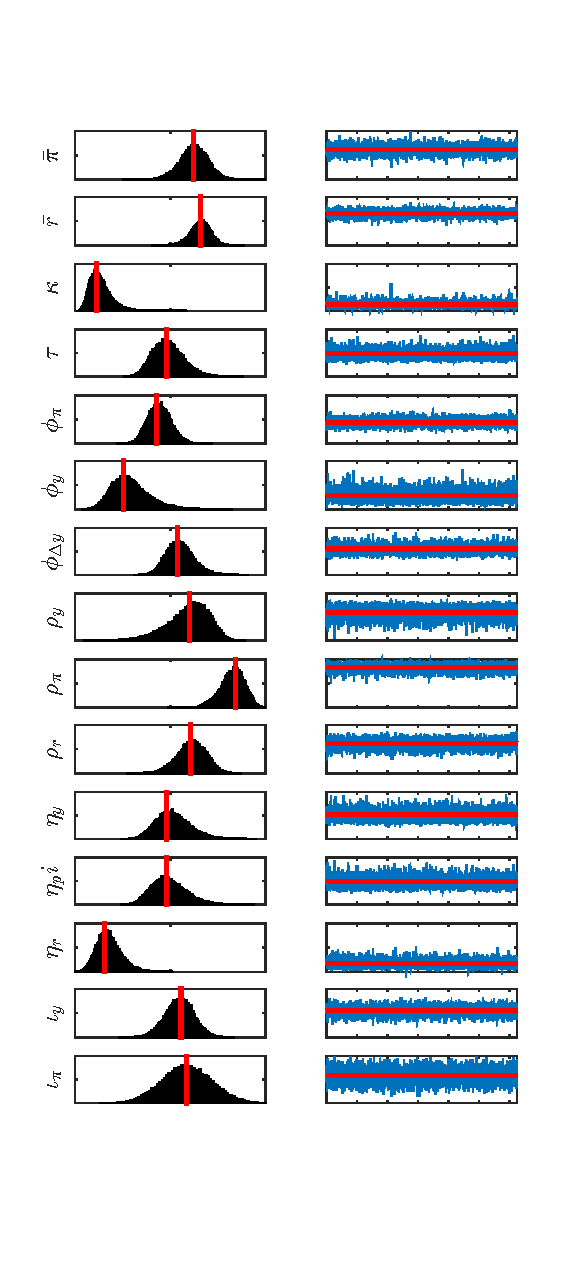
\includegraphics[]{figures/posteriorDist_ree.pdf}}
\subfloat[RISE]{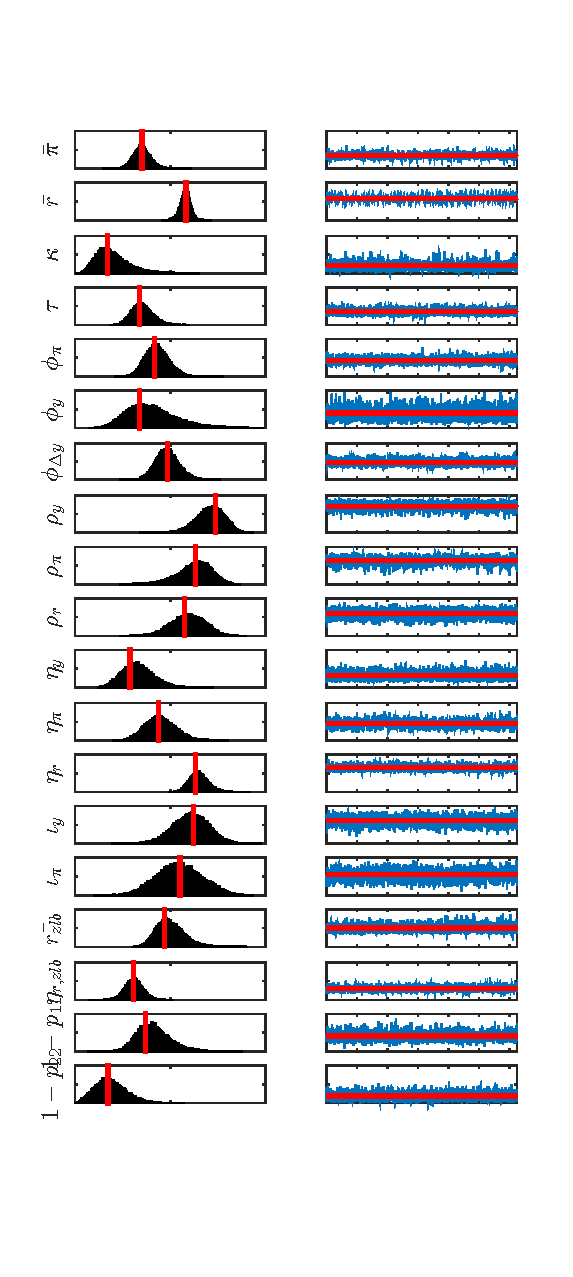
\includegraphics[]{figures/posteriorDist_rise.pdf}}
\caption{Rational Expectations models.}
\end{figure}

\begin{figure}[hbt!]
\subfloat[2-regime]{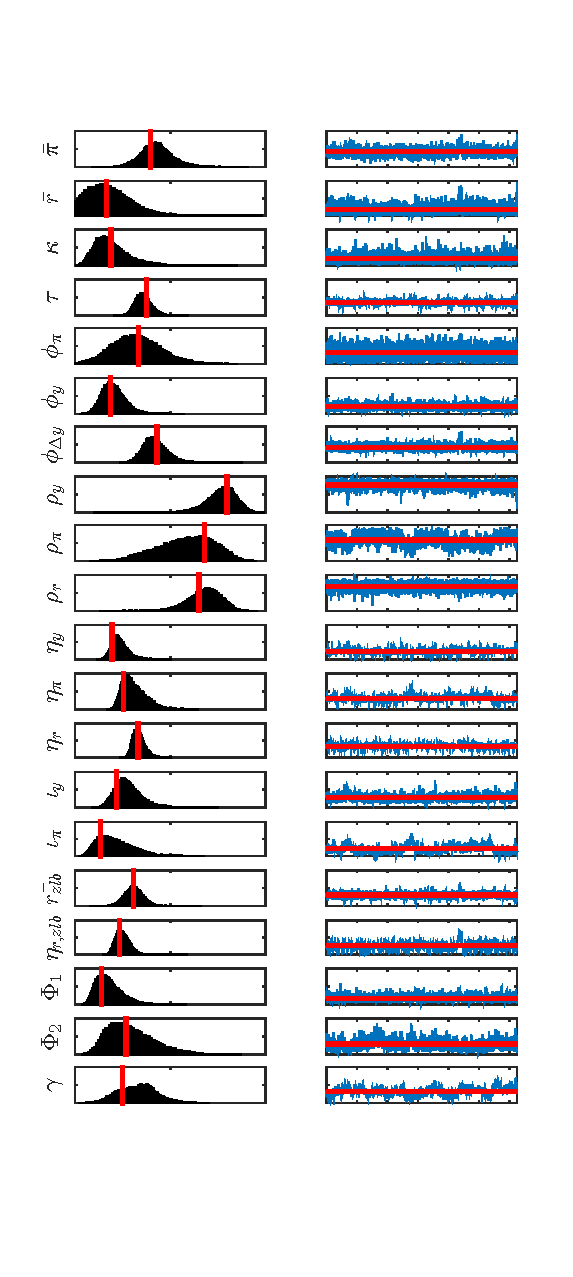
\includegraphics[]{figures/posteriorDist_var1_2regime.pdf}}
\subfloat[4-regime]{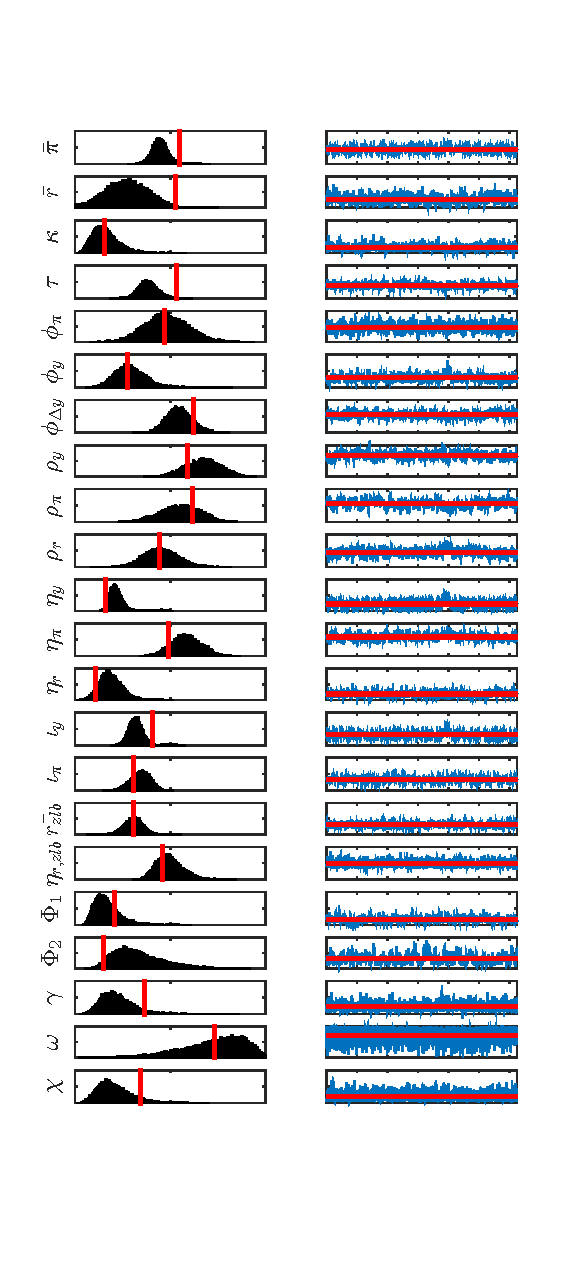
\includegraphics[]{figures/posteriorDist_var1_4regime.pdf}}
\caption{VAR(1) learning models.}
\end{figure}

\begin{figure}[hbt!]
\subfloat[2-regime]{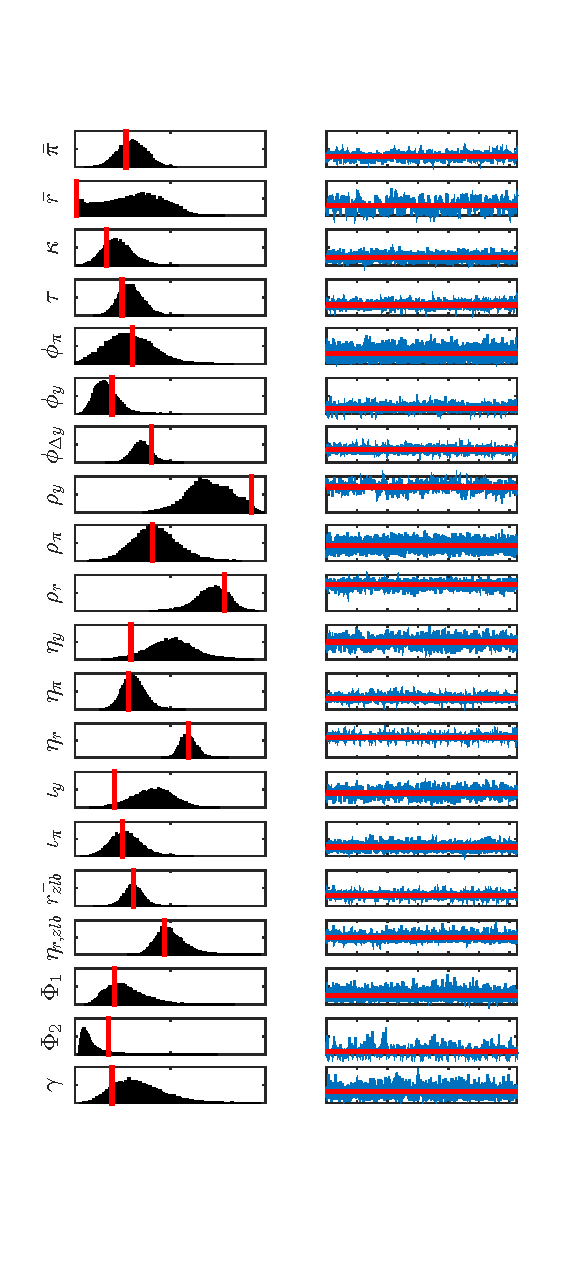
\includegraphics[]{figures/posteriorDist_ar1_2regime.pdf}}
\subfloat[4-regime]{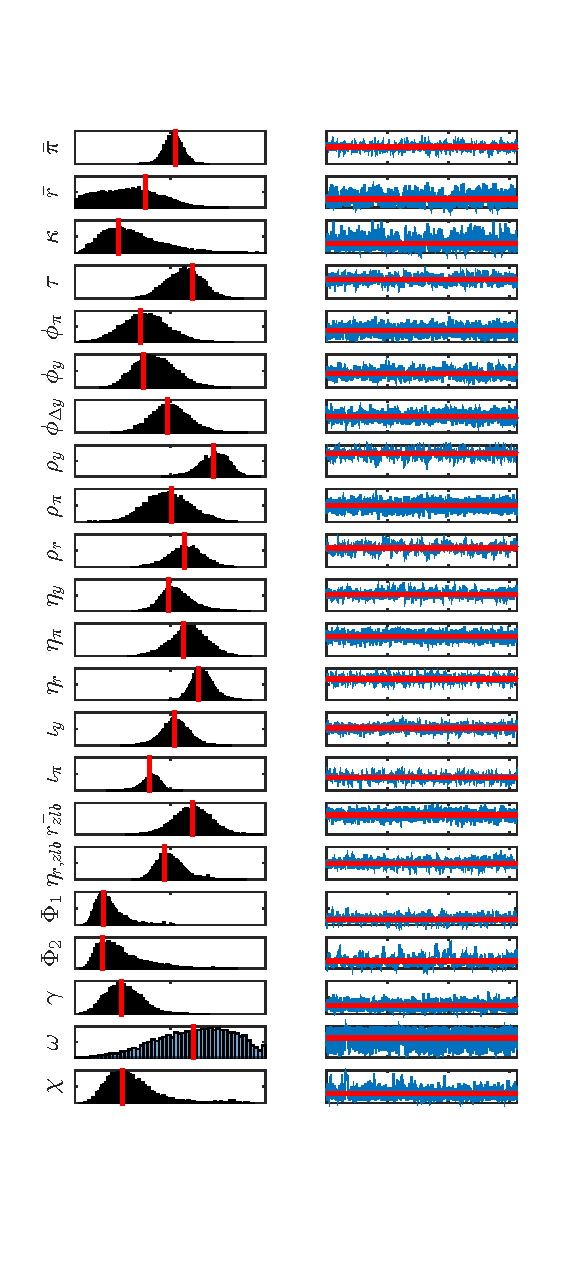
\includegraphics[]{figures/posteriorDist_ar1_4regime.pdf}}
\caption{AR(1) learning models.}
\end{figure}



\begin{table}[hbt!]
\begin{tabular}{l||llllll}
 & Test Result &  &  &  &  &  \\
Tapering Step & REE & RISE & VAR(1) & VAR(1) & AR(1)& AR(1)\\
  & 1-regime & 2-regime & 2-regime & 4-regime & 2-regime &4-regime \\
\hline
\hline
4\% & 39\% & 79\% & 18\% & 52\% & 88\% & 50\% \\
8\% & 35\% & 75\% & 23\% & 57\% & 89\% & 50\% \\
15\% & 32\% & 71\% & 26\% & 56\% & 89\% & 47\%
\end{tabular}
\caption{Geweke's Convergence Diagnostics (1992, 1999). The table reports the p-values of the tests with different tapering steps (4\%, 8\% and 15\% respectively). The test compares the means of the first 20\% and last 50\% of the posterior draws after discarding the burn-in sample. The p-values are all well above 5\% indicating a failure to reject the null hypothesis that the distributions are different at the beginning and end of the sample. }
\end{table}




estimation results with cbo's measure of output gap also goes here

\FloatBarrier

\section{Estimated Time Series of Other Learning Variables }

-VAR(1)-4 regime goes into main text, report the remaining 3 models here

\FloatBarrier

\section{Estimation Method Description}

provide a short summary of the Kim-Nelson setup, refer to the previous paper. 

\FloatBarrier

%\section{Monte Carlo Simulations}

%simulations of the 4-regime learning models to understand the ergodic distributions of such models. This is a BIG MAYBE, to be considered after the other sections are finished. 

\end{appendix}


\end{document}